%%%% Time-stamp: <2017-02-05 16:13:04 vk>
%% ========================================================================
%%%% Disclaimer
%% ========================================================================
%%
%% created by
%%
%%      Karl Voit
%%

%% ========================================================================
%%%% Basic settings
%% ========================================================================
%% (idea of using newcommands for basic documentclass settings from: Thomas Schlager)

\newcommand{\mypapersize}{A4}
%% e.g., "A4", "letter", "legal", "executive", ...
%% The size of the paper of the resulting PDF file.

\newcommand{\mylaterality}{twoside}
%% "oneside" or "twoside"
%% Either you are creating a document which is printed on both, left pages
%% and right pages (twoside) or you create a document which is printed
%% on right pages only (oneside).

\newcommand{\mydraft}{false}
%% "true" or "false"
%% Use draft mode? If true, included graphics are replaced by empty
%% rectangles (of same size) and overfull boxes (in margin space) are
%% marked with black box (-> easy to spot!)

\newcommand{\myparskip}{half}
%% e.g., "no", "full", "half", ...
%% How to separate paragraphs: indention ("no") or spacing ("half",
%% "full", ...).

\newcommand{\myBCOR}{0mm}
%% Inner binding correction. This value depends on the method which is
%% being used to bind your printed result. Some techniques do not
%% require a binding correction at all ("0mm"), other require for
%% example "5mm". Refer to KOMA script documentation for a detailed
%% explanation what a binding correction is and how to measure it.

\newcommand{\myfontsize}{12pt}
%% e.g., 10pt, 11pt, 12pt
%% The font size of the main text in pt (points).

\newcommand{\mylinespread}{1.0}
%% e.g., 1.0, 1.5, 2.0
%% Line spacing in %/100. For example 1.5 means 150% of the usual line
%% spacing. Please use with caution: 100% ("1.0") is fine because the
%% font was designed for it.

\newcommand{\mylanguage}{ngerman,american}
%% "english,ngerman", "ngerman,english", ...
%% NOTE: The *last* language is the active one!
%% See babel documentation for further details.

%% BibLaTeX-settings: (see biblatex reference for further description)
\newcommand{\mybiblatexstyle}{authoryear}
%% e.g., "alphabetic", "authoryear", ...
%% The biblatex style which is being used for referencing. See
%% biblatex documentation for further details and more values.
%%
%% CAUTION: if you change the style, please check for (in)compatible
%%          "biblatex" package options in the file
%%          "template/preamble.tex"! For example: "alphabetic" does
%%          not have an option "dashed=..." and causes an error if it
%%          does not get removed from the list of options.

\newcommand{\mybiblatexdashed}{false}  %% "true" or "false"
%% If true: replace recurring reference authors with a dash.

\newcommand{\mybiblatexbackref}{true}  %% "true" or "false"
%% If true: create backward links from reference to citations.

\newcommand{\mybiblatexfile}{references-biblatex.bib}
%% Name of the biblatex file that holds the references.

\newcommand{\mydispositioncolor}{30,103,182}
%% e.g., "30,103,182" (blue/turquois), "0,0,0" (black), ...
%% Color of the headings and so forth in RGB (red,green,blue) values.
%% NOTE: if you are using "0,0,0" for black, printers might still
%%       recognize pages as color pages. In case this is a problem
%%       (paying for color print-outs vs. paying for b/w-printouts)
%%       please edit file "template/preamble.tex" and change
%%       "\definecolor{DispositionColor}{RGB}{\mydispositioncolor}"
%%       to "\definecolor{DispositionColor}{gray}{0}" and thus
%%       overwriting the value of \mydispositioncolor above.

\newcommand{\mycolorlinks}{true}  %% "true" or "false"
%% Enables or disables colored links (hyperref package).

\newcommand{\mytitlepage}{template/title_Thesis_TU_Graz}
%% Your own or one of following pre-defined title pages:
%% "template/title_plain_maketitle": simple maketitle page
%% "template/title_Diplomarbeit_KF_Uni_Graz.tex": fancy (german) title page for KF Uni Graz
%% "template/title_Thesis_TU_Graz":
%%             titlepage for Graz University of Technology (correct
%%             (old?) Corporate Design) by Karl Voit (2012)
%% "template/title_Thesis_TU_Graz_-_kazemakase":
%%             titlepage for Graz University of Technology
%%             (correct new Corporate Design) by kazemakase (2013):
%%             see https://github.com/novoid/LaTeX-KOMA-template/issues/5
%% "template/title_VWA": titlepage for Vorwissenschaftliche Arbeit

\newcommand{\mytodonotesoptions}{}
%% e.g., "" (empty), "disable", ...
%% Options for the todonotes-package. If "disable", all todonotes will
%% be hidden (including listoftodos).

%% Load main settings for document preamble:
%% Time-stamp: <2015-04-30 17:23:24 vk>
%%%% === Disclaimer: =======================================================
%% created by
%%
%%      Karl Voit
%%
%% using GNU/Linux, GNU Emacs & LaTeX 2e
%%

%doc% %% overriding preamble/preamble.tex %%
%doc% \newcommand{\mylinespread}{1.0}  \newcommand{\mycolorlinks}{true}
%doc% \documentclass[12pt,paper=a4,parskip=half,DIV=calc,oneside,%%
%doc% headinclude,footinclude=false,open=right,bibliography=totoc]{scrartcl}
%doc% \usepackage[utf8]{inputenc}\usepackage[ngerman,american]{babel}\usepackage{scrpage2}
%doc% \usepackage{ifthen}\usepackage{eurosym}\usepackage{xspace}\usepackage[usenames,dvipsnames]{xcolor}
%doc% \usepackage[protrusion=true,factor=900]{microtype}
%doc% \usepackage{enumitem}
%doc% \usepackage[pdftex]{graphicx}
%doc% \usepackage{todonotes}
%doc% \usepackage{dingbat,bbding} %% special characters
%doc% \definecolor{DispositionColor}{RGB}{30,103,182}
%doc%
%doc% \usepackage[backend=biber,style=authoryear,dashed=false,natbib=true,hyperref=true%%
%doc% ]{biblatex}
%doc%
%doc% \addbibresource{references-biblatex.bib} %% remove, if using BibTeX instead of biblatex
%doc%
%doc% %% overriding userdata %%
%doc% \newcommand{\myauthor}{Karl Voit}\newcommand{\mytitle}{LaTeX Template Documentation}
%doc% \newcommand{\mysubject}{A Comprehensive Guide to Use the
%doc% Template from https://github.com/novoid/LaTeX-KOMA-template}
%doc% \newcommand{\mykeywords}{LaTeX, pdflatex, template, documentation, biber, biblatex}
%doc%
%doc% \newcommand{\myLaT}{\LaTeX{}@TUG\xspace}
%doc%
%doc% %% for future use?
%doc% % \usepackage{filecontents}
%doc% % \begin{filecontents}{filename.example}
%doc% %
%doc% % \end{filecontents}
%doc%
%doc%
%doc% %% using existing TeX files %%
%doc% %% Time-stamp: <2015-04-30 17:19:58 vk>
%%%% === Disclaimer: =======================================================
%% created by
%%
%%      Karl Voit
%%
%% using GNU/Linux, GNU Emacs & LaTeX 2e
%%

%doc%
%doc% \section{\texttt{mycommands.tex} --- various definitions}\myinteresting
%doc% \label{sec:mycommands}
%doc%
%doc% In file \verb#template/mycommands.tex# many useful commands are being
%doc% defined. 
%doc% 
%doc% \paragraph{What should I do with this file?} Please take a look at its 
%doc% content to get the most out of your document.
%doc% 

%doc% 
%doc% One of the best advantages of \LaTeX{} compared to \myacro{WYSIWYG} software products is
%doc% the possibility to define and use macros within text. This empowers the user to
%doc% a great extend.  Many things can be defined using \verb#\newcommand{}# and
%doc% automates repeating tasks. It is recommended to use macros not only for
%doc% repetitive tasks but also for separating form from content such as \myacro{CSS}
%doc% does for \myacro{XHTML}. Think of including graphics in your document: after
%doc% writing your book, you might want to change all captions to the upper side of
%doc% each figure. In this case you either have to modify all
%doc% \texttt{includegraphics} commands or you were clever enough to define something
%doc% like \verb#\myfig#\footnote{See below for a detailed description}. Using a
%doc% macro for including graphics enables you to modify the position caption on only
%doc% \emph{one} place: at the definition of the macro.
%doc% 
%doc% The following section describes some macros that came with this document template
%doc% from \myLaT and you are welcome to modify or extend them or to create
%doc% your own macros!
%doc% 

%doc% 
%doc% \subsection{\texttt{myfig} --- including graphics made easy}
%doc% 
%doc% The classic: you can easily add graphics to your document with \verb#\myfig#:
%doc% \begin{verbatim}
%doc%  \myfig{flower}%% filename w/o extension in the folder figures
%doc%        {width=0.7\textwidth}%% maximum width/height, aspect ratio will be kept
%doc%        {This flower was photographed at my home town in 2010}%% caption
%doc%        {Home town flower}%% optional (short) caption for list of figures
%doc%        {fig:flower}%% label
%doc% \end{verbatim}
%doc% 
%doc% There are many advantages of this command (compared to manual
%doc% \texttt{figure} environments and \texttt{includegraphics} commands:
%doc% \begin{itemize}
%doc% \item consistent style throughout the whole document
%doc% \item easy to change; for example move caption on top
%doc% \item much less characters to type (faster, error prone)
%doc% \item less visual clutter in the \TeX{}-files
%doc% \end{itemize}
%doc% 
%doc% 
\newcommand{\myfig}[5]{
%% example:
% \myfig{}%% filename in figures folder
%       {width=0.5\textwidth,height=0.5\textheight}%% maximum width/height, aspect ratio will be kept
%       {}%% caption
%       {}%% optional (short) caption for list of figures
%       {}%% label
\begin{figure}%[htp]
  \centering
  \includegraphics[keepaspectratio,#2]{figures/#1}
  \caption[#4]{#3}
  \label{#5} %% NOTE: always label *after* caption!
\end{figure}
}


%doc% 
%doc% \subsection{\texttt{myclone} --- repeat things!}
%doc% 
%doc% Using \verb#\myclone[42]{foobar}# results the text \enquote{foobar} printed 42 times.
%doc% But you can not only repeat text output with \texttt{myclone}. 
%doc%
%doc% Default argument
%doc% for the optional parameter \enquote{number of times} (like \enquote{42} in the example above) 
%doc% is set to two.
%doc% 
%% \myclone[x]{text}
\newcounter{myclonecnt}
\newcommand{\myclone}[2][2]{%
  \setcounter{myclonecnt}{#1}%
  \whiledo{\value{myclonecnt}>0}{#2\addtocounter{myclonecnt}{-1}}%
}

%old% %d oc% 
%old% %d oc% \subsection{\texttt{fixxme} --- sidemark something as unfinished}
%old% %d oc% 
%old% %d oc% You know it: something has to be fixed and you can not do it right
%old% %d oc% now. In order to \texttt{not} forget about it, you might want to add a
%old% %d oc% note like \verb+\fixxme{check again}+ which inserts a note on the page
%old% %d oc% margin such as this\fixxme{check again} example.
%old% %d oc%
%old% \newcommand{\fixxme}[1]{%%
%old% \textcolor{red}{FIXXME}\marginpar{\textcolor{red}{#1}}%%
%old% }


%%%% End 
%%% Local Variables:
%%% mode: latex
%%% mode: auto-fill
%%% mode: flyspell
%%% eval: (ispell-change-dictionary "en_US")
%%% TeX-master: "../main"
%%% End:
%% vim:foldmethod=expr
%% vim:fde=getline(v\:lnum)=~'^%%%%'?0\:getline(v\:lnum)=~'^%doc.*\ .\\%(sub\\)\\?section{.\\+'?'>1'\:'1':

%doc% %doc%
%doc% \section{\texttt{typographic\_settings.tex} --- Typographic finetuning}
%doc%
%doc% The settings of file \verb#template/typographic_settings.tex# contain
%doc% typographic finetuning related to things mentioned in literature.  The
%doc% settings in this file relates to personal taste and most of all:
%doc% \emph{typographic experience}.
%doc%
%doc% \paragraph{What should I do with this file?} You might as well skip the whole
%doc% file by excluding the \verb#%doc%
%doc% \section{\texttt{typographic\_settings.tex} --- Typographic finetuning}
%doc%
%doc% The settings of file \verb#template/typographic_settings.tex# contain
%doc% typographic finetuning related to things mentioned in literature.  The
%doc% settings in this file relates to personal taste and most of all:
%doc% \emph{typographic experience}.
%doc%
%doc% \paragraph{What should I do with this file?} You might as well skip the whole
%doc% file by excluding the \verb#\input{template/typographic_settings.tex}# command
%doc% in \texttt{main.tex}.  For standard usage it is recommended to stay with the
%doc% default settings.
%doc%
%doc%
%% ========================================================================

%doc%
%doc% Some basic microtypographic settings are provided by the
%doc% \texttt{microtype}
%doc% package\footnote{\url{http://ctan.org/pkg/microtype}}. This template
%doc% uses the rather conservative package parameters: \texttt{protrusion=true,factor=900}.
\usepackage[protrusion=true,factor=900]{microtype}

%doc%
%doc% \subsection{French spacing}
%doc%
%doc% \paragraph{Why?} see~\textcite[p.\,28, p.\,30]{Bringhurst1993}: `2.1.4 Use a single word space between sentences.'
%doc%
%doc% \paragraph{How?} see~\textcite[p.\,185]{Eijkhout2008}:\\
%doc% \verb#\frenchspacing  %% Macro to switch off extra space after punctuation.# \\
\frenchspacing  %% Macro to switch off extra space after punctuation.
%doc%
%doc% Note: This setting might be default for \myacro{KOMA} script.
%doc%


%doc%
%doc% \subsection{Font}
%doc%
%doc% This template is using the Palatino font (package \texttt{mathpazo}) which results
%doc% in a legible document and matching mathematical fonts for printout.
%doc%
%doc% It is highly recommended that you either stick to the Palatino font or use the
%doc% \LaTeX{} default fonts (by removing the package \texttt{mathpazo}).
%doc%
%doc% Chosing different fonts is not
%doc% an easy task. Please leave this to people with good knowledge on this subject.
%doc%
%doc% One valid reason to change the default fonts is when your document is mainly
%doc% read on a computer screen. In this case it is recommended to switch to a font
%doc% \textsf{which is sans-serif like this}. This template contains several alternative
%doc% font packages which can be activated in this file.
%doc%

% for changing the default font, please go to the next subsection!

%doc%
%doc% \subsection{Text figures}
%doc%
%doc% \ldots also called old style numbers such as 0123456789.
%doc% (German: \enquote{Mediäval\-ziffern\footnote{\url{https://secure.wikimedia.org/wikibooks/de/wiki/LaTeX-W\%C3\%B6rterbuch:\_Medi\%C3\%A4valziffern}}})
%doc% \paragraph{Why?} see~\textcite[p.\,44f]{Bringhurst1993}:
%doc% \begin{quote}
%doc% `3.2.1 If the font includes both text figures and titling figures, use
%doc%  titling figures only with full caps, and text figures in all other
%doc%  circumstances.'
%doc% \end{quote}
%doc%
%doc% \paragraph{How?}
%doc% Quoted from Wikibooks\footnote{\url{https://secure.wikimedia.org/wikibooks/en/wiki/LaTeX/Formatting\#Text\_figures\_.28.22old\_style.22\_numerals.29}}:
%doc% \begin{quote}
%doc% Some fonts do not have text figures built in; the textcomp package attempts to
%doc% remedy this by effectively generating text figures from the currently-selected
%doc% font. Put \verb#\usepackage{textcomp}# in your preamble. textcomp also allows you to
%doc% use decimal points, properly formatted dollar signs, etc. within
%doc% \verb#\oldstylenums{}#.
%doc% \end{quote}
%doc% \ldots but proposed \LaTeX{} method does not work out well. Instead use:\\
%doc% \verb#\usepackage{hfoldsty}#  (enables text figures using additional font) or \\
%doc% \verb#\usepackage[sc,osf]{mathpazo}# (switches to Palatino font with small caps and old style figures enabled).
%doc%
%\usepackage{hfoldsty}  %% enables text figures using additional font
%% ... OR use ...
\usepackage[sc,osf]{mathpazo} %% switches to Palatino with small caps and old style figures

%% Font selection from:
%%     http://www.matthiaspospiech.de/latex/vorlagen/allgemein/preambel/fonts/
%% use following lines *instead* of the mathpazo package above:
%% ===== Serif =========================================================
%% for Computer Modern (LaTeX default font), simply remove the mathpazo above
%\usepackage{charter}\linespread{1.05} %% Charter
%\usepackage{bookman}                  %% Bookman (laedt Avant Garde !!)
%\usepackage{newcent}                  %% New Century Schoolbook (laedt Avant Garde !!)
%% ===== Sans Serif ====================================================
%\renewcommand{\familydefault}{\sfdefault}  %% this one in *combination* with the default mathpazo package
%\usepackage{cmbright}                  %% CM-Bright (eigntlich eine Familie)
%\usepackage{tpslifonts}                %% tpslifonts % Font for Slides


%doc%
%doc% \subsection{\texttt{myacro} --- Abbrevations using \textsc{small caps}}\myinteresting
%doc% \label{sec:myacro}
%doc%
%doc% \paragraph{Why?} see~\textcite[p.\,45f]{Bringhurst1993}: `3.2.2 For abbrevations and
%doc% acronyms in the midst of normal text, use spaced small caps.'
%doc%
%doc% \paragraph{How?} Using the predefined macro \verb#\myacro{}# for things like
%doc% \myacro{UNO} or \myacro{UNESCO} using \verb#\myacro{UNO}# or \verb#\myacro{UNESCO}#.
%doc%
\DeclareRobustCommand{\myacro}[1]{\textsc{\lowercase{#1}}} %%  abbrevations using small caps


%doc%
%doc% \subsection{Colorized headings and links}
%doc%
%doc% This document template is able to generate an output that uses colorized
%doc% headings, captions, page numbers, and links. The color named `DispositionColor'
%doc% used in this document is defined near the definition of package \texttt{color}
%doc% in the preamble (see section~\ref{subsec:miscpackages}). The changes required
%doc% for headings, page numbers, and captions are defined here.
%doc%
%doc% Settings for colored links are handled by the definitions of the
%doc% \texttt{hyperref} package (see section~\ref{sec:pdf}).
%doc%
\setheadsepline{.4pt}[\color{DispositionColor}]
\renewcommand{\headfont}{\normalfont\sffamily\color{DispositionColor}}
\renewcommand{\pnumfont}{\normalfont\sffamily\color{DispositionColor}}
\addtokomafont{disposition}{\color{DispositionColor}}
\addtokomafont{caption}{\color{DispositionColor}\footnotesize}
\addtokomafont{captionlabel}{\color{DispositionColor}}

%doc%
%doc% \subsection{No figures or tables below footnotes}
%doc%
%doc% \LaTeX{} places floating environments below footnotes if \texttt{b}
%doc% (bottom) is used as (default) placement algorithm. This is certainly
%doc% not appealing for most people and is deactivated in this template by
%doc% using the package \texttt{footmisc} with its option \texttt{bottom}.
%doc%
%% see also: http://www.komascript.de/node/858 (German description)
\usepackage[bottom]{footmisc}

%doc%
%doc% \subsection{Spacings of list environments}
%doc%
%doc% By default, \LaTeX{} is using vertical spaces between items of enumerate,
%doc% itemize and description environments. This is fine for multi-line items.
%doc% Many times, the user does just write single-line items where the larger
%doc% vertical space is inappropriate. The \href{http://ctan.org/pkg/enumitem}{enumitem}
%doc% package provides replacements for the pre-defined list environments and
%doc% offers many options to modify their appearances.
%doc% This template is using the package option for \texttt{noitemsep} which
%doc% mimimizes the vertical space between list items.
%doc%
\usepackage{enumitem}
\setlist{noitemsep}   %% kills the space between items

%doc%
%doc% \subsection{\texttt{csquotes} --- Correct quotation marks}\myinteresting
%doc% \label{sub:csquotes}
%doc%
%doc% \emph{Never} use quotation marks found on your keyboard.
%doc% They end up in strange characters or false looking quotation marks.
%doc%
%doc% In \LaTeX{} you are able to use typographically correct quotation marks. The package
%doc% \href{http://www.ctan.org/pkg/csquotes}{\texttt{csquotes}} offers you with
%doc% \verb#\enquote{foobar}# a command to get correct quotation marks around \enquote{foobar}.
%doc% Please do check the package options in order to modify
%doc% its settings according to the language used\footnote{most of the time in
%doc% combination with the language set in the options of the \texttt{babel} package}.
%doc%
%doc% \href{http://www.ctan.org/pkg/csquotes}{\texttt{csquotes}} is also recommended
%doc% by \texttt{biblatex} (see Section~\ref{sec:references}).
\usepackage[babel=true,strict=true,english=american,german=guillemets]{csquotes}

%doc%
%doc% \subsection{Line spread}
%doc%
%doc% If you have to enlarge the distance between two lines of text, you can
%doc% increase it using the \texttt{\mylinespread} command in \texttt{main.tex}. By default, it is
%doc% deactivated (set to 100~percent). Modify only with caution since it influences the
%doc% page layout and could lead to ugly looking documents.
\linespread{\mylinespread}

%doc%
%doc% \subsection{Optional: Lines above and below the chapter head}
%doc%
%doc% This is not quite something typographic but rather a matter of taste.
%doc% \myacro{KOMA} Script offers \href{http://www.komascript.de/node/24}{a method to
%doc% add lines above and below chapter head} which is disabled by
%doc% default. If you want to enable this feature, remove corresponding
%doc% comment characters from the settings.
%doc%
%% Source: http://www.komascript.de/node/24
%disabled% %% 1st get a new command
%disabled% \newcommand*{\ORIGchapterheadstartvskip}{}%
%disabled% %% 2nd save the original definition to the new command
%disabled% \let\ORIGchapterheadstartvskip=\chapterheadstartvskip
%disabled% %% 3rd redefine the command using the saved original command
%disabled% \renewcommand*{\chapterheadstartvskip}{%
%disabled%   \ORIGchapterheadstartvskip
%disabled%   {%
%disabled%     \setlength{\parskip}{0pt}%
%disabled%     \noindent\color{DispositionColor}\rule[.3\baselineskip]{\linewidth}{1pt}\par
%disabled%   }%
%disabled% }
%disabled% %% see above
%disabled% \newcommand*{\ORIGchapterheadendvskip}{}%
%disabled% \let\ORIGchapterheadendvskip=\chapterheadendvskip
%disabled% \renewcommand*{\chapterheadendvskip}{%
%disabled%   {%
%disabled%     \setlength{\parskip}{0pt}%
%disabled%     \noindent\color{DispositionColor}\rule[.3\baselineskip]{\linewidth}{1pt}\par
%disabled%   }%
%disabled%   \ORIGchapterheadendvskip
%disabled% }

%doc%
%doc% \subsection{Optional: Chapter thumbs}
%doc%
%doc% This is not quite something typographic but rather a matter of taste.
%doc% \myacro{KOMA} Script offers \href{http://www.komascript.de/chapterthumbs-example}{a method to
%doc% add chapter thumbs} (in combination with the package \texttt{scrpage2}) which is disabled by
%doc% default. If you want to enable this feature, remove corresponding
%doc% comment characters from the settings.
%doc%
%disabled% \makeatletter
%disabled% % Safty first
%disabled% \@ifundefined{chapter}{\let\chapter\undefined
%disabled%   \chapter must be defined to use chapter thumbs!}{%
%disabled%
%disabled% % Two new commands for the width and height of the boxes with the
%disabled% % chapter number at the thumbs (use of commands instead of lengths
%disabled% % for sparing registers)
%disabled% \newcommand*{\chapterthumbwidth}{2em}
%disabled% \newcommand*{\chapterthumbheight}{1em}
%disabled%
%disabled% % Two new commands for the colors of the box background and the
%disabled% % chapter numbers of the thumbs
%disabled% \newcommand*{\chapterthumbboxcolor}{black}
%disabled% \newcommand*{\chapterthumbtextcolor}{white}
%disabled%
%disabled% % New command to set a chapter thumb. I'm using a group at this
%disabled% % command, because I'm changing the temporary dimension \@tempdima
%disabled% \newcommand*{\putchapterthumb}{%
%disabled%   \begingroup
%disabled%     \Large
%disabled%     % calculate the horizontal possition of the right paper border
%disabled%     % (I ignore \hoffset, because I interprete \hoffset moves the page
%disabled%     % at the paper e.g. if you are using cropmarks)
%disabled%     \setlength{\@tempdima}{\@oddheadshift}% (internal from scrpage2)
%disabled%     \setlength{\@tempdima}{-\@tempdima}%
%disabled%     \addtolength{\@tempdima}{\paperwidth}%
%disabled%     \addtolength{\@tempdima}{-\oddsidemargin}%
%disabled%     \addtolength{\@tempdima}{-1in}%
%disabled%     % putting the thumbs should not change the horizontal
%disabled%     % possition
%disabled%     \rlap{%
%disabled%       % move to the calculated horizontal possition
%disabled%       \hspace*{\@tempdima}%
%disabled%       % putting the thumbs should not change the vertical
%disabled%       % possition
%disabled%       \vbox to 0pt{%
%disabled%         % calculate the vertical possition of the thumbs (I ignore
%disabled%         % \voffset for the same reasons told above)
%disabled%         \setlength{\@tempdima}{\chapterthumbwidth}%
%disabled%         \multiply\@tempdima by\value{chapter}%
%disabled%         \addtolength{\@tempdima}{-\chapterthumbwidth}%
%disabled%         \addtolength{\@tempdima}{-\baselineskip}%
%disabled%         % move to the calculated vertical possition
%disabled%         \vspace*{\@tempdima}%
%disabled%         % put the thumbs left so the current horizontal possition
%disabled%         \llap{%
%disabled%           % and rotate them
%disabled%           \rotatebox{90}{\colorbox{\chapterthumbboxcolor}{%
%disabled%               \parbox[c][\chapterthumbheight][c]{\chapterthumbwidth}{%
%disabled%                 \centering
%disabled%                 \textcolor{\chapterthumbtextcolor}{%
%disabled%                   \strut\thechapter}\\
%disabled%               }%
%disabled%             }%
%disabled%           }%
%disabled%         }%
%disabled%         % avoid overfull \vbox messages
%disabled%         \vss
%disabled%       }%
%disabled%     }%
%disabled%   \endgroup
%disabled% }
%disabled%
%disabled% % New command, which works like \lohead but also puts the thumbs (you
%disabled% % cannot use \ihead with this definition but you may change this, if
%disabled% % you use more internal scrpage2 commands)
%disabled% \newcommand*{\loheadwithchapterthumbs}[2][]{%
%disabled%   \lohead[\putchapterthumb#1]{\putchapterthumb#2}%
%disabled% }
%disabled%
%disabled% % initial use
%disabled% \loheadwithchapterthumbs{}
%disabled% \pagestyle{scrheadings}
%disabled%
%disabled% }
%disabled% \makeatother

\usepackage{amsmath}

%%%% END
%%% Local Variables:
%%% mode: latex
%%% mode: auto-fill
%%% mode: flyspell
%%% eval: (ispell-change-dictionary "en_US")
%%% TeX-master: "../main"
%%% End:
%% vim:foldmethod=expr
%% vim:fde=getline(v\:lnum)=~'^%%%%'?0\:getline(v\:lnum)=~'^%doc.*\ .\\%(sub\\)\\?section{.\\+'?'>1'\:'1':
# command
%doc% in \texttt{main.tex}.  For standard usage it is recommended to stay with the
%doc% default settings.
%doc%
%doc%
%% ========================================================================

%doc%
%doc% Some basic microtypographic settings are provided by the
%doc% \texttt{microtype}
%doc% package\footnote{\url{http://ctan.org/pkg/microtype}}. This template
%doc% uses the rather conservative package parameters: \texttt{protrusion=true,factor=900}.
\usepackage[protrusion=true,factor=900]{microtype}

%doc%
%doc% \subsection{French spacing}
%doc%
%doc% \paragraph{Why?} see~\textcite[p.\,28, p.\,30]{Bringhurst1993}: `2.1.4 Use a single word space between sentences.'
%doc%
%doc% \paragraph{How?} see~\textcite[p.\,185]{Eijkhout2008}:\\
%doc% \verb#\frenchspacing  %% Macro to switch off extra space after punctuation.# \\
\frenchspacing  %% Macro to switch off extra space after punctuation.
%doc%
%doc% Note: This setting might be default for \myacro{KOMA} script.
%doc%


%doc%
%doc% \subsection{Font}
%doc%
%doc% This template is using the Palatino font (package \texttt{mathpazo}) which results
%doc% in a legible document and matching mathematical fonts for printout.
%doc%
%doc% It is highly recommended that you either stick to the Palatino font or use the
%doc% \LaTeX{} default fonts (by removing the package \texttt{mathpazo}).
%doc%
%doc% Chosing different fonts is not
%doc% an easy task. Please leave this to people with good knowledge on this subject.
%doc%
%doc% One valid reason to change the default fonts is when your document is mainly
%doc% read on a computer screen. In this case it is recommended to switch to a font
%doc% \textsf{which is sans-serif like this}. This template contains several alternative
%doc% font packages which can be activated in this file.
%doc%

% for changing the default font, please go to the next subsection!

%doc%
%doc% \subsection{Text figures}
%doc%
%doc% \ldots also called old style numbers such as 0123456789.
%doc% (German: \enquote{Mediäval\-ziffern\footnote{\url{https://secure.wikimedia.org/wikibooks/de/wiki/LaTeX-W\%C3\%B6rterbuch:\_Medi\%C3\%A4valziffern}}})
%doc% \paragraph{Why?} see~\textcite[p.\,44f]{Bringhurst1993}:
%doc% \begin{quote}
%doc% `3.2.1 If the font includes both text figures and titling figures, use
%doc%  titling figures only with full caps, and text figures in all other
%doc%  circumstances.'
%doc% \end{quote}
%doc%
%doc% \paragraph{How?}
%doc% Quoted from Wikibooks\footnote{\url{https://secure.wikimedia.org/wikibooks/en/wiki/LaTeX/Formatting\#Text\_figures\_.28.22old\_style.22\_numerals.29}}:
%doc% \begin{quote}
%doc% Some fonts do not have text figures built in; the textcomp package attempts to
%doc% remedy this by effectively generating text figures from the currently-selected
%doc% font. Put \verb#\usepackage{textcomp}# in your preamble. textcomp also allows you to
%doc% use decimal points, properly formatted dollar signs, etc. within
%doc% \verb#\oldstylenums{}#.
%doc% \end{quote}
%doc% \ldots but proposed \LaTeX{} method does not work out well. Instead use:\\
%doc% \verb#\usepackage{hfoldsty}#  (enables text figures using additional font) or \\
%doc% \verb#\usepackage[sc,osf]{mathpazo}# (switches to Palatino font with small caps and old style figures enabled).
%doc%
%\usepackage{hfoldsty}  %% enables text figures using additional font
%% ... OR use ...
\usepackage[sc,osf]{mathpazo} %% switches to Palatino with small caps and old style figures

%% Font selection from:
%%     http://www.matthiaspospiech.de/latex/vorlagen/allgemein/preambel/fonts/
%% use following lines *instead* of the mathpazo package above:
%% ===== Serif =========================================================
%% for Computer Modern (LaTeX default font), simply remove the mathpazo above
%\usepackage{charter}\linespread{1.05} %% Charter
%\usepackage{bookman}                  %% Bookman (laedt Avant Garde !!)
%\usepackage{newcent}                  %% New Century Schoolbook (laedt Avant Garde !!)
%% ===== Sans Serif ====================================================
%\renewcommand{\familydefault}{\sfdefault}  %% this one in *combination* with the default mathpazo package
%\usepackage{cmbright}                  %% CM-Bright (eigntlich eine Familie)
%\usepackage{tpslifonts}                %% tpslifonts % Font for Slides


%doc%
%doc% \subsection{\texttt{myacro} --- Abbrevations using \textsc{small caps}}\myinteresting
%doc% \label{sec:myacro}
%doc%
%doc% \paragraph{Why?} see~\textcite[p.\,45f]{Bringhurst1993}: `3.2.2 For abbrevations and
%doc% acronyms in the midst of normal text, use spaced small caps.'
%doc%
%doc% \paragraph{How?} Using the predefined macro \verb#\myacro{}# for things like
%doc% \myacro{UNO} or \myacro{UNESCO} using \verb#\myacro{UNO}# or \verb#\myacro{UNESCO}#.
%doc%
\DeclareRobustCommand{\myacro}[1]{\textsc{\lowercase{#1}}} %%  abbrevations using small caps


%doc%
%doc% \subsection{Colorized headings and links}
%doc%
%doc% This document template is able to generate an output that uses colorized
%doc% headings, captions, page numbers, and links. The color named `DispositionColor'
%doc% used in this document is defined near the definition of package \texttt{color}
%doc% in the preamble (see section~\ref{subsec:miscpackages}). The changes required
%doc% for headings, page numbers, and captions are defined here.
%doc%
%doc% Settings for colored links are handled by the definitions of the
%doc% \texttt{hyperref} package (see section~\ref{sec:pdf}).
%doc%
\setheadsepline{.4pt}[\color{DispositionColor}]
\renewcommand{\headfont}{\normalfont\sffamily\color{DispositionColor}}
\renewcommand{\pnumfont}{\normalfont\sffamily\color{DispositionColor}}
\addtokomafont{disposition}{\color{DispositionColor}}
\addtokomafont{caption}{\color{DispositionColor}\footnotesize}
\addtokomafont{captionlabel}{\color{DispositionColor}}

%doc%
%doc% \subsection{No figures or tables below footnotes}
%doc%
%doc% \LaTeX{} places floating environments below footnotes if \texttt{b}
%doc% (bottom) is used as (default) placement algorithm. This is certainly
%doc% not appealing for most people and is deactivated in this template by
%doc% using the package \texttt{footmisc} with its option \texttt{bottom}.
%doc%
%% see also: http://www.komascript.de/node/858 (German description)
\usepackage[bottom]{footmisc}

%doc%
%doc% \subsection{Spacings of list environments}
%doc%
%doc% By default, \LaTeX{} is using vertical spaces between items of enumerate,
%doc% itemize and description environments. This is fine for multi-line items.
%doc% Many times, the user does just write single-line items where the larger
%doc% vertical space is inappropriate. The \href{http://ctan.org/pkg/enumitem}{enumitem}
%doc% package provides replacements for the pre-defined list environments and
%doc% offers many options to modify their appearances.
%doc% This template is using the package option for \texttt{noitemsep} which
%doc% mimimizes the vertical space between list items.
%doc%
\usepackage{enumitem}
\setlist{noitemsep}   %% kills the space between items

%doc%
%doc% \subsection{\texttt{csquotes} --- Correct quotation marks}\myinteresting
%doc% \label{sub:csquotes}
%doc%
%doc% \emph{Never} use quotation marks found on your keyboard.
%doc% They end up in strange characters or false looking quotation marks.
%doc%
%doc% In \LaTeX{} you are able to use typographically correct quotation marks. The package
%doc% \href{http://www.ctan.org/pkg/csquotes}{\texttt{csquotes}} offers you with
%doc% \verb#\enquote{foobar}# a command to get correct quotation marks around \enquote{foobar}.
%doc% Please do check the package options in order to modify
%doc% its settings according to the language used\footnote{most of the time in
%doc% combination with the language set in the options of the \texttt{babel} package}.
%doc%
%doc% \href{http://www.ctan.org/pkg/csquotes}{\texttt{csquotes}} is also recommended
%doc% by \texttt{biblatex} (see Section~\ref{sec:references}).
\usepackage[babel=true,strict=true,english=american,german=guillemets]{csquotes}

%doc%
%doc% \subsection{Line spread}
%doc%
%doc% If you have to enlarge the distance between two lines of text, you can
%doc% increase it using the \texttt{\mylinespread} command in \texttt{main.tex}. By default, it is
%doc% deactivated (set to 100~percent). Modify only with caution since it influences the
%doc% page layout and could lead to ugly looking documents.
\linespread{\mylinespread}

%doc%
%doc% \subsection{Optional: Lines above and below the chapter head}
%doc%
%doc% This is not quite something typographic but rather a matter of taste.
%doc% \myacro{KOMA} Script offers \href{http://www.komascript.de/node/24}{a method to
%doc% add lines above and below chapter head} which is disabled by
%doc% default. If you want to enable this feature, remove corresponding
%doc% comment characters from the settings.
%doc%
%% Source: http://www.komascript.de/node/24
%disabled% %% 1st get a new command
%disabled% \newcommand*{\ORIGchapterheadstartvskip}{}%
%disabled% %% 2nd save the original definition to the new command
%disabled% \let\ORIGchapterheadstartvskip=\chapterheadstartvskip
%disabled% %% 3rd redefine the command using the saved original command
%disabled% \renewcommand*{\chapterheadstartvskip}{%
%disabled%   \ORIGchapterheadstartvskip
%disabled%   {%
%disabled%     \setlength{\parskip}{0pt}%
%disabled%     \noindent\color{DispositionColor}\rule[.3\baselineskip]{\linewidth}{1pt}\par
%disabled%   }%
%disabled% }
%disabled% %% see above
%disabled% \newcommand*{\ORIGchapterheadendvskip}{}%
%disabled% \let\ORIGchapterheadendvskip=\chapterheadendvskip
%disabled% \renewcommand*{\chapterheadendvskip}{%
%disabled%   {%
%disabled%     \setlength{\parskip}{0pt}%
%disabled%     \noindent\color{DispositionColor}\rule[.3\baselineskip]{\linewidth}{1pt}\par
%disabled%   }%
%disabled%   \ORIGchapterheadendvskip
%disabled% }

%doc%
%doc% \subsection{Optional: Chapter thumbs}
%doc%
%doc% This is not quite something typographic but rather a matter of taste.
%doc% \myacro{KOMA} Script offers \href{http://www.komascript.de/chapterthumbs-example}{a method to
%doc% add chapter thumbs} (in combination with the package \texttt{scrpage2}) which is disabled by
%doc% default. If you want to enable this feature, remove corresponding
%doc% comment characters from the settings.
%doc%
%disabled% \makeatletter
%disabled% % Safty first
%disabled% \@ifundefined{chapter}{\let\chapter\undefined
%disabled%   \chapter must be defined to use chapter thumbs!}{%
%disabled%
%disabled% % Two new commands for the width and height of the boxes with the
%disabled% % chapter number at the thumbs (use of commands instead of lengths
%disabled% % for sparing registers)
%disabled% \newcommand*{\chapterthumbwidth}{2em}
%disabled% \newcommand*{\chapterthumbheight}{1em}
%disabled%
%disabled% % Two new commands for the colors of the box background and the
%disabled% % chapter numbers of the thumbs
%disabled% \newcommand*{\chapterthumbboxcolor}{black}
%disabled% \newcommand*{\chapterthumbtextcolor}{white}
%disabled%
%disabled% % New command to set a chapter thumb. I'm using a group at this
%disabled% % command, because I'm changing the temporary dimension \@tempdima
%disabled% \newcommand*{\putchapterthumb}{%
%disabled%   \begingroup
%disabled%     \Large
%disabled%     % calculate the horizontal possition of the right paper border
%disabled%     % (I ignore \hoffset, because I interprete \hoffset moves the page
%disabled%     % at the paper e.g. if you are using cropmarks)
%disabled%     \setlength{\@tempdima}{\@oddheadshift}% (internal from scrpage2)
%disabled%     \setlength{\@tempdima}{-\@tempdima}%
%disabled%     \addtolength{\@tempdima}{\paperwidth}%
%disabled%     \addtolength{\@tempdima}{-\oddsidemargin}%
%disabled%     \addtolength{\@tempdima}{-1in}%
%disabled%     % putting the thumbs should not change the horizontal
%disabled%     % possition
%disabled%     \rlap{%
%disabled%       % move to the calculated horizontal possition
%disabled%       \hspace*{\@tempdima}%
%disabled%       % putting the thumbs should not change the vertical
%disabled%       % possition
%disabled%       \vbox to 0pt{%
%disabled%         % calculate the vertical possition of the thumbs (I ignore
%disabled%         % \voffset for the same reasons told above)
%disabled%         \setlength{\@tempdima}{\chapterthumbwidth}%
%disabled%         \multiply\@tempdima by\value{chapter}%
%disabled%         \addtolength{\@tempdima}{-\chapterthumbwidth}%
%disabled%         \addtolength{\@tempdima}{-\baselineskip}%
%disabled%         % move to the calculated vertical possition
%disabled%         \vspace*{\@tempdima}%
%disabled%         % put the thumbs left so the current horizontal possition
%disabled%         \llap{%
%disabled%           % and rotate them
%disabled%           \rotatebox{90}{\colorbox{\chapterthumbboxcolor}{%
%disabled%               \parbox[c][\chapterthumbheight][c]{\chapterthumbwidth}{%
%disabled%                 \centering
%disabled%                 \textcolor{\chapterthumbtextcolor}{%
%disabled%                   \strut\thechapter}\\
%disabled%               }%
%disabled%             }%
%disabled%           }%
%disabled%         }%
%disabled%         % avoid overfull \vbox messages
%disabled%         \vss
%disabled%       }%
%disabled%     }%
%disabled%   \endgroup
%disabled% }
%disabled%
%disabled% % New command, which works like \lohead but also puts the thumbs (you
%disabled% % cannot use \ihead with this definition but you may change this, if
%disabled% % you use more internal scrpage2 commands)
%disabled% \newcommand*{\loheadwithchapterthumbs}[2][]{%
%disabled%   \lohead[\putchapterthumb#1]{\putchapterthumb#2}%
%disabled% }
%disabled%
%disabled% % initial use
%disabled% \loheadwithchapterthumbs{}
%disabled% \pagestyle{scrheadings}
%disabled%
%disabled% }
%disabled% \makeatother

\usepackage{amsmath}

%%%% END
%%% Local Variables:
%%% mode: latex
%%% mode: auto-fill
%%% mode: flyspell
%%% eval: (ispell-change-dictionary "en_US")
%%% TeX-master: "../main"
%%% End:
%% vim:foldmethod=expr
%% vim:fde=getline(v\:lnum)=~'^%%%%'?0\:getline(v\:lnum)=~'^%doc.*\ .\\%(sub\\)\\?section{.\\+'?'>1'\:'1':

%doc% %%%% Time-stamp: <2014-03-23 13:40:59 vk>
%%%% === Disclaimer: =======================================================
%% created by
%%
%%      Karl Voit
%%
%% using GNU/Linux, GNU Emacs & LaTeX 2e
%%

%doc%
%doc% \section{\texttt{pdf\_settings.tex} --- Settings related to PDF output}
%doc% \label{sec:pdf}
%doc% 
%doc% The file \verb#template/pdf_settings.tex# basically contains the definitions for
%doc% the \href{http://tug.org/applications/hyperref/}{\texttt{hyperref} package}
%doc% including the
%doc% \href{http://www.ctan.org/tex-archive/macros/latex/required/graphics/}{\texttt{graphicx}
%doc% package}. Since these settings should be the last things of any \LaTeX{}
%doc% preamble, they got their own \TeX{} file which is included in \texttt{main.tex}.
%doc% 
%doc% \paragraph{What should I do with this file?} The settings in this file are
%doc% important for \myacro{PDF} output and including graphics. Do not exclude the
%doc% related \texttt{input} command in \texttt{main.tex}. But you might want to
%doc% modify some settings after you read the
%doc% \href{http://tug.org/applications/hyperref/}{documentation of the \texttt{hyperref} package}.
%doc% 


%% Fix positioning of images in PDF viewers. (disabled by
%% default; see https://github.com/novoid/LaTeX-KOMA-template/issues/4
%% for more information) 
%% I do not have time to read about possible side-effect of this
%% package for now.
% \usepackage[hypcap]{caption}

%% Declarations of hyperref should be the last definitions of the preamble:
%% FIXXME: black-and-white-version for printing!

\pdfcompresslevel=9

\usepackage[%
unicode=true, % loads with unicode support
%a4paper=true, %
pdftex=true, %
backref, %
pagebackref=false, % creates backward references too
bookmarks=false, %
bookmarksopen=false, % when starting with AcrobatReader, the Bookmarkcolumn is opened
pdfpagemode=None,% None, UseOutlines, UseThumbs, FullScreen
plainpages=false, % correct, if pdflatex complains: ``destination with same identifier already exists''
%% colors: https://secure.wikimedia.org/wikibooks/en/wiki/LaTeX/Colors
urlcolor=DispositionColor, %%
linkcolor=DispositionColor, %%
pagecolor=DispositionColor, %%
citecolor=DispositionColor, %%
anchorcolor=DispositionColor, %%
colorlinks=\mycolorlinks, % turn on/off colored links (on: better for
                          % on-screen reading; off: better for printout versions)
]{hyperref}

%% all strings need to be loaded after hyperref was loaded with unicode support
%% if not the field is garbled in the output for characters like ČŽĆŠĐ
\hypersetup{
pdftitle={\mytitle}, %
pdfauthor={\myauthor}, %
pdfsubject={\mysubject}, %
pdfcreator={Accomplished with: pdfLaTeX, biber, and hyperref-package. No animals, MS-EULA or BSA-rules were harmed.},
pdfproducer={\myauthor},
pdfkeywords={\mykeywords}
}

%\DeclareGraphicsExtensions{.pdf}

%%%% END
%%% Local Variables:
%%% TeX-master: "../main"
%%% mode: latex
%%% mode: auto-fill
%%% mode: flyspell
%%% eval: (ispell-change-dictionary "en_US")
%%% End:
%% vim:foldmethod=expr
%% vim:fde=getline(v\:lnum)=~'^%%%%'?0\:getline(v\:lnum)=~'^%doc.*\ .\\%(sub\\)\\?section{.\\+'?'>1'\:'1':

%doc%
%doc% \begin{document}
%doc% %% title page %%
%doc% \title{\mytitle}\subtitle{\mysubject}
%doc% \author{\myauthor}
%doc% \date{\today}
%doc%
%doc% \maketitle\newpage
%doc%
%doc% \tableofcontents\newpage
%doc% %%---------------------------------------%%

%doc%
%doc% \section{How to use this \LaTeX{} document template}
%doc%
%doc% This \LaTeX{} document template from
%doc% \myLaT\footnote{\url{http://LaTeX.TUGraz.at}} is based on \myacro{KOMA}
%doc% script\footnote{\url{http://komascript.de/}}. You don't need any
%doc% special \myacro{KOMA} knowledge (but it woun't hurt either). It provides an easy to use and
%doc% easy to modify template. All settings are documented and many references to
%doc% additional information sources are given.
%doc%

%doc% In general, there should not be any reason to modify a file in
%doc% the \texttt{template} folder. \emph{All important settings are
%doc% accessible in the main folder, mostly in the \texttt{main.tex}
%doc% file.} This way, it is easy to get what you need and you can update
%doc% the template independent of the content of the document.
%doc%
%doc% \newcommand{\myimportant}{%% mark important chapters
%doc%   \marginpar{\vspace{-1em}\rightpointleft}
%doc% }
%doc% \newcommand{\myinteresting}{\marginpar{\vspace{-2em}\PencilLeftDown}}

%doc%
%doc% The \emph{absolute minimum you should read} is listed below and
%doc% marked with the hand symbol:\myimportant
%doc% \begin{itemize}
%doc% \item Section~\ref{sec:modifytemplate}: basic configuration of this template.
%doc% \item Section~\ref{sec:howtocompile}: how to generate the \myacro{PDF} file
%doc% \item Section~\ref{sec:references}: using biblatex (instead of bibtex)
%doc% \end{itemize}
%doc%
%doc% In order to get a perfect resulting document and to get an
%doc% exciting experience with this template, you should definitely consider reading
%doc% following sections which are also marked with the pencil symbol:\myinteresting
%doc% \begin{itemize}
%doc% \item Section~\ref{sec:extending-template}: extend the template with
%doc%   your own usepackages, newcommands, and so forth
%doc% \item Section~\ref{sec:mycommands}: pre-defined commands to make your life easier (e.g., including graphics)
%doc% \item Section~\ref{sec:myacro}: how to do acronyms (like \myacro{ACME}) beautifully
%doc% \item Section~\ref{sub:csquotes}: how to \enquote{quote} text and use parentheses correctly
%doc% \end{itemize}
%doc%
%doc% The other sections describe all other settings for the sake of completeness. This is
%doc% interesting for learning more about \LaTeX{} and modifying this template to a higher level of detail.

%doc%
%doc% \newpage
%doc% \subsection{Six Steps to Customize Your Document}\myimportant
%doc% \label{sec:modifytemplate}
%doc%
%doc% This template is optimized to get to the first draft of your thesis
%doc% very quickly. Follow these instructions and you get most of your
%doc% customizing done in a few minutes:
%doc%
%doc% \newcommand{\myfile}[1]{\texttt{\href{file:#1}{#1}}}
%doc%
%doc% \begin{enumerate}
%doc% \item Modify settings in \texttt{main.tex} to meet your requirements:
%doc%   \begin{itemize}
%doc%   \item Basic settings
%doc%     \begin{itemize}
%doc%     \item Paper size, languages, font size, citation style,
%doc%           title page, and so forth
%doc%     \end{itemize}
%doc%   \item Document metadata
%doc%     \begin{itemize}
%doc%     \item Preferences like \verb+myauthor+, \verb+mytitle+, and so forth
%doc%     \end{itemize}
%doc%   \end{itemize}
%doc% \item Replace \myfile{figures/institution.pdf} with the logo of
%doc% your institution in either \myacro{PDF} or \myacro{PNG}
%doc% format.\footnote{Avoid \myacro{JPEG} format for
%doc% computer-generated (pixcel-oriented) graphics like logos or
%doc% screenshots in general. The \myacro{JEPG} format is for
%doc% photographs \emph{only}.}
%doc% \item Further down in \myfile{main.tex}:
%doc%   \begin{itemize}
%doc%   \item Create your desired structure for the chapters
%doc%         (\verb+\chapter{Introduction}
\label{cha:introduction}

\section{Background}
\label{sec:background}

Background of information retrieval...

\section{Motivation}
\label{sec:Motivation}

\myfig{implicit_vs_explicit}
      {width=1.0\textwidth}
      {Implicit and Explicit Search}
      {Implicit and Explicit Search}
      {fig:implicit_vs_explicit}

\myfig{input_search_areas}
      {width=0.50\textwidth}
      {Input Area and Search Area}
      {Input Area and Search Area}
      {fig:input_search_areas}

How is it possible to improve the search result quality while searching for scientific publications through the use of structural information?

RQ 1: How effective is it to search sections which explicitly contain keywords, for structural similarities?

RQ 2: When looking at a single publication, is it more efficent to find releated papers using keywords from the whole document, or only from the background section?

RQ 3: How is it possible to find papers releated to a set of publications using clustered information about their similarities in various sections?

\section{Thesis Outline}
\label{sec:thesis_outline}

Describe how this document is structured.. chapter2, chapter3...
+, \verb+\include{evaluation}+, \ldots)
%doc%   \end{itemize}
%doc% \item Create the \TeX{} files and fill your content into these files you defined in the previous step.
%doc% \item Optionally: Modify \myfile{colophon.tex} to meet your situation.
%doc%   \begin{itemize}
%doc%   \item Please spend a couple of minutes and think about putting your work
%doc%         under an open license\footnote{\url{https://creativecommons.org/licenses/}}
%doc%         in order to follow the spirit of Open Science\footnote{\url{https://en.wikipedia.org/wiki/Open_science}}.
%doc%   \end{itemize}
%doc% \item In case you are using \myacro{GNU} make\footnote{If you
%doc%       don't know, what \myacro{GNU} make is, you are not using it (yet).}:
%doc%       Put your desired \myacro{PDF} file name in the second line of file
%doc%    \myfile{Makefile}
%doc%    \begin{itemize}
%doc%    \item replace \enquote{Projectname} with your filename
%doc%    \item do not use any file extension like \texttt{.tex} or \texttt{.pdf}
%doc%    \end{itemize}
%doc% \end{enumerate}
%doc%
%doc%

%doc%
%doc% \subsection{License}\myimportant
%doc% \label{sec:license}
%doc%
%doc% This template is licensed under a Creative Commons Attribution-ShareAlike 3.0 Unported (CC BY-SA 3.0)
%doc%         license\footnote{\url{https://creativecommons.org/licenses/by-sa/3.0/}}:
%doc%     \begin{itemize}
%doc%     \item You can share (to copy, distribute and transmit) this template.
%doc%     \item You can remix (adapt) this template.
%doc%     \item You can make commercial use of the template.
%doc%     \item In case you modify this template and share the derived
%doc%           template: You must attribute the template such that you do not
%doc%           remove (co-)authorship of Karl Voit and you must not remove
%doc%           the URL to the original repository on
%doc%           github\footnote{\url{https://github.com/novoid/LaTeX-KOMA-template}}.
%doc%     \item If you alter, transform, or build a new template upon
%doc%           this template, you may distribute the resulting
%doc%           template only under the same or similar license to this one.
%doc%     \item There are \emph{no restrictions} of any kind, however, related to the
%doc%           resulting (PDF) document!
%doc%     \item You may remove the colophon (but it's not recommended).
%doc%     \end{itemize}


%doc%
%doc%
%doc% \subsection{How to compile this document}\myimportant
%doc% \label{sec:howtocompile}
%doc%
%doc% I assume that compiling \LaTeX{} documents within your software
%doc% environment is something you have already learned. This template is
%doc% almost like any other \LaTeX{} document except it uses
%doc% state-of-the-art tools for generating things like the list of
%doc% references using biblatex/biber (see
%doc% Section~\ref{sec:references} for details). Unfortunately, some \LaTeX{} editors
%doc% do not support this much better way of working with bibliography
%doc% references yet. This section describes how to compile this template.
%doc%
%doc% \subsubsection{Compiling Using a \LaTeX{} Editor}
%doc%
%doc% Please do select \myfile{main.tex} as the \enquote{main project file} or make
%doc% sure to compile/run only \myfile{main.tex} (and not \myfile{introduction.tex}
%doc% or other \TeX{} files of this template).
%doc%
%doc% Choose \texttt{biber} for generating the references. Modern LaTeX{}
%doc% environments offer this option. Older tools might not be that up to
%doc% date yet.
%doc%

%doc% \subsubsection{Activating \texttt{biber} in the \LaTeX{} editor TeXworks}
%doc% \label{sec:biberTeXworks}
%doc%
%doc% The \href{https://www.tug.org/texworks/}{TeXworks} editor is a very
%doc% basic (but fine) \LaTeX{} editor to start with. It is included in
%doc% \href{http://miktex.org/}{MiKTeX} and
%doc% \href{http://miktex.org/portable}{MiKTeX portable} and supports
%doc% \href{https://en.wikipedia.org/wiki/Syntax_highlighting}{syntax
%doc%   highlighting} and
%doc% \href{http://itexmac.sourceforge.net/SyncTeX.html}{SyncTeX} to
%doc% synchronize \myacro{PDF} output and \LaTeX{} source code.
%doc%
%doc% Unfortunately, TeXworks shipped with MiKTeX does not support compiling
%doc% using \texttt{biber} (biblatex) out of the box. Here is a solution to
%doc% this issue. Go to TeXworks: \texttt{Edit} $\rightarrow$
%doc% \texttt{Preferences~\ldots} $\rightarrow$ \texttt{Typesetting} $\rightarrow$
%doc% \texttt{Processing tools} and add a new entry (using the plus icon):
%doc%
%doc% \begin{tabbing}
%doc%   Arguments: \= foobar  \kill
%doc%   Name:      \> \verb#pdflatex+biber# \\
%doc%   Program:   \> \emph{find the \texttt{template/pdflatex+biber.bat} file from your disk} \\
%doc%   Arguments: \> \verb+$fullname+ \\
%doc%              \> \verb+$basename+
%doc% \end{tabbing}
%doc%
%doc% Activate the \enquote{View PDF after running} option.
%doc%
%doc% Close the preferences dialog and you will now have an additional
%doc% choice in the drop down list for compiling your document. Choose the
%doc% new entry called \verb#pdflatex+biber# and start a happier life with
%doc% \texttt{biber}.
%doc%
%doc% In case your TeXworks has a German user interface, here the key
%doc% aspects in German as well:
%doc%
%doc% \begin{otherlanguage}{ngerman}
%doc%
%doc%   \texttt{Bearbeiten} $\rightarrow$ \texttt{Einstellungen~\ldots} $\rightarrow$
%doc%   \texttt{Textsatz} $\rightarrow$ \texttt{Verarbeitungsprogramme} $\rightarrow$
%doc%   + \emph{(neues Verarbeitungsprogramm)}:
%doc%
%doc% \begin{tabbing}
%doc%   Befehl/Datei: \= foobar  \kill
%doc%     Name: \> pdflatex+biber \\
%doc%     Befehl/Datei: \> \emph{die \texttt{template/pdflatex+biber.bat} im Laufwerk suchen} \\
%doc%     Argumente: \> \verb+$fullname+ \\
%doc%                \> \verb+$basename+
%doc% \end{tabbing}
%doc%
%doc% \enquote{PDF nach Beendigung anzeigen} aktivieren.
%doc%
%doc% \end{otherlanguage}
%doc%

%doc% \subsubsection{Compiling Using \myacro{GNU} make}
%doc%
%doc% With \myacro{GNU}
%doc% make\footnote{\url{https://secure.wikimedia.org/wikipedia/en/wiki/Make\_\%28software\%29}}
%doc% it is just simple as that: \texttt{make pdf}
%doc%
%doc% Several other targets are available. You can check them out by
%doc% executing: \texttt{make help}
%doc%
%doc% In case you are using TeXLive (instead of MiKTeX as I do), you might
%doc% want to modify the line \texttt{PDFLATEX\_CMD = pdflatex} within
%doc% the file \texttt{Makefile} to: \texttt{PDFLATEX\_CMD = pdflatex -synctex=1 -undump=pdflatex}
%doc%
%doc%

%doc% \subsubsection{Compiling in a Text-Shell}
%doc%
%doc% To generate a document using \texttt{Biber}, you can stick to
%doc% following example:
%doc% \begin{verbatim}
%doc% pdflatex main.tex
%doc% biber main
%doc% pdflatex main.tex
%doc% pdflatex main.tex
%doc% \end{verbatim}
%doc% 
%doc% Users of TeXLive with Microsoft Windows might want to try the
%doc% following script\footnote{Thanks to Florian Brucker for provinding
%doc%   this script.} which could be stored as, e.g., \texttt{compile.bat}:
%doc% \begin{verbatim}
%doc% REM call pdflatex using parameters suitable for TeXLive:
%doc% pdflatex.exe  "main.tex"
%doc% REM generate the references metadata for biblatex (using biber):
%doc% biber.exe "main"
%doc% REM call pdflatex twice to compile the references and finalize PDF:
%doc% pdflatex.exe  "main.tex"
%doc% pdflatex.exe -synctex=-1 -interaction=nonstopmode "main.tex"
%doc% \end{verbatim}
%doc% 


%doc%
%doc% \subsection{How to get rid of the template documentation}
%doc%
%doc% Simply remove the files \verb#Template_Documentation.pdf# and
%doc% \verb#Template_Documentation.tex# (if it exists) in the main folder
%doc% of this template.
%doc%
%doc% \subsection{What about modifying or extending the template?}\myinteresting
%doc% \label{sec:extending-template}
%doc%
%doc% This template provides an easy to start \LaTeX{} document template with sound
%doc% default settings. You can modify each setting any time. It is recommended that
%doc% you are familiar with the documentation of the command whose settings you want
%doc% to modify.
%doc%
%doc% It is recommended that for \emph{adding} things to the preambel (newcommands,
%doc% setting variables, defining headers, \dots) you should use the file
%doc% \texttt{main.tex}.
%doc% There are comment lines which help you find the right spot.
%doc% This way you still have the chance to update your \texttt{template}
%doc% folder from the template repository without losing your own added things.
%doc%
%doc% The following sections describe the settings and commands of this template and
%doc% give a short overview of its features.

%doc% \subsection{How to change the title page}
%doc%
%doc% This template comes with a variety of title pages. They are located in
%doc% the folder \texttt{template}. You can switch to a specific title
%doc% page by including the corresponding title page file in the file
%doc% \texttt{main.tex}.
%doc%
%doc% Please note that you may not need to modify any title page document by
%doc% yourself since all relevant information is defined in the file
%doc% \texttt{main.tex}.

%doc%
%doc% \section{\texttt{preamble.tex} --- Main preamble file}
%doc%
%doc% In the file \verb#preamble/preamble.tex# you will find the basic
%doc% definitions related to your document. This template uses the \myacro{KOMA} script
%doc% extension package of \LaTeX{}.
%doc%
%doc% There are comments added to the \verb#\documentclass{}# definitions. Please
%doc% refer to the great documentation of \myacro{KOMA}\footnote{\texttt{scrguide.pdf} for
%doc% German users} for further details.
%doc%
%doc% \paragraph{What should I do with this file?} For standard purposes you might
%doc% use the default values it provides. You must not remove its \texttt{include} command
%doc% in \texttt{main.tex} since it contains important definitions. This file contains
%doc% settings which are documented well and can be modified according to your needs.
%doc% It is recommended that you fully understand each setting you modify in order to
%doc% get a good document result. However, you can set basic values in the
%doc% \texttt{main.tex} file: font size, paper size,
%doc% paragraph separation mode, draft mode, binding correction, and whether
%doc% your document will be a one sided document or you are planning to
%doc% create a document which is printed on both, left side and right side.
%doc%

\documentclass[%
fontsize=\myfontsize,%% size of the main text
paper=\mypapersize,  %% paper format
parskip=\myparskip,  %% vertical space between paragraphs (instead of indenting first par-line)
DIV=calc,            %% calculates a good DIV value for type area; 66 characters/line is great
headinclude=true,    %% is header part of margin space or part of page content?
footinclude=false,   %% is footer part of margin space or part of page content?
open=right,          %% "right" or "left": start new chapter on right or left page
appendixprefix=true, %% adds appendix prefix; only for book-classes with \backmatter
bibliography=totoc,  %% adds the bibliography to table of contents (without number)
draft=\mydraft,      %% if true: included graphics are omitted and black boxes
                     %%          mark overfull boxes in margin space
BCOR=\myBCOR,        %% binding correction (depends on how you bind
                     %% the resulting printout.
\mylaterality        %% oneside: document is not printed on left and right sides, only right side
                     %% twoside: document is printed on left and right sides
]{scrbook}  %% article class of KOMA: "scrartcl", "scrreprt", or "scrbook".
            %% CAUTION: If documentclass will be changed, *many* other things
            %%          change as well like heading structure, ...



% FIXXME: adopting class usage:
% from scrbook -> scrartcl OR scrreport:
% - remove appendixprefix from class options
% - remove \frontmatter \mainmatter \backmatter \appendix from main.tex

% FIXXME: adopting language:
% add or modify language parameter of package »babel« and use language switches described in babel-documentation

%doc%
%doc% \subsection{\texttt{inputenc}: UTF8 as input charset}
%doc%
%doc% You are able and should use \myacro{UTF8} character settings for writing these \TeX{}-files.
%doc%
%\usepackage{ucs}             %% UTF8 as input characters; UCS incompatible to biblatex
\usepackage[utf8]{inputenc} %% UTF8 as input characters
%% Source: http://latex.tugraz.at/latex/tutorial#laden_von_paketen


%doc%
%doc% \subsection{\texttt{babel}: Language settings}
%doc%
%doc% The default setting of the language is American. Please change settings for
%doc% additional or alternative languages used in \texttt{main.tex}.
%doc%
%doc% Please note that the default language of the document is the \emph{last} language
%doc% which is added to the package options.
%doc%
%doc% To set only parts of your document in a different language as the rest, use for example\newline
%doc% \verb+\foreignlanguage{ngerman}{Beispieltext in deutscher Sprache}+\newline
%doc% For using foreign language quotes, please refer to the \verb+\foreignquote+,
%doc% \verb+\foreigntextquote+, or \verb+\foreignblockquote+ provided by
%doc% \texttt{csquotes} (see Section~\ref{sub:csquotes}).
%doc%
\usepackage[\mylanguage]{babel}  %% used languages; default language is *last* language of options

%doc%
%doc% \subsection{\texttt{scrpage2}: Headers and footers}
%doc%
%doc% Since this template is based on \myacro{KOMA} script it uses its great \texttt{scrpage2}
%doc% package for defining header and footer information. Please refer to the \myacro{KOMA}
%doc% script documentation how to use this package.
%doc%
\usepackage{scrpage2} %%  advanced page style using KOMA


%doc%
%doc% \subsection{References}\myimportant
%doc% \label{sec:references}
%doc%
%doc% This template is using
%doc% \href{http://www.tex.ac.uk/tex-archive/info/translations/biblatex/de/}{\texttt{biblatex}}
%doc% and \href{http://en.wikipedia.org/wiki/Biber_(LaTeX)}{\texttt{Biber}}
%doc% instead of
%doc% \href{http://en.wikipedia.org/wiki/BibTeX}{\textsc{Bib}\TeX{}}. This has the following
%doc% advantages:
%doc% \begin{itemize}
%doc% \item better documentation
%doc% \item Unicode-support like German umlauts (ö, ä, ü, ß) for references
%doc% \item flexible definition of citation styles
%doc% \item multiple bibliographies e.\,g. for printed and online resources
%doc% \item cleaner reference definition e.\,g. inheriting information from
%doc%   \texttt{Proceedings} to all related \texttt{InProceedings}
%doc% \item modern implementation
%doc% \end{itemize}
%doc%
%doc% In short, \texttt{biblatex} is able to handle your \texttt{bib}-files
%doc% and offers additional features. To get the most out of
%doc% \texttt{biblatex}, you should read the very good package
%doc% documentation. Be warned: you'll probably never want to change back
%doc% to \textsc{Bib}\TeX{} again.
%doc%
%doc% Take a look at the files \texttt{references-bibtex.bib} and
%doc% \texttt{references-biblatex.bib}: they contain the three
%doc% references \texttt{tagstore}, \texttt{Voit2009}, and
%doc% \texttt{Voit2011}.
%doc% The second file is optimized for \texttt{biblatex} and
%doc% takes advantage of some features that are not possible with
%doc% \textsc{Bib}\TeX{}.
%doc%
%doc% This template is ready to use \texttt{biblatex} with \texttt{Biber} as
%doc% reference compiler. You should make sure that you have installed an up
%doc% to date binary of \texttt{Biber} from its
%doc% homepage\footnote{\url{http://biblatex-biber.sourceforge.net/}}.
%doc%
%doc%
%doc% In \texttt{main.tex} you can define several general \texttt{biblatex}
%doc% options: citation style, whether or not multiple occurrences of
%doc% authors are replaced with dashes, or if backward references (from
%doc% references to citations) should be added.
%doc%
%doc%
%doc% If you are using the LaTeX{} editor TeXworks, please make sure that
%doc% you have read Section~\ref{sec:biberTeXworks} in order to use
%doc% \texttt{biber}.
%doc%

%doc% \subsubsection{Example citation commands}
%doc%
%doc% This section demonstrates some example citations using the style \texttt{authoryear}.
%doc% You can change the citation style in \texttt{main.tex} (\texttt{mybiblatexstyle}).
%doc%
%doc% \begin{itemize}
%doc% \item cite \cite{Eijkhout2008} and cite \cite{Bringhurst1993, Eijkhout2008}.
%doc% \item citet \citet{Eijkhout2008} and citet \citet{Bringhurst1993, Eijkhout2008}.
%doc% \item autocite \autocite{Eijkhout2008} and autocite \autocite{Bringhurst1993, Eijkhout2008}.
%doc% \item autocites \autocites{Eijkhout2008} and autocites \autocites{Bringhurst1993, Eijkhout2008}.
%doc% \item citeauthor \citeauthor{Eijkhout2008} and citeauthor \citeauthor{Bringhurst1993, Eijkhout2008}.
%doc% \item citetitle \citetitle{Eijkhout2008} and citetitle \citetitle{Bringhurst1993, Eijkhout2008}.
%doc% \item citeyear \citeyear{Eijkhout2008} and citeyear \citeyear{Bringhurst1993, Eijkhout2008}.
%doc% \item textcite \textcite{Eijkhout2008} and textcite \textcite{Bringhurst1993, Eijkhout2008}.
%doc% \item smartcite \smartcite{Eijkhout2008} and smartcite \smartcite{Bringhurst1993, Eijkhout2008}.
%doc% \item footcite \footcite{Eijkhout2008} and footcite \footcite{Bringhurst1993, Eijkhout2008}.
%doc% \item footcite with page \footcite[p.42]{Eijkhout2008} and footcite with page \footcite[compare][p.\,42]{Eijkhout2008}.
%doc% \item fullcite \fullcite{Eijkhout2008} and fullcite \fullcite{Bringhurst1993, Eijkhout2008}.
%doc% \end{itemize}
%doc%
%doc% Please note that the citation style as well as the bibliography style
%doc% can be changed very easily. Refer to the settings in
%doc% \texttt{main.tex} as well as the very good documentation of \texttt{biblatex}.
%doc%

%doc% \subsubsection{Using this template with \myacro{APA} style}
%doc%
%doc% First, you have to have the \myacro{APA} biblatex style
%doc% installed. Modern \LaTeX{} distributions do come with
%doc% \texttt{biblatex} and \myacro{APA} style. If so, you will find the
%doc% files \texttt{biblatex-apa.pdf} (style documentation) and
%doc% \texttt{biblatex-apa-test.pdf} (file with citation examples) on your
%doc% hard disk.
%doc%
%doc% \begin{enumerate}
%doc% \item Change the style according to \verb#\newcommand{\mybiblatexstyle}{apa}#
%doc% \item Add \verb#\DeclareLanguageMapping{american}{american-apa}# or \\
%doc%   \verb#\DeclareLanguageMapping{german}{german-apa}# to your
%doc%   preamble\footnote{You might want to use section \enquote{MISC
%doc%       self-defined commands and settings} for this.}
%doc% \end{enumerate}
%doc%
%doc% These steps change the biblatex style to \myacro{APA} style

%doc%
%doc% \subsubsection{Using this template with \textsc{Bib}\TeX{}}
%doc%
%doc% If you do not want to use \texttt{Biber} and \texttt{biblatex}, you
%doc% have to change several things:
%doc% \begin{itemize}
%doc% \item in \verb#preamble/preamble.tex#
%doc%   \begin{itemize}
%doc%   \item remove the usepackage command of \texttt{biblatex}
%doc%   \item remove the \verb#\addbibresource{...}# command
%doc%   \end{itemize}
%doc% \item in \verb#main.tex#
%doc%   \begin{itemize}
%doc%   \item replace \verb=\printbibliography= with the usual
%doc%     \verb=\bibliographystyle{yourstyle}= and \verb=\bibliography{yourbibfile}=
%doc%   \end{itemize}
%doc% \item if you are using \myacro{GNU} \texttt{make}: modify \verb=Makefile=
%doc%   \begin{itemize}
%doc%   \item replace \verb#BIBTEX_CMD = biber# with \verb#BIBTEX_CMD = bibtex#
%doc%   \end{itemize}
%doc% \item Use the reference file \texttt{references-bibtex.bib}
%doc%   instead of \texttt{references-biblatex.bib}
%doc% \end{itemize}
%doc%
%doc%
\usepackage[backend=biber, %% using "biber" to compile references (instead of "biblatex")
style=\mybiblatexstyle, %% see biblatex documentation
%style=alphabetic, %% see biblatex documentation
dashed=\mybiblatexdashed, %% do *not* replace recurring reference authors with a dash
backref=\mybiblatexbackref, %% create backlings from references to citations
natbib=true, %% offering natbib-compatible commands
hyperref=true, %% using hyperref-package references
]{biblatex}  %% remove, if using BibTeX instead of biblatex

\addbibresource{\mybiblatexfile} %% remove, if using BibTeX instead of biblatex



%doc%
%doc% \subsection{Miscellaneous packages} \label{subsec:miscpackages}
%doc%
%doc% There are several packages included by default. You might want to activate or
%doc% deactivate them according to your requirements:
%doc%
%doc% \begin{enumerate}

%doc% \item[\texttt{\href{http://www.ctan.org/pkg/graphicx}{%%
%doc% graphicx%%
%doc% }}]
%doc% The widely used package to use graphical images within a \LaTeX{} document.
\usepackage[pdftex]{graphicx}

%doc% \item[\texttt{\href{https://secure.wikimedia.org/wikibooks/en/wiki/LaTeX/Formatting\#Other\_symbols}{%%
%doc% pifont%%
%doc% }}]
%doc% For additional special characters available by \verb#\ding{}#
\usepackage{pifont}


%doc% \item[\texttt{\href{http://ctan.org/pkg/ifthen}{%%
%doc% ifthen%%
%doc% }}]
%doc% For using if/then/else statements for example in macros
\usepackage{ifthen}

%% pre-define ifthen-boolean variables:
\newboolean{myaddcolophon}
\newboolean{myaddlistoftodos}
\newboolean{english_affidavit}


%doc% \item[\texttt{\href{http://www.ctan.org/tex-archive/fonts/eurosym}{%%
%doc% eurosym%%
%doc% }}]
%doc% Using the character for Euro with \verb#\officialeuro{}#
%\usepackage{eurosym}

%doc% \item[\texttt{\href{http://www.ctan.org/tex-archive/help/Catalogue/entries/xspace.html}{%%
%doc% xspace%%
%doc% }}]
%doc% This package is required for intelligent spacing after commands
\usepackage{xspace}

%doc% \item[\texttt{\href{https://secure.wikimedia.org/wikibooks/en/wiki/LaTeX/Colors}{%%
%doc% xcolor%%
%doc% }}]
%doc% This package defines basic colors. If you want to get rid of colored links and headings
%doc% please change corresponding value in \texttt{main.tex} to \{0,0,0\}.
\usepackage[usenames,dvipsnames]{xcolor}
\definecolor{DispositionColor}{RGB}{\mydispositioncolor} %% used for links and so forth in screen-version

%doc% \item[\texttt{\href{http://www.ctan.org/pkg/ulem}{%%
%doc% ulem%%
%doc% }}]
%doc% This package offers strikethrough command \verb+\sout{foobar}+.
\usepackage[normalem]{ulem}

%doc% \item[\texttt{\href{http://www.ctan.org/pkg/framed}{%%
%doc% framed%%
%doc% }}]
%doc% Create framed, shaded, or differently highlighted regions that can
%doc% break across pages.  The environments defined are
%doc% \begin{itemize}
%doc%   \item framed: ordinary frame box (\verb+\fbox+) with edge at margin
%doc%   \item shaded: shaded background (\verb+\colorbox+) bleeding into margin
%doc%   \item snugshade: similar
%doc%   \item leftbar: thick vertical line in left margin
%doc% \end{itemize}
\usepackage{framed}

%doc% \item[\texttt{\href{http://www.ctan.org/pkg/eso-pic}{%%
%doc% eso-pic%%
%doc% }}]
%doc% For example on title pages you might want to have a logo on the upper right corner of
%doc% the first page (only). The package \texttt{eso-pic} is able to place things on absolute
%doc% and relative positions on the whole page.
\usepackage{eso-pic}

%doc% \item[\texttt{\href{http://ctan.org/pkg/enumitem}{%%
%doc% enumitem%%
%doc% }}]
%doc% This package replaces the built-in definitions for enumerate, itemize and description.
%doc% With \texttt{enumitem} the user has more control over the layout of those environments.
\usepackage{enumitem}

%doc% \item[\texttt{\href{http://www.ctan.org/tex-archive/macros/latex/contrib/todonotes/}{%%
%doc% todonotes%%
%doc% }}]
%doc% This packages is \emph{very} handy to add notes\footnote{\texttt{todonotes} replaced
%doc% the \texttt{fixxme}-command which previously was defined in the
%doc% \texttt{preamble\_mycommands.tex} file.}. Using for example \verb#\todo{check}#
%doc% results in something like this \todo{check} in the document. Do read the
%doc% great package documentation for usage of other very helpful commands such as
%doc% \verb#\missingfigure{}# and \verb#\listoftodos#. The latter one creates an index of all
%doc% open todos which is very useful for getting an overview of open issues.
%doc% The package \texttt{todonotes} require the packages \texttt{ifthen}, \texttt{xkeyval}, \texttt{xcolor},
%doc% \texttt{tikz}, \texttt{calc}, and \texttt{graphicx}. Activate
%doc% and configure \verb#\listoftodos# in \texttt{main.tex}.
%\usepackage{todonotes}
\usepackage[\mytodonotesoptions]{todonotes}  %% option "disable" removes all todonotes output from resulting document

%disabled% \item[\texttt{\href{http://www.ctan.org/tex-archive/macros/latex/contrib/blindtext}{%%
%disabled% blindtext%%
%disabled% }}]
%disabled% This package is used to generate blind text for demonstration purposes.
%disabled% %% This is undocumented due to problems using american english; author informed
%disabled% \usepackage{blindtext}  %% provides commands for blind text:
%disabled% %% \blindtext creates some text,
%disabled% %% \Blindtext creates more text.
%disabled% %% \blinddocument creates a small document with sections, lists...
%disabled% %% \Blinddocument creates a large document with sections, lists...
%% 2012-03-10: vk: author published a corrected version which is able to handle "american english" as well. Did not have time to check new package version for this template here.

%doc% \item[\texttt{\href{http://ctan.org/tex-archive/macros/latex/contrib/units}{%%
%doc% units%%
%doc% }}]
%doc% For setting correctly typesetted units and nice fractions with \verb+\unit[42]{m}+ and \verb+\unitfrac[100]{km}{h}+.
\usepackage{units}


%doc% \end{enumerate}




%%%% End
%%% Local Variables:
%%% TeX-master: "../main"
%%% mode: latex
%%% mode: auto-fill
%%% mode: flyspell
%%% eval: (ispell-change-dictionary "en_US")
%%% End:
%% vim:foldmethod=expr
%% vim:fde=getline(v\:lnum)=~'^%%%%'?0\:getline(v\:lnum)=~'^%doc.*\ .\\%(sub\\)\\?section{.\\+'?'>1'\:'1':
%% DO NOT REMOVE THIS LINE!

\setboolean{myaddcolophon}{true}  %% "true" or "false"
%% If set to "true": a colophon (with notes about this document
%% template, LaTeX, ...) is added after the title page.
%% Please do not set to "false" without a good reason. The colophon
%% helps your readers to get in touch with LaTeX and to find this template.

\setboolean{myaddlistoftodos}{false}  %% "true" or "false"
%% If set to "true": the current list of open todos is added after the
%% table of contents. If \mytodonotesoptions is set to "disable", no
%% list of todos is added, independent of this setting here.

\setboolean{english_affidavit}{true}  %% "true" or "false"
%% If set to "true": the language of the statutory declaration text is set to
%% English, otherwise it is in German.


%% ========================================================================
%%%% Document metadata
%% ========================================================================

%% general metadata:
\newcommand{\myauthor}{Thomas Mauerhofer}  %% also used for PDF metadata (hyperref)
\newcommand{\myauthorwithexistingtitles}{\myauthor{}, BSc}  %% including
                                %% university degree already held
                                %% (BSc, MSc, ...)
\newcommand{\mytitle}{TITLE}  %% also used for PDF metadata (hyperref)
\newcommand{\mysubject}{Master's Thesis}  %% also used for PDF metadata (hyperref)
\newcommand{\mykeywords}{Structured Text Retrieval}  %% also used for PDF metadata (hyperref)

%% this information is used only for generating the title page:
\newcommand{\myworktitle}{Master's Thesis}  %% official type of work like ``Master theses''
\newcommand{\mygrade}{Diplom-Ingenieur} %% title you are getting with this work like ``Master of ...''
\newcommand{\mystudy}{Computer Science} %% your study like ``Arts''
\newcommand{\mydegreeprogramme}{Master's degree programme: \mystudy} %% Master's or PhD degree programme
\newcommand{\myuniversity}{Graz University of Technology} %% your university/school
\newcommand{\myinstitute}{Knowledge Technologies Institute} %% affiliation
\newcommand{\myinstitutehead}{Univ.-Prof.\,Dipl-Ing.\,Dr. ~Stefanie Lindstaedt} %% head of institute
\newcommand{\mysupervisor}{Dipl-Ing.\,Dr.techn.~Roman Kern} %% your supervisor
\newcommand{\myhomestreet}{Sparbersbachgasse~53} %% your home street (with house number)
\newcommand{\myhometown}{Graz} %% your home town
\newcommand{\myhomepostalnumber}{8010} %% your postal number of home town
\newcommand{\mysubmissionmonth}{November} %% month you are handing in
\newcommand{\mysubmissionyear}{2013} %% year you are handing in
\newcommand{\mysubmissiontown}{\myhometown} %% town of handing in (or \myhometown)

%% additional information for generic_documentation title page
\newcommand{\myid}{1031957} %% Matrikelnummer
\newcommand{\mylecture}{Master's Thesis} %%


%% ========================================================================
%%%% MISC command definitions
%% ========================================================================
%% Time-stamp: <2015-04-30 17:19:58 vk>
%%%% === Disclaimer: =======================================================
%% created by
%%
%%      Karl Voit
%%
%% using GNU/Linux, GNU Emacs & LaTeX 2e
%%

%doc%
%doc% \section{\texttt{mycommands.tex} --- various definitions}\myinteresting
%doc% \label{sec:mycommands}
%doc%
%doc% In file \verb#template/mycommands.tex# many useful commands are being
%doc% defined. 
%doc% 
%doc% \paragraph{What should I do with this file?} Please take a look at its 
%doc% content to get the most out of your document.
%doc% 

%doc% 
%doc% One of the best advantages of \LaTeX{} compared to \myacro{WYSIWYG} software products is
%doc% the possibility to define and use macros within text. This empowers the user to
%doc% a great extend.  Many things can be defined using \verb#\newcommand{}# and
%doc% automates repeating tasks. It is recommended to use macros not only for
%doc% repetitive tasks but also for separating form from content such as \myacro{CSS}
%doc% does for \myacro{XHTML}. Think of including graphics in your document: after
%doc% writing your book, you might want to change all captions to the upper side of
%doc% each figure. In this case you either have to modify all
%doc% \texttt{includegraphics} commands or you were clever enough to define something
%doc% like \verb#\myfig#\footnote{See below for a detailed description}. Using a
%doc% macro for including graphics enables you to modify the position caption on only
%doc% \emph{one} place: at the definition of the macro.
%doc% 
%doc% The following section describes some macros that came with this document template
%doc% from \myLaT and you are welcome to modify or extend them or to create
%doc% your own macros!
%doc% 

%doc% 
%doc% \subsection{\texttt{myfig} --- including graphics made easy}
%doc% 
%doc% The classic: you can easily add graphics to your document with \verb#\myfig#:
%doc% \begin{verbatim}
%doc%  \myfig{flower}%% filename w/o extension in the folder figures
%doc%        {width=0.7\textwidth}%% maximum width/height, aspect ratio will be kept
%doc%        {This flower was photographed at my home town in 2010}%% caption
%doc%        {Home town flower}%% optional (short) caption for list of figures
%doc%        {fig:flower}%% label
%doc% \end{verbatim}
%doc% 
%doc% There are many advantages of this command (compared to manual
%doc% \texttt{figure} environments and \texttt{includegraphics} commands:
%doc% \begin{itemize}
%doc% \item consistent style throughout the whole document
%doc% \item easy to change; for example move caption on top
%doc% \item much less characters to type (faster, error prone)
%doc% \item less visual clutter in the \TeX{}-files
%doc% \end{itemize}
%doc% 
%doc% 
\newcommand{\myfig}[5]{
%% example:
% \myfig{}%% filename in figures folder
%       {width=0.5\textwidth,height=0.5\textheight}%% maximum width/height, aspect ratio will be kept
%       {}%% caption
%       {}%% optional (short) caption for list of figures
%       {}%% label
\begin{figure}%[htp]
  \centering
  \includegraphics[keepaspectratio,#2]{figures/#1}
  \caption[#4]{#3}
  \label{#5} %% NOTE: always label *after* caption!
\end{figure}
}


%doc% 
%doc% \subsection{\texttt{myclone} --- repeat things!}
%doc% 
%doc% Using \verb#\myclone[42]{foobar}# results the text \enquote{foobar} printed 42 times.
%doc% But you can not only repeat text output with \texttt{myclone}. 
%doc%
%doc% Default argument
%doc% for the optional parameter \enquote{number of times} (like \enquote{42} in the example above) 
%doc% is set to two.
%doc% 
%% \myclone[x]{text}
\newcounter{myclonecnt}
\newcommand{\myclone}[2][2]{%
  \setcounter{myclonecnt}{#1}%
  \whiledo{\value{myclonecnt}>0}{#2\addtocounter{myclonecnt}{-1}}%
}

%old% %d oc% 
%old% %d oc% \subsection{\texttt{fixxme} --- sidemark something as unfinished}
%old% %d oc% 
%old% %d oc% You know it: something has to be fixed and you can not do it right
%old% %d oc% now. In order to \texttt{not} forget about it, you might want to add a
%old% %d oc% note like \verb+\fixxme{check again}+ which inserts a note on the page
%old% %d oc% margin such as this\fixxme{check again} example.
%old% %d oc%
%old% \newcommand{\fixxme}[1]{%%
%old% \textcolor{red}{FIXXME}\marginpar{\textcolor{red}{#1}}%%
%old% }


%%%% End 
%%% Local Variables:
%%% mode: latex
%%% mode: auto-fill
%%% mode: flyspell
%%% eval: (ispell-change-dictionary "en_US")
%%% TeX-master: "../main"
%%% End:
%% vim:foldmethod=expr
%% vim:fde=getline(v\:lnum)=~'^%%%%'?0\:getline(v\:lnum)=~'^%doc.*\ .\\%(sub\\)\\?section{.\\+'?'>1'\:'1':


%% ========================================================================
%%%% Typographic settings
%% ========================================================================
%doc%
%doc% \section{\texttt{typographic\_settings.tex} --- Typographic finetuning}
%doc%
%doc% The settings of file \verb#template/typographic_settings.tex# contain
%doc% typographic finetuning related to things mentioned in literature.  The
%doc% settings in this file relates to personal taste and most of all:
%doc% \emph{typographic experience}.
%doc%
%doc% \paragraph{What should I do with this file?} You might as well skip the whole
%doc% file by excluding the \verb#%doc%
%doc% \section{\texttt{typographic\_settings.tex} --- Typographic finetuning}
%doc%
%doc% The settings of file \verb#template/typographic_settings.tex# contain
%doc% typographic finetuning related to things mentioned in literature.  The
%doc% settings in this file relates to personal taste and most of all:
%doc% \emph{typographic experience}.
%doc%
%doc% \paragraph{What should I do with this file?} You might as well skip the whole
%doc% file by excluding the \verb#%doc%
%doc% \section{\texttt{typographic\_settings.tex} --- Typographic finetuning}
%doc%
%doc% The settings of file \verb#template/typographic_settings.tex# contain
%doc% typographic finetuning related to things mentioned in literature.  The
%doc% settings in this file relates to personal taste and most of all:
%doc% \emph{typographic experience}.
%doc%
%doc% \paragraph{What should I do with this file?} You might as well skip the whole
%doc% file by excluding the \verb#\input{template/typographic_settings.tex}# command
%doc% in \texttt{main.tex}.  For standard usage it is recommended to stay with the
%doc% default settings.
%doc%
%doc%
%% ========================================================================

%doc%
%doc% Some basic microtypographic settings are provided by the
%doc% \texttt{microtype}
%doc% package\footnote{\url{http://ctan.org/pkg/microtype}}. This template
%doc% uses the rather conservative package parameters: \texttt{protrusion=true,factor=900}.
\usepackage[protrusion=true,factor=900]{microtype}

%doc%
%doc% \subsection{French spacing}
%doc%
%doc% \paragraph{Why?} see~\textcite[p.\,28, p.\,30]{Bringhurst1993}: `2.1.4 Use a single word space between sentences.'
%doc%
%doc% \paragraph{How?} see~\textcite[p.\,185]{Eijkhout2008}:\\
%doc% \verb#\frenchspacing  %% Macro to switch off extra space after punctuation.# \\
\frenchspacing  %% Macro to switch off extra space after punctuation.
%doc%
%doc% Note: This setting might be default for \myacro{KOMA} script.
%doc%


%doc%
%doc% \subsection{Font}
%doc%
%doc% This template is using the Palatino font (package \texttt{mathpazo}) which results
%doc% in a legible document and matching mathematical fonts for printout.
%doc%
%doc% It is highly recommended that you either stick to the Palatino font or use the
%doc% \LaTeX{} default fonts (by removing the package \texttt{mathpazo}).
%doc%
%doc% Chosing different fonts is not
%doc% an easy task. Please leave this to people with good knowledge on this subject.
%doc%
%doc% One valid reason to change the default fonts is when your document is mainly
%doc% read on a computer screen. In this case it is recommended to switch to a font
%doc% \textsf{which is sans-serif like this}. This template contains several alternative
%doc% font packages which can be activated in this file.
%doc%

% for changing the default font, please go to the next subsection!

%doc%
%doc% \subsection{Text figures}
%doc%
%doc% \ldots also called old style numbers such as 0123456789.
%doc% (German: \enquote{Mediäval\-ziffern\footnote{\url{https://secure.wikimedia.org/wikibooks/de/wiki/LaTeX-W\%C3\%B6rterbuch:\_Medi\%C3\%A4valziffern}}})
%doc% \paragraph{Why?} see~\textcite[p.\,44f]{Bringhurst1993}:
%doc% \begin{quote}
%doc% `3.2.1 If the font includes both text figures and titling figures, use
%doc%  titling figures only with full caps, and text figures in all other
%doc%  circumstances.'
%doc% \end{quote}
%doc%
%doc% \paragraph{How?}
%doc% Quoted from Wikibooks\footnote{\url{https://secure.wikimedia.org/wikibooks/en/wiki/LaTeX/Formatting\#Text\_figures\_.28.22old\_style.22\_numerals.29}}:
%doc% \begin{quote}
%doc% Some fonts do not have text figures built in; the textcomp package attempts to
%doc% remedy this by effectively generating text figures from the currently-selected
%doc% font. Put \verb#\usepackage{textcomp}# in your preamble. textcomp also allows you to
%doc% use decimal points, properly formatted dollar signs, etc. within
%doc% \verb#\oldstylenums{}#.
%doc% \end{quote}
%doc% \ldots but proposed \LaTeX{} method does not work out well. Instead use:\\
%doc% \verb#\usepackage{hfoldsty}#  (enables text figures using additional font) or \\
%doc% \verb#\usepackage[sc,osf]{mathpazo}# (switches to Palatino font with small caps and old style figures enabled).
%doc%
%\usepackage{hfoldsty}  %% enables text figures using additional font
%% ... OR use ...
\usepackage[sc,osf]{mathpazo} %% switches to Palatino with small caps and old style figures

%% Font selection from:
%%     http://www.matthiaspospiech.de/latex/vorlagen/allgemein/preambel/fonts/
%% use following lines *instead* of the mathpazo package above:
%% ===== Serif =========================================================
%% for Computer Modern (LaTeX default font), simply remove the mathpazo above
%\usepackage{charter}\linespread{1.05} %% Charter
%\usepackage{bookman}                  %% Bookman (laedt Avant Garde !!)
%\usepackage{newcent}                  %% New Century Schoolbook (laedt Avant Garde !!)
%% ===== Sans Serif ====================================================
%\renewcommand{\familydefault}{\sfdefault}  %% this one in *combination* with the default mathpazo package
%\usepackage{cmbright}                  %% CM-Bright (eigntlich eine Familie)
%\usepackage{tpslifonts}                %% tpslifonts % Font for Slides


%doc%
%doc% \subsection{\texttt{myacro} --- Abbrevations using \textsc{small caps}}\myinteresting
%doc% \label{sec:myacro}
%doc%
%doc% \paragraph{Why?} see~\textcite[p.\,45f]{Bringhurst1993}: `3.2.2 For abbrevations and
%doc% acronyms in the midst of normal text, use spaced small caps.'
%doc%
%doc% \paragraph{How?} Using the predefined macro \verb#\myacro{}# for things like
%doc% \myacro{UNO} or \myacro{UNESCO} using \verb#\myacro{UNO}# or \verb#\myacro{UNESCO}#.
%doc%
\DeclareRobustCommand{\myacro}[1]{\textsc{\lowercase{#1}}} %%  abbrevations using small caps


%doc%
%doc% \subsection{Colorized headings and links}
%doc%
%doc% This document template is able to generate an output that uses colorized
%doc% headings, captions, page numbers, and links. The color named `DispositionColor'
%doc% used in this document is defined near the definition of package \texttt{color}
%doc% in the preamble (see section~\ref{subsec:miscpackages}). The changes required
%doc% for headings, page numbers, and captions are defined here.
%doc%
%doc% Settings for colored links are handled by the definitions of the
%doc% \texttt{hyperref} package (see section~\ref{sec:pdf}).
%doc%
\setheadsepline{.4pt}[\color{DispositionColor}]
\renewcommand{\headfont}{\normalfont\sffamily\color{DispositionColor}}
\renewcommand{\pnumfont}{\normalfont\sffamily\color{DispositionColor}}
\addtokomafont{disposition}{\color{DispositionColor}}
\addtokomafont{caption}{\color{DispositionColor}\footnotesize}
\addtokomafont{captionlabel}{\color{DispositionColor}}

%doc%
%doc% \subsection{No figures or tables below footnotes}
%doc%
%doc% \LaTeX{} places floating environments below footnotes if \texttt{b}
%doc% (bottom) is used as (default) placement algorithm. This is certainly
%doc% not appealing for most people and is deactivated in this template by
%doc% using the package \texttt{footmisc} with its option \texttt{bottom}.
%doc%
%% see also: http://www.komascript.de/node/858 (German description)
\usepackage[bottom]{footmisc}

%doc%
%doc% \subsection{Spacings of list environments}
%doc%
%doc% By default, \LaTeX{} is using vertical spaces between items of enumerate,
%doc% itemize and description environments. This is fine for multi-line items.
%doc% Many times, the user does just write single-line items where the larger
%doc% vertical space is inappropriate. The \href{http://ctan.org/pkg/enumitem}{enumitem}
%doc% package provides replacements for the pre-defined list environments and
%doc% offers many options to modify their appearances.
%doc% This template is using the package option for \texttt{noitemsep} which
%doc% mimimizes the vertical space between list items.
%doc%
\usepackage{enumitem}
\setlist{noitemsep}   %% kills the space between items

%doc%
%doc% \subsection{\texttt{csquotes} --- Correct quotation marks}\myinteresting
%doc% \label{sub:csquotes}
%doc%
%doc% \emph{Never} use quotation marks found on your keyboard.
%doc% They end up in strange characters or false looking quotation marks.
%doc%
%doc% In \LaTeX{} you are able to use typographically correct quotation marks. The package
%doc% \href{http://www.ctan.org/pkg/csquotes}{\texttt{csquotes}} offers you with
%doc% \verb#\enquote{foobar}# a command to get correct quotation marks around \enquote{foobar}.
%doc% Please do check the package options in order to modify
%doc% its settings according to the language used\footnote{most of the time in
%doc% combination with the language set in the options of the \texttt{babel} package}.
%doc%
%doc% \href{http://www.ctan.org/pkg/csquotes}{\texttt{csquotes}} is also recommended
%doc% by \texttt{biblatex} (see Section~\ref{sec:references}).
\usepackage[babel=true,strict=true,english=american,german=guillemets]{csquotes}

%doc%
%doc% \subsection{Line spread}
%doc%
%doc% If you have to enlarge the distance between two lines of text, you can
%doc% increase it using the \texttt{\mylinespread} command in \texttt{main.tex}. By default, it is
%doc% deactivated (set to 100~percent). Modify only with caution since it influences the
%doc% page layout and could lead to ugly looking documents.
\linespread{\mylinespread}

%doc%
%doc% \subsection{Optional: Lines above and below the chapter head}
%doc%
%doc% This is not quite something typographic but rather a matter of taste.
%doc% \myacro{KOMA} Script offers \href{http://www.komascript.de/node/24}{a method to
%doc% add lines above and below chapter head} which is disabled by
%doc% default. If you want to enable this feature, remove corresponding
%doc% comment characters from the settings.
%doc%
%% Source: http://www.komascript.de/node/24
%disabled% %% 1st get a new command
%disabled% \newcommand*{\ORIGchapterheadstartvskip}{}%
%disabled% %% 2nd save the original definition to the new command
%disabled% \let\ORIGchapterheadstartvskip=\chapterheadstartvskip
%disabled% %% 3rd redefine the command using the saved original command
%disabled% \renewcommand*{\chapterheadstartvskip}{%
%disabled%   \ORIGchapterheadstartvskip
%disabled%   {%
%disabled%     \setlength{\parskip}{0pt}%
%disabled%     \noindent\color{DispositionColor}\rule[.3\baselineskip]{\linewidth}{1pt}\par
%disabled%   }%
%disabled% }
%disabled% %% see above
%disabled% \newcommand*{\ORIGchapterheadendvskip}{}%
%disabled% \let\ORIGchapterheadendvskip=\chapterheadendvskip
%disabled% \renewcommand*{\chapterheadendvskip}{%
%disabled%   {%
%disabled%     \setlength{\parskip}{0pt}%
%disabled%     \noindent\color{DispositionColor}\rule[.3\baselineskip]{\linewidth}{1pt}\par
%disabled%   }%
%disabled%   \ORIGchapterheadendvskip
%disabled% }

%doc%
%doc% \subsection{Optional: Chapter thumbs}
%doc%
%doc% This is not quite something typographic but rather a matter of taste.
%doc% \myacro{KOMA} Script offers \href{http://www.komascript.de/chapterthumbs-example}{a method to
%doc% add chapter thumbs} (in combination with the package \texttt{scrpage2}) which is disabled by
%doc% default. If you want to enable this feature, remove corresponding
%doc% comment characters from the settings.
%doc%
%disabled% \makeatletter
%disabled% % Safty first
%disabled% \@ifundefined{chapter}{\let\chapter\undefined
%disabled%   \chapter must be defined to use chapter thumbs!}{%
%disabled%
%disabled% % Two new commands for the width and height of the boxes with the
%disabled% % chapter number at the thumbs (use of commands instead of lengths
%disabled% % for sparing registers)
%disabled% \newcommand*{\chapterthumbwidth}{2em}
%disabled% \newcommand*{\chapterthumbheight}{1em}
%disabled%
%disabled% % Two new commands for the colors of the box background and the
%disabled% % chapter numbers of the thumbs
%disabled% \newcommand*{\chapterthumbboxcolor}{black}
%disabled% \newcommand*{\chapterthumbtextcolor}{white}
%disabled%
%disabled% % New command to set a chapter thumb. I'm using a group at this
%disabled% % command, because I'm changing the temporary dimension \@tempdima
%disabled% \newcommand*{\putchapterthumb}{%
%disabled%   \begingroup
%disabled%     \Large
%disabled%     % calculate the horizontal possition of the right paper border
%disabled%     % (I ignore \hoffset, because I interprete \hoffset moves the page
%disabled%     % at the paper e.g. if you are using cropmarks)
%disabled%     \setlength{\@tempdima}{\@oddheadshift}% (internal from scrpage2)
%disabled%     \setlength{\@tempdima}{-\@tempdima}%
%disabled%     \addtolength{\@tempdima}{\paperwidth}%
%disabled%     \addtolength{\@tempdima}{-\oddsidemargin}%
%disabled%     \addtolength{\@tempdima}{-1in}%
%disabled%     % putting the thumbs should not change the horizontal
%disabled%     % possition
%disabled%     \rlap{%
%disabled%       % move to the calculated horizontal possition
%disabled%       \hspace*{\@tempdima}%
%disabled%       % putting the thumbs should not change the vertical
%disabled%       % possition
%disabled%       \vbox to 0pt{%
%disabled%         % calculate the vertical possition of the thumbs (I ignore
%disabled%         % \voffset for the same reasons told above)
%disabled%         \setlength{\@tempdima}{\chapterthumbwidth}%
%disabled%         \multiply\@tempdima by\value{chapter}%
%disabled%         \addtolength{\@tempdima}{-\chapterthumbwidth}%
%disabled%         \addtolength{\@tempdima}{-\baselineskip}%
%disabled%         % move to the calculated vertical possition
%disabled%         \vspace*{\@tempdima}%
%disabled%         % put the thumbs left so the current horizontal possition
%disabled%         \llap{%
%disabled%           % and rotate them
%disabled%           \rotatebox{90}{\colorbox{\chapterthumbboxcolor}{%
%disabled%               \parbox[c][\chapterthumbheight][c]{\chapterthumbwidth}{%
%disabled%                 \centering
%disabled%                 \textcolor{\chapterthumbtextcolor}{%
%disabled%                   \strut\thechapter}\\
%disabled%               }%
%disabled%             }%
%disabled%           }%
%disabled%         }%
%disabled%         % avoid overfull \vbox messages
%disabled%         \vss
%disabled%       }%
%disabled%     }%
%disabled%   \endgroup
%disabled% }
%disabled%
%disabled% % New command, which works like \lohead but also puts the thumbs (you
%disabled% % cannot use \ihead with this definition but you may change this, if
%disabled% % you use more internal scrpage2 commands)
%disabled% \newcommand*{\loheadwithchapterthumbs}[2][]{%
%disabled%   \lohead[\putchapterthumb#1]{\putchapterthumb#2}%
%disabled% }
%disabled%
%disabled% % initial use
%disabled% \loheadwithchapterthumbs{}
%disabled% \pagestyle{scrheadings}
%disabled%
%disabled% }
%disabled% \makeatother

\usepackage{amsmath}

%%%% END
%%% Local Variables:
%%% mode: latex
%%% mode: auto-fill
%%% mode: flyspell
%%% eval: (ispell-change-dictionary "en_US")
%%% TeX-master: "../main"
%%% End:
%% vim:foldmethod=expr
%% vim:fde=getline(v\:lnum)=~'^%%%%'?0\:getline(v\:lnum)=~'^%doc.*\ .\\%(sub\\)\\?section{.\\+'?'>1'\:'1':
# command
%doc% in \texttt{main.tex}.  For standard usage it is recommended to stay with the
%doc% default settings.
%doc%
%doc%
%% ========================================================================

%doc%
%doc% Some basic microtypographic settings are provided by the
%doc% \texttt{microtype}
%doc% package\footnote{\url{http://ctan.org/pkg/microtype}}. This template
%doc% uses the rather conservative package parameters: \texttt{protrusion=true,factor=900}.
\usepackage[protrusion=true,factor=900]{microtype}

%doc%
%doc% \subsection{French spacing}
%doc%
%doc% \paragraph{Why?} see~\textcite[p.\,28, p.\,30]{Bringhurst1993}: `2.1.4 Use a single word space between sentences.'
%doc%
%doc% \paragraph{How?} see~\textcite[p.\,185]{Eijkhout2008}:\\
%doc% \verb#\frenchspacing  %% Macro to switch off extra space after punctuation.# \\
\frenchspacing  %% Macro to switch off extra space after punctuation.
%doc%
%doc% Note: This setting might be default for \myacro{KOMA} script.
%doc%


%doc%
%doc% \subsection{Font}
%doc%
%doc% This template is using the Palatino font (package \texttt{mathpazo}) which results
%doc% in a legible document and matching mathematical fonts for printout.
%doc%
%doc% It is highly recommended that you either stick to the Palatino font or use the
%doc% \LaTeX{} default fonts (by removing the package \texttt{mathpazo}).
%doc%
%doc% Chosing different fonts is not
%doc% an easy task. Please leave this to people with good knowledge on this subject.
%doc%
%doc% One valid reason to change the default fonts is when your document is mainly
%doc% read on a computer screen. In this case it is recommended to switch to a font
%doc% \textsf{which is sans-serif like this}. This template contains several alternative
%doc% font packages which can be activated in this file.
%doc%

% for changing the default font, please go to the next subsection!

%doc%
%doc% \subsection{Text figures}
%doc%
%doc% \ldots also called old style numbers such as 0123456789.
%doc% (German: \enquote{Mediäval\-ziffern\footnote{\url{https://secure.wikimedia.org/wikibooks/de/wiki/LaTeX-W\%C3\%B6rterbuch:\_Medi\%C3\%A4valziffern}}})
%doc% \paragraph{Why?} see~\textcite[p.\,44f]{Bringhurst1993}:
%doc% \begin{quote}
%doc% `3.2.1 If the font includes both text figures and titling figures, use
%doc%  titling figures only with full caps, and text figures in all other
%doc%  circumstances.'
%doc% \end{quote}
%doc%
%doc% \paragraph{How?}
%doc% Quoted from Wikibooks\footnote{\url{https://secure.wikimedia.org/wikibooks/en/wiki/LaTeX/Formatting\#Text\_figures\_.28.22old\_style.22\_numerals.29}}:
%doc% \begin{quote}
%doc% Some fonts do not have text figures built in; the textcomp package attempts to
%doc% remedy this by effectively generating text figures from the currently-selected
%doc% font. Put \verb#\usepackage{textcomp}# in your preamble. textcomp also allows you to
%doc% use decimal points, properly formatted dollar signs, etc. within
%doc% \verb#\oldstylenums{}#.
%doc% \end{quote}
%doc% \ldots but proposed \LaTeX{} method does not work out well. Instead use:\\
%doc% \verb#\usepackage{hfoldsty}#  (enables text figures using additional font) or \\
%doc% \verb#\usepackage[sc,osf]{mathpazo}# (switches to Palatino font with small caps and old style figures enabled).
%doc%
%\usepackage{hfoldsty}  %% enables text figures using additional font
%% ... OR use ...
\usepackage[sc,osf]{mathpazo} %% switches to Palatino with small caps and old style figures

%% Font selection from:
%%     http://www.matthiaspospiech.de/latex/vorlagen/allgemein/preambel/fonts/
%% use following lines *instead* of the mathpazo package above:
%% ===== Serif =========================================================
%% for Computer Modern (LaTeX default font), simply remove the mathpazo above
%\usepackage{charter}\linespread{1.05} %% Charter
%\usepackage{bookman}                  %% Bookman (laedt Avant Garde !!)
%\usepackage{newcent}                  %% New Century Schoolbook (laedt Avant Garde !!)
%% ===== Sans Serif ====================================================
%\renewcommand{\familydefault}{\sfdefault}  %% this one in *combination* with the default mathpazo package
%\usepackage{cmbright}                  %% CM-Bright (eigntlich eine Familie)
%\usepackage{tpslifonts}                %% tpslifonts % Font for Slides


%doc%
%doc% \subsection{\texttt{myacro} --- Abbrevations using \textsc{small caps}}\myinteresting
%doc% \label{sec:myacro}
%doc%
%doc% \paragraph{Why?} see~\textcite[p.\,45f]{Bringhurst1993}: `3.2.2 For abbrevations and
%doc% acronyms in the midst of normal text, use spaced small caps.'
%doc%
%doc% \paragraph{How?} Using the predefined macro \verb#\myacro{}# for things like
%doc% \myacro{UNO} or \myacro{UNESCO} using \verb#\myacro{UNO}# or \verb#\myacro{UNESCO}#.
%doc%
\DeclareRobustCommand{\myacro}[1]{\textsc{\lowercase{#1}}} %%  abbrevations using small caps


%doc%
%doc% \subsection{Colorized headings and links}
%doc%
%doc% This document template is able to generate an output that uses colorized
%doc% headings, captions, page numbers, and links. The color named `DispositionColor'
%doc% used in this document is defined near the definition of package \texttt{color}
%doc% in the preamble (see section~\ref{subsec:miscpackages}). The changes required
%doc% for headings, page numbers, and captions are defined here.
%doc%
%doc% Settings for colored links are handled by the definitions of the
%doc% \texttt{hyperref} package (see section~\ref{sec:pdf}).
%doc%
\setheadsepline{.4pt}[\color{DispositionColor}]
\renewcommand{\headfont}{\normalfont\sffamily\color{DispositionColor}}
\renewcommand{\pnumfont}{\normalfont\sffamily\color{DispositionColor}}
\addtokomafont{disposition}{\color{DispositionColor}}
\addtokomafont{caption}{\color{DispositionColor}\footnotesize}
\addtokomafont{captionlabel}{\color{DispositionColor}}

%doc%
%doc% \subsection{No figures or tables below footnotes}
%doc%
%doc% \LaTeX{} places floating environments below footnotes if \texttt{b}
%doc% (bottom) is used as (default) placement algorithm. This is certainly
%doc% not appealing for most people and is deactivated in this template by
%doc% using the package \texttt{footmisc} with its option \texttt{bottom}.
%doc%
%% see also: http://www.komascript.de/node/858 (German description)
\usepackage[bottom]{footmisc}

%doc%
%doc% \subsection{Spacings of list environments}
%doc%
%doc% By default, \LaTeX{} is using vertical spaces between items of enumerate,
%doc% itemize and description environments. This is fine for multi-line items.
%doc% Many times, the user does just write single-line items where the larger
%doc% vertical space is inappropriate. The \href{http://ctan.org/pkg/enumitem}{enumitem}
%doc% package provides replacements for the pre-defined list environments and
%doc% offers many options to modify their appearances.
%doc% This template is using the package option for \texttt{noitemsep} which
%doc% mimimizes the vertical space between list items.
%doc%
\usepackage{enumitem}
\setlist{noitemsep}   %% kills the space between items

%doc%
%doc% \subsection{\texttt{csquotes} --- Correct quotation marks}\myinteresting
%doc% \label{sub:csquotes}
%doc%
%doc% \emph{Never} use quotation marks found on your keyboard.
%doc% They end up in strange characters or false looking quotation marks.
%doc%
%doc% In \LaTeX{} you are able to use typographically correct quotation marks. The package
%doc% \href{http://www.ctan.org/pkg/csquotes}{\texttt{csquotes}} offers you with
%doc% \verb#\enquote{foobar}# a command to get correct quotation marks around \enquote{foobar}.
%doc% Please do check the package options in order to modify
%doc% its settings according to the language used\footnote{most of the time in
%doc% combination with the language set in the options of the \texttt{babel} package}.
%doc%
%doc% \href{http://www.ctan.org/pkg/csquotes}{\texttt{csquotes}} is also recommended
%doc% by \texttt{biblatex} (see Section~\ref{sec:references}).
\usepackage[babel=true,strict=true,english=american,german=guillemets]{csquotes}

%doc%
%doc% \subsection{Line spread}
%doc%
%doc% If you have to enlarge the distance between two lines of text, you can
%doc% increase it using the \texttt{\mylinespread} command in \texttt{main.tex}. By default, it is
%doc% deactivated (set to 100~percent). Modify only with caution since it influences the
%doc% page layout and could lead to ugly looking documents.
\linespread{\mylinespread}

%doc%
%doc% \subsection{Optional: Lines above and below the chapter head}
%doc%
%doc% This is not quite something typographic but rather a matter of taste.
%doc% \myacro{KOMA} Script offers \href{http://www.komascript.de/node/24}{a method to
%doc% add lines above and below chapter head} which is disabled by
%doc% default. If you want to enable this feature, remove corresponding
%doc% comment characters from the settings.
%doc%
%% Source: http://www.komascript.de/node/24
%disabled% %% 1st get a new command
%disabled% \newcommand*{\ORIGchapterheadstartvskip}{}%
%disabled% %% 2nd save the original definition to the new command
%disabled% \let\ORIGchapterheadstartvskip=\chapterheadstartvskip
%disabled% %% 3rd redefine the command using the saved original command
%disabled% \renewcommand*{\chapterheadstartvskip}{%
%disabled%   \ORIGchapterheadstartvskip
%disabled%   {%
%disabled%     \setlength{\parskip}{0pt}%
%disabled%     \noindent\color{DispositionColor}\rule[.3\baselineskip]{\linewidth}{1pt}\par
%disabled%   }%
%disabled% }
%disabled% %% see above
%disabled% \newcommand*{\ORIGchapterheadendvskip}{}%
%disabled% \let\ORIGchapterheadendvskip=\chapterheadendvskip
%disabled% \renewcommand*{\chapterheadendvskip}{%
%disabled%   {%
%disabled%     \setlength{\parskip}{0pt}%
%disabled%     \noindent\color{DispositionColor}\rule[.3\baselineskip]{\linewidth}{1pt}\par
%disabled%   }%
%disabled%   \ORIGchapterheadendvskip
%disabled% }

%doc%
%doc% \subsection{Optional: Chapter thumbs}
%doc%
%doc% This is not quite something typographic but rather a matter of taste.
%doc% \myacro{KOMA} Script offers \href{http://www.komascript.de/chapterthumbs-example}{a method to
%doc% add chapter thumbs} (in combination with the package \texttt{scrpage2}) which is disabled by
%doc% default. If you want to enable this feature, remove corresponding
%doc% comment characters from the settings.
%doc%
%disabled% \makeatletter
%disabled% % Safty first
%disabled% \@ifundefined{chapter}{\let\chapter\undefined
%disabled%   \chapter must be defined to use chapter thumbs!}{%
%disabled%
%disabled% % Two new commands for the width and height of the boxes with the
%disabled% % chapter number at the thumbs (use of commands instead of lengths
%disabled% % for sparing registers)
%disabled% \newcommand*{\chapterthumbwidth}{2em}
%disabled% \newcommand*{\chapterthumbheight}{1em}
%disabled%
%disabled% % Two new commands for the colors of the box background and the
%disabled% % chapter numbers of the thumbs
%disabled% \newcommand*{\chapterthumbboxcolor}{black}
%disabled% \newcommand*{\chapterthumbtextcolor}{white}
%disabled%
%disabled% % New command to set a chapter thumb. I'm using a group at this
%disabled% % command, because I'm changing the temporary dimension \@tempdima
%disabled% \newcommand*{\putchapterthumb}{%
%disabled%   \begingroup
%disabled%     \Large
%disabled%     % calculate the horizontal possition of the right paper border
%disabled%     % (I ignore \hoffset, because I interprete \hoffset moves the page
%disabled%     % at the paper e.g. if you are using cropmarks)
%disabled%     \setlength{\@tempdima}{\@oddheadshift}% (internal from scrpage2)
%disabled%     \setlength{\@tempdima}{-\@tempdima}%
%disabled%     \addtolength{\@tempdima}{\paperwidth}%
%disabled%     \addtolength{\@tempdima}{-\oddsidemargin}%
%disabled%     \addtolength{\@tempdima}{-1in}%
%disabled%     % putting the thumbs should not change the horizontal
%disabled%     % possition
%disabled%     \rlap{%
%disabled%       % move to the calculated horizontal possition
%disabled%       \hspace*{\@tempdima}%
%disabled%       % putting the thumbs should not change the vertical
%disabled%       % possition
%disabled%       \vbox to 0pt{%
%disabled%         % calculate the vertical possition of the thumbs (I ignore
%disabled%         % \voffset for the same reasons told above)
%disabled%         \setlength{\@tempdima}{\chapterthumbwidth}%
%disabled%         \multiply\@tempdima by\value{chapter}%
%disabled%         \addtolength{\@tempdima}{-\chapterthumbwidth}%
%disabled%         \addtolength{\@tempdima}{-\baselineskip}%
%disabled%         % move to the calculated vertical possition
%disabled%         \vspace*{\@tempdima}%
%disabled%         % put the thumbs left so the current horizontal possition
%disabled%         \llap{%
%disabled%           % and rotate them
%disabled%           \rotatebox{90}{\colorbox{\chapterthumbboxcolor}{%
%disabled%               \parbox[c][\chapterthumbheight][c]{\chapterthumbwidth}{%
%disabled%                 \centering
%disabled%                 \textcolor{\chapterthumbtextcolor}{%
%disabled%                   \strut\thechapter}\\
%disabled%               }%
%disabled%             }%
%disabled%           }%
%disabled%         }%
%disabled%         % avoid overfull \vbox messages
%disabled%         \vss
%disabled%       }%
%disabled%     }%
%disabled%   \endgroup
%disabled% }
%disabled%
%disabled% % New command, which works like \lohead but also puts the thumbs (you
%disabled% % cannot use \ihead with this definition but you may change this, if
%disabled% % you use more internal scrpage2 commands)
%disabled% \newcommand*{\loheadwithchapterthumbs}[2][]{%
%disabled%   \lohead[\putchapterthumb#1]{\putchapterthumb#2}%
%disabled% }
%disabled%
%disabled% % initial use
%disabled% \loheadwithchapterthumbs{}
%disabled% \pagestyle{scrheadings}
%disabled%
%disabled% }
%disabled% \makeatother

\usepackage{amsmath}

%%%% END
%%% Local Variables:
%%% mode: latex
%%% mode: auto-fill
%%% mode: flyspell
%%% eval: (ispell-change-dictionary "en_US")
%%% TeX-master: "../main"
%%% End:
%% vim:foldmethod=expr
%% vim:fde=getline(v\:lnum)=~'^%%%%'?0\:getline(v\:lnum)=~'^%doc.*\ .\\%(sub\\)\\?section{.\\+'?'>1'\:'1':
# command
%doc% in \texttt{main.tex}.  For standard usage it is recommended to stay with the
%doc% default settings.
%doc%
%doc%
%% ========================================================================

%doc%
%doc% Some basic microtypographic settings are provided by the
%doc% \texttt{microtype}
%doc% package\footnote{\url{http://ctan.org/pkg/microtype}}. This template
%doc% uses the rather conservative package parameters: \texttt{protrusion=true,factor=900}.
\usepackage[protrusion=true,factor=900]{microtype}

%doc%
%doc% \subsection{French spacing}
%doc%
%doc% \paragraph{Why?} see~\textcite[p.\,28, p.\,30]{Bringhurst1993}: `2.1.4 Use a single word space between sentences.'
%doc%
%doc% \paragraph{How?} see~\textcite[p.\,185]{Eijkhout2008}:\\
%doc% \verb#\frenchspacing  %% Macro to switch off extra space after punctuation.# \\
\frenchspacing  %% Macro to switch off extra space after punctuation.
%doc%
%doc% Note: This setting might be default for \myacro{KOMA} script.
%doc%


%doc%
%doc% \subsection{Font}
%doc%
%doc% This template is using the Palatino font (package \texttt{mathpazo}) which results
%doc% in a legible document and matching mathematical fonts for printout.
%doc%
%doc% It is highly recommended that you either stick to the Palatino font or use the
%doc% \LaTeX{} default fonts (by removing the package \texttt{mathpazo}).
%doc%
%doc% Chosing different fonts is not
%doc% an easy task. Please leave this to people with good knowledge on this subject.
%doc%
%doc% One valid reason to change the default fonts is when your document is mainly
%doc% read on a computer screen. In this case it is recommended to switch to a font
%doc% \textsf{which is sans-serif like this}. This template contains several alternative
%doc% font packages which can be activated in this file.
%doc%

% for changing the default font, please go to the next subsection!

%doc%
%doc% \subsection{Text figures}
%doc%
%doc% \ldots also called old style numbers such as 0123456789.
%doc% (German: \enquote{Mediäval\-ziffern\footnote{\url{https://secure.wikimedia.org/wikibooks/de/wiki/LaTeX-W\%C3\%B6rterbuch:\_Medi\%C3\%A4valziffern}}})
%doc% \paragraph{Why?} see~\textcite[p.\,44f]{Bringhurst1993}:
%doc% \begin{quote}
%doc% `3.2.1 If the font includes both text figures and titling figures, use
%doc%  titling figures only with full caps, and text figures in all other
%doc%  circumstances.'
%doc% \end{quote}
%doc%
%doc% \paragraph{How?}
%doc% Quoted from Wikibooks\footnote{\url{https://secure.wikimedia.org/wikibooks/en/wiki/LaTeX/Formatting\#Text\_figures\_.28.22old\_style.22\_numerals.29}}:
%doc% \begin{quote}
%doc% Some fonts do not have text figures built in; the textcomp package attempts to
%doc% remedy this by effectively generating text figures from the currently-selected
%doc% font. Put \verb#\usepackage{textcomp}# in your preamble. textcomp also allows you to
%doc% use decimal points, properly formatted dollar signs, etc. within
%doc% \verb#\oldstylenums{}#.
%doc% \end{quote}
%doc% \ldots but proposed \LaTeX{} method does not work out well. Instead use:\\
%doc% \verb#\usepackage{hfoldsty}#  (enables text figures using additional font) or \\
%doc% \verb#\usepackage[sc,osf]{mathpazo}# (switches to Palatino font with small caps and old style figures enabled).
%doc%
%\usepackage{hfoldsty}  %% enables text figures using additional font
%% ... OR use ...
\usepackage[sc,osf]{mathpazo} %% switches to Palatino with small caps and old style figures

%% Font selection from:
%%     http://www.matthiaspospiech.de/latex/vorlagen/allgemein/preambel/fonts/
%% use following lines *instead* of the mathpazo package above:
%% ===== Serif =========================================================
%% for Computer Modern (LaTeX default font), simply remove the mathpazo above
%\usepackage{charter}\linespread{1.05} %% Charter
%\usepackage{bookman}                  %% Bookman (laedt Avant Garde !!)
%\usepackage{newcent}                  %% New Century Schoolbook (laedt Avant Garde !!)
%% ===== Sans Serif ====================================================
%\renewcommand{\familydefault}{\sfdefault}  %% this one in *combination* with the default mathpazo package
%\usepackage{cmbright}                  %% CM-Bright (eigntlich eine Familie)
%\usepackage{tpslifonts}                %% tpslifonts % Font for Slides


%doc%
%doc% \subsection{\texttt{myacro} --- Abbrevations using \textsc{small caps}}\myinteresting
%doc% \label{sec:myacro}
%doc%
%doc% \paragraph{Why?} see~\textcite[p.\,45f]{Bringhurst1993}: `3.2.2 For abbrevations and
%doc% acronyms in the midst of normal text, use spaced small caps.'
%doc%
%doc% \paragraph{How?} Using the predefined macro \verb#\myacro{}# for things like
%doc% \myacro{UNO} or \myacro{UNESCO} using \verb#\myacro{UNO}# or \verb#\myacro{UNESCO}#.
%doc%
\DeclareRobustCommand{\myacro}[1]{\textsc{\lowercase{#1}}} %%  abbrevations using small caps


%doc%
%doc% \subsection{Colorized headings and links}
%doc%
%doc% This document template is able to generate an output that uses colorized
%doc% headings, captions, page numbers, and links. The color named `DispositionColor'
%doc% used in this document is defined near the definition of package \texttt{color}
%doc% in the preamble (see section~\ref{subsec:miscpackages}). The changes required
%doc% for headings, page numbers, and captions are defined here.
%doc%
%doc% Settings for colored links are handled by the definitions of the
%doc% \texttt{hyperref} package (see section~\ref{sec:pdf}).
%doc%
\setheadsepline{.4pt}[\color{DispositionColor}]
\renewcommand{\headfont}{\normalfont\sffamily\color{DispositionColor}}
\renewcommand{\pnumfont}{\normalfont\sffamily\color{DispositionColor}}
\addtokomafont{disposition}{\color{DispositionColor}}
\addtokomafont{caption}{\color{DispositionColor}\footnotesize}
\addtokomafont{captionlabel}{\color{DispositionColor}}

%doc%
%doc% \subsection{No figures or tables below footnotes}
%doc%
%doc% \LaTeX{} places floating environments below footnotes if \texttt{b}
%doc% (bottom) is used as (default) placement algorithm. This is certainly
%doc% not appealing for most people and is deactivated in this template by
%doc% using the package \texttt{footmisc} with its option \texttt{bottom}.
%doc%
%% see also: http://www.komascript.de/node/858 (German description)
\usepackage[bottom]{footmisc}

%doc%
%doc% \subsection{Spacings of list environments}
%doc%
%doc% By default, \LaTeX{} is using vertical spaces between items of enumerate,
%doc% itemize and description environments. This is fine for multi-line items.
%doc% Many times, the user does just write single-line items where the larger
%doc% vertical space is inappropriate. The \href{http://ctan.org/pkg/enumitem}{enumitem}
%doc% package provides replacements for the pre-defined list environments and
%doc% offers many options to modify their appearances.
%doc% This template is using the package option for \texttt{noitemsep} which
%doc% mimimizes the vertical space between list items.
%doc%
\usepackage{enumitem}
\setlist{noitemsep}   %% kills the space between items

%doc%
%doc% \subsection{\texttt{csquotes} --- Correct quotation marks}\myinteresting
%doc% \label{sub:csquotes}
%doc%
%doc% \emph{Never} use quotation marks found on your keyboard.
%doc% They end up in strange characters or false looking quotation marks.
%doc%
%doc% In \LaTeX{} you are able to use typographically correct quotation marks. The package
%doc% \href{http://www.ctan.org/pkg/csquotes}{\texttt{csquotes}} offers you with
%doc% \verb#\enquote{foobar}# a command to get correct quotation marks around \enquote{foobar}.
%doc% Please do check the package options in order to modify
%doc% its settings according to the language used\footnote{most of the time in
%doc% combination with the language set in the options of the \texttt{babel} package}.
%doc%
%doc% \href{http://www.ctan.org/pkg/csquotes}{\texttt{csquotes}} is also recommended
%doc% by \texttt{biblatex} (see Section~\ref{sec:references}).
\usepackage[babel=true,strict=true,english=american,german=guillemets]{csquotes}

%doc%
%doc% \subsection{Line spread}
%doc%
%doc% If you have to enlarge the distance between two lines of text, you can
%doc% increase it using the \texttt{\mylinespread} command in \texttt{main.tex}. By default, it is
%doc% deactivated (set to 100~percent). Modify only with caution since it influences the
%doc% page layout and could lead to ugly looking documents.
\linespread{\mylinespread}

%doc%
%doc% \subsection{Optional: Lines above and below the chapter head}
%doc%
%doc% This is not quite something typographic but rather a matter of taste.
%doc% \myacro{KOMA} Script offers \href{http://www.komascript.de/node/24}{a method to
%doc% add lines above and below chapter head} which is disabled by
%doc% default. If you want to enable this feature, remove corresponding
%doc% comment characters from the settings.
%doc%
%% Source: http://www.komascript.de/node/24
%disabled% %% 1st get a new command
%disabled% \newcommand*{\ORIGchapterheadstartvskip}{}%
%disabled% %% 2nd save the original definition to the new command
%disabled% \let\ORIGchapterheadstartvskip=\chapterheadstartvskip
%disabled% %% 3rd redefine the command using the saved original command
%disabled% \renewcommand*{\chapterheadstartvskip}{%
%disabled%   \ORIGchapterheadstartvskip
%disabled%   {%
%disabled%     \setlength{\parskip}{0pt}%
%disabled%     \noindent\color{DispositionColor}\rule[.3\baselineskip]{\linewidth}{1pt}\par
%disabled%   }%
%disabled% }
%disabled% %% see above
%disabled% \newcommand*{\ORIGchapterheadendvskip}{}%
%disabled% \let\ORIGchapterheadendvskip=\chapterheadendvskip
%disabled% \renewcommand*{\chapterheadendvskip}{%
%disabled%   {%
%disabled%     \setlength{\parskip}{0pt}%
%disabled%     \noindent\color{DispositionColor}\rule[.3\baselineskip]{\linewidth}{1pt}\par
%disabled%   }%
%disabled%   \ORIGchapterheadendvskip
%disabled% }

%doc%
%doc% \subsection{Optional: Chapter thumbs}
%doc%
%doc% This is not quite something typographic but rather a matter of taste.
%doc% \myacro{KOMA} Script offers \href{http://www.komascript.de/chapterthumbs-example}{a method to
%doc% add chapter thumbs} (in combination with the package \texttt{scrpage2}) which is disabled by
%doc% default. If you want to enable this feature, remove corresponding
%doc% comment characters from the settings.
%doc%
%disabled% \makeatletter
%disabled% % Safty first
%disabled% \@ifundefined{chapter}{\let\chapter\undefined
%disabled%   \chapter must be defined to use chapter thumbs!}{%
%disabled%
%disabled% % Two new commands for the width and height of the boxes with the
%disabled% % chapter number at the thumbs (use of commands instead of lengths
%disabled% % for sparing registers)
%disabled% \newcommand*{\chapterthumbwidth}{2em}
%disabled% \newcommand*{\chapterthumbheight}{1em}
%disabled%
%disabled% % Two new commands for the colors of the box background and the
%disabled% % chapter numbers of the thumbs
%disabled% \newcommand*{\chapterthumbboxcolor}{black}
%disabled% \newcommand*{\chapterthumbtextcolor}{white}
%disabled%
%disabled% % New command to set a chapter thumb. I'm using a group at this
%disabled% % command, because I'm changing the temporary dimension \@tempdima
%disabled% \newcommand*{\putchapterthumb}{%
%disabled%   \begingroup
%disabled%     \Large
%disabled%     % calculate the horizontal possition of the right paper border
%disabled%     % (I ignore \hoffset, because I interprete \hoffset moves the page
%disabled%     % at the paper e.g. if you are using cropmarks)
%disabled%     \setlength{\@tempdima}{\@oddheadshift}% (internal from scrpage2)
%disabled%     \setlength{\@tempdima}{-\@tempdima}%
%disabled%     \addtolength{\@tempdima}{\paperwidth}%
%disabled%     \addtolength{\@tempdima}{-\oddsidemargin}%
%disabled%     \addtolength{\@tempdima}{-1in}%
%disabled%     % putting the thumbs should not change the horizontal
%disabled%     % possition
%disabled%     \rlap{%
%disabled%       % move to the calculated horizontal possition
%disabled%       \hspace*{\@tempdima}%
%disabled%       % putting the thumbs should not change the vertical
%disabled%       % possition
%disabled%       \vbox to 0pt{%
%disabled%         % calculate the vertical possition of the thumbs (I ignore
%disabled%         % \voffset for the same reasons told above)
%disabled%         \setlength{\@tempdima}{\chapterthumbwidth}%
%disabled%         \multiply\@tempdima by\value{chapter}%
%disabled%         \addtolength{\@tempdima}{-\chapterthumbwidth}%
%disabled%         \addtolength{\@tempdima}{-\baselineskip}%
%disabled%         % move to the calculated vertical possition
%disabled%         \vspace*{\@tempdima}%
%disabled%         % put the thumbs left so the current horizontal possition
%disabled%         \llap{%
%disabled%           % and rotate them
%disabled%           \rotatebox{90}{\colorbox{\chapterthumbboxcolor}{%
%disabled%               \parbox[c][\chapterthumbheight][c]{\chapterthumbwidth}{%
%disabled%                 \centering
%disabled%                 \textcolor{\chapterthumbtextcolor}{%
%disabled%                   \strut\thechapter}\\
%disabled%               }%
%disabled%             }%
%disabled%           }%
%disabled%         }%
%disabled%         % avoid overfull \vbox messages
%disabled%         \vss
%disabled%       }%
%disabled%     }%
%disabled%   \endgroup
%disabled% }
%disabled%
%disabled% % New command, which works like \lohead but also puts the thumbs (you
%disabled% % cannot use \ihead with this definition but you may change this, if
%disabled% % you use more internal scrpage2 commands)
%disabled% \newcommand*{\loheadwithchapterthumbs}[2][]{%
%disabled%   \lohead[\putchapterthumb#1]{\putchapterthumb#2}%
%disabled% }
%disabled%
%disabled% % initial use
%disabled% \loheadwithchapterthumbs{}
%disabled% \pagestyle{scrheadings}
%disabled%
%disabled% }
%disabled% \makeatother

\usepackage{amsmath}

%%%% END
%%% Local Variables:
%%% mode: latex
%%% mode: auto-fill
%%% mode: flyspell
%%% eval: (ispell-change-dictionary "en_US")
%%% TeX-master: "../main"
%%% End:
%% vim:foldmethod=expr
%% vim:fde=getline(v\:lnum)=~'^%%%%'?0\:getline(v\:lnum)=~'^%doc.*\ .\\%(sub\\)\\?section{.\\+'?'>1'\:'1':



%% ========================================================================
%%%% MISC usepackages
%% ========================================================================

%% ... it's OK to put here your own usepackage commands ...
\usepackage{color, colortbl}
\usepackage{multirow}


%% ========================================================================
%%%% MISC self-defined commands and settings
%% ========================================================================

%% ... it's OK to put here your own newcommand/newenvironment-definitions ...
\definecolor{lightblue}{rgb}{0.93,0.95,1.0}



\newcommand{\myLaT}{\LaTeX{}@TUG\xspace} %% LaTeX@TUG text "logo"

\hyphenation{ex-am-ple hy-phen-ate}  %% in order to use German umlauts
%% here (Ver-\"of-fent-li-chung), you have to check for
%% activated \usepackage[T1]{fontenc} in the preamble

%% override default language of babel: (be sure to know, what you're
%% doing here)
%\selectlanguage{american}
%\selectlanguage{ngerman}

%% ========================================================================
%%%% Templates
%% ========================================================================

%% template for inserting figures:
% \myfig{}%% filename
%       {}%% width/height
%       {}%% caption
%       {}%% optional (short) caption for list of figures
%       {fig:}%% label

%% acronyms in small caps: \myacro{UNESCO}


%%%% Time-stamp: <2014-03-23 13:40:59 vk>
%%%% === Disclaimer: =======================================================
%% created by
%%
%%      Karl Voit
%%
%% using GNU/Linux, GNU Emacs & LaTeX 2e
%%

%doc%
%doc% \section{\texttt{pdf\_settings.tex} --- Settings related to PDF output}
%doc% \label{sec:pdf}
%doc% 
%doc% The file \verb#template/pdf_settings.tex# basically contains the definitions for
%doc% the \href{http://tug.org/applications/hyperref/}{\texttt{hyperref} package}
%doc% including the
%doc% \href{http://www.ctan.org/tex-archive/macros/latex/required/graphics/}{\texttt{graphicx}
%doc% package}. Since these settings should be the last things of any \LaTeX{}
%doc% preamble, they got their own \TeX{} file which is included in \texttt{main.tex}.
%doc% 
%doc% \paragraph{What should I do with this file?} The settings in this file are
%doc% important for \myacro{PDF} output and including graphics. Do not exclude the
%doc% related \texttt{input} command in \texttt{main.tex}. But you might want to
%doc% modify some settings after you read the
%doc% \href{http://tug.org/applications/hyperref/}{documentation of the \texttt{hyperref} package}.
%doc% 


%% Fix positioning of images in PDF viewers. (disabled by
%% default; see https://github.com/novoid/LaTeX-KOMA-template/issues/4
%% for more information) 
%% I do not have time to read about possible side-effect of this
%% package for now.
% \usepackage[hypcap]{caption}

%% Declarations of hyperref should be the last definitions of the preamble:
%% FIXXME: black-and-white-version for printing!

\pdfcompresslevel=9

\usepackage[%
unicode=true, % loads with unicode support
%a4paper=true, %
pdftex=true, %
backref, %
pagebackref=false, % creates backward references too
bookmarks=false, %
bookmarksopen=false, % when starting with AcrobatReader, the Bookmarkcolumn is opened
pdfpagemode=None,% None, UseOutlines, UseThumbs, FullScreen
plainpages=false, % correct, if pdflatex complains: ``destination with same identifier already exists''
%% colors: https://secure.wikimedia.org/wikibooks/en/wiki/LaTeX/Colors
urlcolor=DispositionColor, %%
linkcolor=DispositionColor, %%
pagecolor=DispositionColor, %%
citecolor=DispositionColor, %%
anchorcolor=DispositionColor, %%
colorlinks=\mycolorlinks, % turn on/off colored links (on: better for
                          % on-screen reading; off: better for printout versions)
]{hyperref}

%% all strings need to be loaded after hyperref was loaded with unicode support
%% if not the field is garbled in the output for characters like ČŽĆŠĐ
\hypersetup{
pdftitle={\mytitle}, %
pdfauthor={\myauthor}, %
pdfsubject={\mysubject}, %
pdfcreator={Accomplished with: pdfLaTeX, biber, and hyperref-package. No animals, MS-EULA or BSA-rules were harmed.},
pdfproducer={\myauthor},
pdfkeywords={\mykeywords}
}

%\DeclareGraphicsExtensions{.pdf}

%%%% END
%%% Local Variables:
%%% TeX-master: "../main"
%%% mode: latex
%%% mode: auto-fill
%%% mode: flyspell
%%% eval: (ispell-change-dictionary "en_US")
%%% End:
%% vim:foldmethod=expr
%% vim:fde=getline(v\:lnum)=~'^%%%%'?0\:getline(v\:lnum)=~'^%doc.*\ .\\%(sub\\)\\?section{.\\+'?'>1'\:'1':
  %% should be *last* definitions in preamble!
%% ========================================================================
%%%% begin{document}
%% ========================================================================
\begin{document}

\frontmatter                    %% KOMA: roman page numbers and such; only available in scrbook

%%%% Time-stamp: <2013-03-18 14:35:00 vk>
%% ========================================================================
%%%% Disclaimer
%% ========================================================================
%%
%% created by
%%
%%      Karl Voit


\newcommand{\mycolophon}{%%
  This document 
  %% was written with \myacro{GNU}~Emacs, 
  is set in Palatino, compiled with
  \href{http://LaTeX.TUGraz.at}{pdf\LaTeX2e} and
  \href{http://en.wikipedia.org/wiki/Biber_(LaTeX)}{\texttt{Biber}}.

  The \LaTeX{} template from Karl Voit is based on
  \href{http://www.komascript.de/}{KOMA script} and can be found 
  online: \href{https://github.com/novoid/LaTeX-KOMA-template}{https://github.com/novoid/LaTeX-KOMA-template}
}


%%% Local Variables: 
%%% mode: latex
%%% mode: auto-fill
%%% mode: flyspell
%%% eval: (ispell-change-dictionary "en_US")
%%% TeX-master: "../main"
%%% End: 
                %% defines information about editor, LaTeX, font, ...

%% Choose your desired title page:
\input{\mytitlepage}            %% include title page


%%%% Time-stamp: <2017-02-14 16:01:12 vk>
%% ========================================================================
%%%% Disclaimer
%% ========================================================================
%%
%% created by
%%
%%      Karl Voit, and Matthias Wölbitsch
%%
%%
%% code for the date and signature fields adapted from
%% http://tex.stackexchange.com/a/20562


\newcommand{\textfield}[2]{
  \vbox{
    \hsize=#1\kern3cm\hrule\kern1ex
    \hbox to \hsize{\strut\hfil\footnotesize#2\hfil}
  }
}


\ifthenelse{\boolean{english_affidavit}}{
  \section*{Affidavit}
  I declare that I have authored this thesis independently, that I have
  not used other than the declared sources/resources, and that I have
  explicitly indicated all material which has been quoted either
  literally or by content from the sources used. The text document
  uploaded to \myacro{TUGRAZ}online is identical to the present master‘s
  thesis.

  \hbox to \hsize{\textfield{4cm}{Date}\hfil\hfil\textfield{7cm}{Signature}}
}{
  \section*{Eidesstattliche Erklärung}
  \foreignlanguage{ngerman}{%
    Ich erkläre an Eides statt, dass ich die vorliegende Arbeit
    selbstständig verfasst, andere als die angegebenen
    Quellen/Hilfsmittel nicht benutzt, und die den benutzten Quellen
    wörtlich und inhaltlich entnommenen Stellen als solche kenntlich
    gemacht habe. Das in \myacro{TUGRAZ}online hochgeladene Textdokument
    ist mit der vorliegenden Dissertation identisch.}

    \hbox to \hsize{\textfield{4cm}{Datum}\hfil\hfil\textfield{7cm}{Unterschrift}}
}

\newpage


%%% Local Variables:
%%% mode: latex
%%% mode: auto-fill
%%% mode: flyspell
%%% TeX-master: "../main"
%%% End:
  %% Statutory Declaration
% \input{thanks}                %% this is a suggestion: you have to create this file on demand
% \input{foreword}              %% this is a suggestion: you have to create this file on demand


%% include the abstract without chapter number but include it on table of contents:
\cleardoublepage
\phantomsection
\addcontentsline{toc}{chapter}{Abstract}
%%%% Time-stamp: <2013-02-25 10:31:01 vk>


\chapter*{Abstract}
\label{cha:abstract}


This is a placeholder for the abstract. It summarizes the whole thesis
to give a very short overview. Usually, this the abstract is written
when the whole thesis text is finished.



%\glsresetall %% all glossary entries should be used in long form (again)
%% vim:foldmethod=expr
%% vim:fde=getline(v\:lnum)=~'^%%%%\ .\\+'?'>1'\:'='
%%% Local Variables:
%%% mode: latex
%%% mode: auto-fill
%%% mode: flyspell
%%% eval: (ispell-change-dictionary "en_US")
%%% TeX-master: "main"
%%% End:
              %% Abstract


\tableofcontents                %% this produces the table of contents - you might have guessed :-)

\listoffigures

%% if myaddlistoftodos is set to "true", the current list of open todos is added:
\ifthenelse{\boolean{myaddlistoftodos}}{
  \newpage\listoftodos          %% handy if you are using todonotes with \todo{}
}{}                             %% with todonotes-package option "disable" you can get rid of any todo in the output

\mainmatter                     %% KOMA: marks main part using arabic page numbers and such; only available in scrbook

%% include tex file chapters:
\chapter{Introduction}
\label{cha:introduction}

\section{Background}
\label{sec:background}

Background of information retrieval...

\section{Motivation}
\label{sec:Motivation}

\myfig{implicit_vs_explicit}
      {width=1.0\textwidth}
      {Implicit and Explicit Search}
      {Implicit and Explicit Search}
      {fig:implicit_vs_explicit}

\myfig{input_search_areas}
      {width=0.50\textwidth}
      {Input Area and Search Area}
      {Input Area and Search Area}
      {fig:input_search_areas}

How is it possible to improve the search result quality while searching for scientific publications through the use of structural information?

RQ 1: How effective is it to search sections which explicitly contain keywords, for structural similarities?

RQ 2: When looking at a single publication, is it more efficent to find releated papers using keywords from the whole document, or only from the background section?

RQ 3: How is it possible to find papers releated to a set of publications using clustered information about their similarities in various sections?

\section{Thesis Outline}
\label{sec:thesis_outline}

Describe how this document is structured.. chapter2, chapter3...

\chapter{Related Work}
\label{cha:related_work}

\section{Information Retrieval Models}
\label{sec:information_retrieval_models}

Creating an information retrieval system is a complex process that has to be planned accordingly. To reach this goal models are used as a base, where the whole system is sketched. The model generation consists of two tasks. First, design a framework which represents the documents and the user queries. Second, create a ranking function, which generates a numeric rank for each document based on a query. Afterwards these ranks are used by the system to sort the documents.

One of the most common retrieval approaches is retrieval based on index terms. In this context an index term is a keyword, which appears in the document collection of the framework. This approach can be implemented efficiently as query words can be used as index terms with limited transformations. For example a user is interested in cooking, and searches for "Austrian dishes". The query words "Austrian", and "dishes" can directly used to search through the document collection since they do not need any transformation.

In general, information retrieval models consists of four parts. Ribeiro-Neto and Baeza-Yates ~\cite{ModernInvormationRetrieval1999} define them as a quadruple $[\textbf{D}, \textbf{Q}, \mathcal{F}, \mathcal{R}(q_i, d_j)]$, where:

\begin{enumerate}
  \item \textbf{D} is a set composed of logical views of documents in a collection.
  \item \textbf{Q} is a set composed of logical views of the user information needs. Such representations are called queries.
  \item $\mathcal{F}$ is a framework for modeling document representations, queries, and their relationships.
  \item $\mathcal{R}(q_i, d_j)$ is a raking function that associates a real number with a query representation $q_i \in \textbf{Q}$ and a document representation $d_j \in \textbf{D}$. The ranking function generates an order over all documents \textbf{D} with respect to a query $q_i$.
\end{enumerate}

Hence, the model is used to define the framework $\mathcal{F}$ and the ranking function $\mathcal{R}(q_i, d_j)$. For example, for textual documents the document representation is a set of all terms within the document. To keep the collection smaller without losing any information stop words should be removed in a preprocessing step. The set of index terms within a document collection is called vocabulary. According to our document representation the query representation is a set of all terms within the query. There can also be an additional preprocessing step in the query creation. An example for such an preprocessing step would be synonyms which are added to the query set.

After the design of the framework, a ranking function is created. It should be constructed in a way that it fits to the requirements of the user. This means for a given query, the ranking function determines a numeric rank to each document in the collection, which represents the relevance for the user. For example, the ranking function counts how many query terms appear in the term set of a document.

Another example is to use term frequency as ranking function. Term frequency itself denotes how often a term occurs in a document. To be able to use it, the document representation is adapted from a set with all terms to a bag of words. In a bag of words each term is represented as a pair of term and term frequency. The ranking function sums the frequencies over all query terms. To be able to compare the documents using the term frequency, the ranks are normalized.

Information retrieval is used in several fields where the underlying models have to fulfill different requirements. Therefore, they are separated into text-based models, link-based models, and multimedia objects-based models. Furthermore, text-based models can be categorized in unstructured, and semi-structured text models. Unstructured text models are used for text documents where the content is represented as sequence of words. Semi-structured text models contain structure such as title, sections, paragraphs, in addition to unstructured text.

The web is rapidly growing, and as a consequence has a huge number of web pages (i.e. documents). Therefore, additional information has to be leveraged as well. This means that the content of documents, and furthermore the links between those documents are take into account. Models which use those additional link information are called Link-based models where PageRank ~\cite{brin1998anatomy} and Hyperlink-Induced Topic Search ~\cite{kleinberg1999authoritative} are important parts of the models.

Information retrieval for multimedia objects differs according their underlying data from the first $2$ types. For example, when thinking on a image it can be seen as a matrix of color values. Detecting similarities between images requires the calculation of more complex features, such as shapes. The representation of the query has to be adapted as well. The user can use words, or use images to define a query. One of the simplest forms of multimedia-based retrieval is image retrieval. Audio and video retrieval are more complicated since there is also a time value which have to be taken into account.

\section{Unstructured Text Retrieval}
\label{sec:unstructured_text_Retrieval}

In unstructured text retrieval, documents can be seen as sequence of words. The $3$ classical models are boolean-, vector-, and probabilistic model. First, in the boolean model, documents and queries are represented as sets. Terms are stitched together with boolean operators to formulize user queries. Second, in the vector model, documents and queries are represented as a vector in a t-dimensional space. The size of t is defined by the number of words in the vocabulary of the collection. Third, in the probabilistic model, documents and queries are represented based on probability theory. Specifically by estimating the probability of a term appearing in a relevant document. Gudivada et al. ~\cite{gudivada1997} advice in their work to denote boolean models as set theoretic, vector models as algebraic, and probabilistic models as probabilistic.

\subsection{The Boolean Model}
\label{sec:the_boolean_model}

The boolean model is a well-known information retrieval model in the area of unstructured text retrieval. It was proposed as a paradigm for accessing large-scale systems since the $1950$s ~\cite{Melucci2009}. The model uses boolean operators and set theory to find relevant documents.

\myfig{boolean_model}
      {width=0.65\textwidth}
      {\textbf{Example query in the boolean model with $3$ terms.} For the boolean model documents in the collection are represented as sets of terms. In this example the vocabulary of the document collection is given by V = \{$t_1$, $t_2$, $t_3$\}. Furthermore, documents can be separated according to the terms they are containing. Given a query $q=t_1 \wedge (t_2 \vee \neg t_3)$ all documents which satisfy this query are marked with an green hook. This means that they are relevant for the user. All other documents which does not satisfy the query are marked with a red cross.}
      {Example query in the boolean model with $3$ terms.}
      {fig:boolean_model}

The classic boolean model can only decide if a document is relevant for the user, or not. It does not provide a rank, which is used to sort the documents. Salton et al. introduce in their work ~\cite{Salton-Extended-1983} an extension where documents are sorted according their relevance.

Index terms are combined with the $3$ boolean operators NOT($\neg$), AND($\wedge$), OR($\vee$) to formulize user queries. The disjunctive normal form of the query shows which areas of the sets are relevant. For example, for query $q=t_1 \wedge (t_2 \vee \neg t_3)$, and vocabulary V = \{$t_1$, $t_2$, $t_3$\}, $q_{DNF}$ is:
\begin{equation}
q_{DNF} = (t_1 \wedge t_2 \wedge t_3) \vee (t_1 \wedge t_2 \wedge \neg t_3) \vee (t_1 \wedge \neg t_2 \wedge \neg t_3)
\end{equation}
This representation of the query highlight that $3$ areas are relevant for the user. First, all $3$ query terms occur. Second, the first and the second term occur, but not the third. Finally, the first term occurs, but not the second and the third. \Cref{fig:boolean_model} displays the example query represented in a Venn diagram, where the $3$ areas can be seen in a graphical representation.

The boolean model works also if not all terms of the vocabulary are part of the user query. Considering a vocabulary V = \{$t_1$, $t_2$, $t_3$, $t_4$\}, and the previous example query, the disjunctive normal form is:
\begin{equation}
  \begin{aligned}
    q_{DNF} = &(t_1 \wedge t_2 \wedge t_3 \wedge \neg t_4) \vee (t_1 \wedge t_2 \wedge t_3 \wedge t_4) \vee \\
              &(t_1 \wedge t_2 \wedge \neg t_3 \wedge \neg t_4) \vee (t_1 \wedge t_2 \wedge \neg t_3 \wedge t_4) \vee \\
              &(t_1 \wedge \neg t_2 \wedge \neg t_3 \wedge \neg t_4) \vee (t_1 \wedge \neg t_2 \wedge \neg t_3 \wedge t_4)
  \end{aligned}
\end{equation}
The last term (i.e., $t_4$), which is not part of the query, is also considered in the disjunctive normal form. It is added once as present, and once as absent to the other $3$ terms.

The main advantages of the boolean model are the clean formalism, and its simplicity ~\cite{ModernInvormationRetrieval1999}. These advantages comes with the usage of binary operators, and binary index term weighing. One of the main disadvantages is the exact matching of documents. This means that a document can only be relevant, or not relevant to the user, without any ranking. As a result, users receive too few or too many documents.

\subsection{The Vector Space Model}
\label{sec:the_vector_space_model}

The vector space model was introduced by Salton et al.~\cite{salton75vsm}. In the model documents and queries are represented as vectors in an t-dimensional space, whereas t is the number of words in the vocabulary.

The vector space model is more advanced than the Boolean model, as it contains partial matching. Partial matching means, that a degree of similarity between user queries and documents in the system are calculated. To accomplish this, non-binary weights are used in combination with index terms.

The idea of non-binary weights is based on the assumption that some index terms are more important than others to describe the content of a document. The calculation of such term weights is a challenging task, as they have to reflect the subjective expectation of a user. As a result, terms that appear in a few documents have a higher weight than terms that occur in many documents. 

For example, a collection consists of $3$ documents, given by $D_1 =$ \{"cooking", "appetizer"\}, $D_2 =$ \{"cooking", "main", "dish"\}, and $D_3 =$ \{"cooking", "dessert"\}. A user is interested to prepare a dessert. Therefore he searches for "cooking dessert". The first query word "cooking" is part of each document. This means it is not very useful to define the users requirements. The second query word "dessert" is only part of one document. Therefore, it has more expressiveness than the first term. As a result, the weight of the first term will be smaller than the weight of the second term.

The combination of index terms and weights allows to calculate a numeric rank for each document. These ranks are used to sort the documents ranked by a user query. The resulting list contains the best results on top according to their relevance.

When having a closer look on index terms and their correlations it can be assumed that they are mutually independent. This means knowing $w_{i, j}$, where $w_{i, j}$ is the weight of an index term $t_i$ in a document $d_j$, tells nothing about the next weight $w_{i + 1, j}$. The assumption does not hold, as terms in a document are always related to each other. For example, the words \textit{mobile} and \textit{phone}, which often occur together. Therefore, when a document contains the word \textit{mobile} it is probable that the document also contains the word \textit{phone}. This correlation is reflected in their term weights. The term-term correlation matrix described by Ribeiro-Neto and Baeza-Yates ~\cite{ModernInvormationRetrieval1999} model such relations. It is defined as:
\begin{align}
  \textbf{C} = \textbf{M} \cdot \textbf{M}^T,
\end{align}
where \textbf{M} is a term-document matrix with t rows, and N columns. Each row contains a term of the vocabulary. As a result, the number of rows is equal to the size of the vocabulary. The columns represent the documents collection, where each column contains a single document. Each entry in the matrix \textbf{M} is given a weight $w_{i, j}$ associated with index term $t_i$ and document $d_j$. In the term-term correlation matrix \textbf{C} each element $c_{u, v} \in \textbf{C}$ describes the correlation between the terms $t_u$ and $t_v$, which is given by:
\begin{align}
  c_{u, v} = \sum_{d_j}w_{u, j} \times w_{v, j}.
\end{align}
Therefore the relation between any two terms $t_u$ and $t_v$ is in the matrix. It is based on the joint co-occurrence of the two terms within all documents of the collection. For example, when having a collection of $2$ documents, and the vocabulary of the collection is given by V = \{$t_1$, $t_2$, $t_3$\}. The term-term correlation matrix is calculated as follows:
\begin{samepage}
\[
  \begin{blockarray}{ccc}
    & d_1 & d_2 \\
    \begin{block}{l[cc]}
      t_1 & w_{1, 1} & w_{1, 2} \\
      t_2 & w_{2, 1} & w_{2, 2} \\
      t_3 & w_{3, 1} & w_{3, 2} \\
    \end{block}
  \end{blockarray}
  \hspace{40mm}
  \begin{blockarray}{cccc}
    & t_1 & t_2 & t_3 \\
    \begin{block}{l[ccc]}
      d_1 & w_{1, 1} & w_{2, 1} & w_{3, 1} \\
      d_2 & w_{1, 2} & w_{2, 2} & w_{3, 2} \\
    \end{block}
  \end{blockarray}
    \vspace*{-7mm}
\]
\[
  \hspace{8mm}
  \underbrace{\hspace{2mm}\textbf{M}\hspace{35mm}\times\hspace{35mm}\textbf{M}^{T}}_{\Downarrow} \\
\]
\[
  \begin{blockarray}{cccc}
    & t_1 & t_2 & t_3 \\
    \begin{block}{l[ccc]}
      t_1 & w_{1, 1}w_{1, 1} + w_{1, 2}w_{1, 2} & w_{1, 1}w_{2, 1} + w_{1, 2}w_{2, 2} & w_{1, 1}w_{3, 1} + w_{1, 2}w_{3, 2} \\
      t_2 & w_{2, 1}w_{1, 1} + w_{2, 2}w_{1, 2} & w_{2, 1}w_{2, 1} + w_{2, 2}w_{2, 2} & w_{2, 1}w_{3, 1} + w_{2, 2}w_{3, 2} \\
      t_3 & w_{3, 1}w_{1, 1} + w_{3, 2}w_{1, 2} & w_{3, 1}w_{2, 1} + w_{3, 2}w_{2, 2} & w_{3, 1}w_{3, 1} + w_{3, 2}w_{3, 2} \\
    \end{block}
  \end{blockarray}
\]
\end{samepage}
It can be seen that the term-document matrix \textbf{M} has size $3$ x $2$, where rows consists of the terms, and columns consists of the documents. For example, the weight in the first row, and in the first column $w_{1, 1}$ contains the weight of $t_1$ in document $d_1$. The transposed matrix consists of the terms in the columns, and the documents in the rows. By multiplying these $2$ matrices the term-term correlation matrix \textbf{C} is generated. It has size $3$ x $3$, where rows and columns consists of the terms in the vocabulary. For example, the entry in the first row, and in the second column contains the joint co-occurrence of the terms $t_1$ and $t_2$.

The vector space model is just one information retrieval model which takes advantage of term-term correlation. Other models are the set-based model, fuzzy information retrieval models, and language models.

In the vector space model documents, and queries are represented as vectors in an $t$-dimensional space. The size of $t$ is defined by the size of the vocabulary. As a result, each index term represent one dimension in the vector. Ribeiro-Neto and Baeza-Yates ~\cite{ModernInvormationRetrieval1999} define the document representation $d_j$, and the query representation $q$ as:
\begin{align}
  \vec{d_j} & = (w_{1, j}, w_{2, j}, \dots, w_{t, j}) \\
  \vec{q} & = (w_{1, q}, w_{2, q}, \dots, w_{t, q}).
\end{align}
In both representations the vector consists of term weights which describes their content. Each document in the collection is represented by a document vector $\vec{d_j}$. Thereby $w_{i,j}$ is defined as the weight of term $t_i$ in document $d_j$. It has to be non-negative, and non-binary. The term weights of the query $w_{i, q}$ consists the weight of term $t_i$, which occurs in query $q$. It has to be non-negative.

\myfig{diff_vectors}
      {width=0.5\textwidth}
      {\textbf{Example of the similarity between query and documents in the vector space model.} In this example, the vocabulary of the document collection is given by \mbox{V = \{"\textit{appetizer}", "\textit{dessert}"\}}. The $2$ documents $d_1$, $d_2$, and the query $q$ are represented as vectors according their term weights. The similarity of $2$ vectors is given by the cosine of the angle between them.}
      {Example of the similarity between query and documents in the vector space model.}
      {fig:diff_vectors}

The degree of similarity between a document $d_j$, and a query $q$ is calculated by the cosine of the angle between their corresponding vectors (see \Cref{fig:diff_vectors}). Specifically,
\begin{equation}
  \label{vector_space_similarity}
  \begin{split}
    sim(d_j, q) & = \frac{\vec{d_j} \bullet \vec{q}}{|\vec{d_j}| \times |\vec{q}|} \\
    & = \frac{\sum_{i = 1}^t w_{i, j} \times w_{i, q}}{\sqrt{\sum_{i = 1}^t w_{i, j}^2} \times \sqrt{\sum_{i = 1}^t w_{i, q}^2}},
  \end{split}
\end{equation}
where $\vec{d_j} \bullet \vec{q}$ is the internal product of the $2$ vectors. The factor $|\vec{d_j}|$ is the norm of the document vector, and $|\vec{q}|$ is the norm of query vector. These norms define the document length, and the query length. The norm of the query vector does not affect the ranking result since it is the same for all documents in the collection. Singhal et. al discuss in their work ~\cite{SinghalBM96} more advanced document length normalization for vector space models.

\subsubsection{TF-IDF Weighting Scheme}
\label{sec:tfidf}

Term weighting was first discussed by Luhn ~\cite{Luhn_statistical-1957}. The Author observed that terms that occurs more often in a document are important to describe the content of the document. Therefore, these terms can be seen as keywords. As a result, he assumed that the term frequency $f_{i, j}$, where term $t_i$ occurs in document $d_j$, is relative to the term frequency weight $TF_{i, j}$. Hence, a high term frequency leads to a high term frequency weight. This assumption leads to the following formulation of term frequency weights
\begin{align}
  \label{raw_tf}
  \mathit{tf}_{i, j} = f_{i, j}.
\end{align}
In this formula the raw term frequency is used as term weight. However, Salton and Yang observed in their work ~\cite{FT023} that in some cases term frequency weights are an improvement according binary weights. Furthermore, they state inconsistence in their test results when they changed their test collection, and query set.

To improve the results of term frequency weighting, inverse document frequency weights are used additionally. The concept of inverse document frequency was introduced by Spärck Jones ~\cite{jones72astatistical}, and is one of the foundations of term weighting. Therefore, it is used in every modern information retrieval system. The inverse document frequency weight is approximated using Zipf's Law ~\cite{zipf1932selected}
\begin{align}
  \label{idf}
  \mathit{IDF}_i = \log \frac{N}{n_i}.
\end{align}
It is called inverse document frequency as $n_i/N$ is the relative document frequency. Therefore, is $n_i$ the number of documents, where a term $k_i$ occurs in the document collection, and $N$ is the size of the document collection. The inverse document frequency represents the importance of a term regarding the whole document collection. It is small if a term occurs in almost every document, and it is high if the term appears just in a few documents.

\begin{table}[b!]
    \centering
    \begin{tabular}{ l c }
      \toprule
      \textbf{Weighting scheme} & \textbf{TF Weight} \\ \midrule
      \textit{Binary}  & $\{0, 1\}$  \\
      \textit{Raw Frequency} & $f_{i, j}$  \\
      \textit{Log Normalization} & $1 + \log f_{i, j}$  \\
      \textit{Double Normalization $0.5$} & $0.5 + 0.5 \frac{f_{i, j}}{max f_{i, j}}$  \\
      \textit{Double Normalization K} & $K + (1 - K)\frac{f_{i, j}}{max_i f_{i, j}}$  \\
      \bottomrule
    \end{tabular}
  \caption[Variants of TF weight]{\textbf{Variants of TF weight.} There exist $5$ important variants of term frequency weighting. First, \textit{Binary} weight is the simplest form, and only captures if a term occurs in a document. Second, \textit{Raw Frequency} uses the term frequency directly, and can be seen as base for term frequency weighting. Third, \textit{Log Normalization} is an extension of \textit{Raw Frequency}, and uses the logarithm of the (raw) frequency. Forth, \textit{Double Normalization $0.5$} rescales the weights to be in the range between $0.5$ and $1.0$. Therefore, the weight is always normalized. Fifth, the \textit{Double Normalization K} is a generalization of the \textit{Double Normalization $0.5$}, where K can take values in the range between $0.0$ and $1.0$.}
  \label{tbl:tf_variants}
\end{table}

To use term frequency weighting in combination with inverse document frequency weighting the raw term frequency weight (see \Cref{raw_tf}) has to be adopted to the logarithmic term frequency weight:
\begin{equation}
  \mathit{tf}_{i, j} =
  \begin{cases}
    1 + \log f_{i, j}, & \text{if $f_{i,j} > 0$} \\
    0, & \text{otherwise}.
  \end{cases}
\end{equation}
The log term frequency weight is one of the most frequently used term frequency weighing schemes as the inverse document frequency term weight is also a logarithmic function. Therefore, they can be combined directly as defined by Salton and Yang ~\cite{FT023} to the TF-IDF weighing scheme:
\begin{equation}
  w_{i, j} =
  \begin{cases}
    1 + \log f_{i, j} \times \log \frac{N}{n_i}, & \text{if $f_{i,j} > 0$} \\
    0, & \text{otherwise},
  \end{cases}
\end{equation}
where $w_{i, j}$ is the term weight of term $k_i$, which occurs in document $d_j$. On the one hand, this includes the term frequency, which represents the importance of the term within the document. On the other hand, it is composed of the inverse document frequency, which represents the importance of the term within the whole document collection. The combination of these two weights leads to an effective term weighting scheme. Therefore, it is the base for term weighting that is used in almost every modern information retrieval system.

As the TF-IDF weighting scheme is one of the most popular weighting schemes in information retrieval several variants where proposed over time. Ribeiro-Neto and Baeza-Yates ~\cite{ModernInvormationRetrieval1999} describe in their work the most important forms of term frequency weighting (see \Cref{tbl:tf_variants}), and inverse document weighting (see \Cref{tbl:idf_variants}). Furthermore, they discuss the best combinations of them to compile different TF-IDF weighting schemes for document term weighting, as well as query term weighting. 

\begin{table}[b!]
    \centering
    \begin{tabular}{ l c }
      \toprule
      \textbf{Weighting scheme} & \textbf{IDF Weight} \\ \midrule
      \textit{Unary}  & $1$  \\
      \textit{Inverse Frequency} & $\log \frac{N}{n_i}$  \\
      \textit{Inverse Frequency Smooth} & $\log (1 + \frac{N}{n_i})$  \\
      \textit{Inverse Frequency Max} & $\log (1 + \frac{max_i n_i}{n_i})$  \\
      \textit{Probabilistic Inverse Frequency} & $\log (\frac{N - n_i}{n_i})$  \\
      \bottomrule
    \end{tabular}
  \caption[Variants of inverse document frequency weight]{\textbf{Variants of inverse document frequency weight.} There exist $5$ important variants of inverse document frequency weight. First, the \textit{Unary} form is used to ignore the inverse document frequency. Second, the \textit{Inverse Frequency} is the standard variant as it was initial introduced. Third, the \textit{Inverse Frequency Smooth} adds $1$ to the fracture result. This produces a more representative weight for extreme values of $n_i$. Fourth, the \textit{Inverse Frequency Max} uses the term with the largest document frequency instead of the number of documents in the collection. Therefore the computed weights are relative to the term with the highest document frequency. Fifth, the \textit{Probabilistic Inverse Frequency} subtract the document frequency from the number of documents in the collection. It is the basic form for the probabilistic model, as described in the next section}
  \label{tbl:idf_variants}
\end{table}

For example, given a document $d_1$ = \{"\textit{apple}", "\textit{apple}", "\textit{apple}", "\textit{pear}", "\textit{pear}"\}. When searching for "\textit{pear}", the individual variants of term frequency weighting (see \Cref{tbl:tf_variants}) yield different results. First, \textit{Binary} weight captures if the term occurs in the document. Therefore, the weight of $d_1$ is $1$. Second, \textit{Raw Frequency} denotes how often a term occurs in a document. As a result, the weight is $2$. Third, \textit{Log Normalization} uses $1$ for each query term in the document, and adds the logarithmic \textit{Raw Frequency} of the term. Hence, the weight is approximately $1.7$. Fourth, \textit{Double Normalization $0.5$} leverages the constant factor $0.5$, the \textit{Raw Frequency} of a term, and the maximum frequency over all terms to normalize weights in the range between $0.5$ and $1.0$. The result of the document weight is $0.8\overline{3}$. Fifth, \textit{Double Normalization K} is a generalization of the \textit{Double Normalization $0.5$}. For example, if K is $0.1$, the weighting value lies between $0.1$ and $1$.

To illustrate inverse term frequency, in addition to to $d_1$, the document collection also contains $d_2$ = \{"\textit{apple}", "\textit{peach}"\}. When searching for "\textit{apple}" all documents of the collection contain the term. Therefore, the term is not useful to differentiate documents of the collection. As a result, the inverse document frequency weight is the minimum possible outcome for each weighting scheme (see \Cref{tbl:idf_variants}). When searching for "\textit{pear}" $1$ of $2$ documents contain the term. Hence, the individual variants of inverse document frequency weighting lead to different results. First, the \textit{Unary} variant is always $1$. Second, the \textit{Inverse Frequency} variant denotes $N$ as the number of all documents in the collection. Additionally, $n_i$ is the document frequency of the query term. The logarithm of these to values leads approximately to $0.7$. Third, \textit{Inverse Frequency Smooth} also uses $N$ and $n_i$. In contrast to \textit{Inverse Frequency}, 1 is added inside the logarithm, which results of a weight of approximately $1.1$. Fourth, the \textit{Inverse Frequency Max} is similar to the \textit{Inverse Frequency Smooth}, however uses the term with the largest document frequency instead of $N$. In our example that is "\textit{apple}", which occurs in every document. Therefore, the result is also approximately $1.1$. Fifth, the \textit{Probabilistic Inverse Frequency} is similar to the \textit{Inverse Frequency}, however subtracted $N$ by $n_i$ inside the logarithm. This leads to an inverse term frequency weight of $0.0$.

\begin{table}[b]
    \centering
    \begin{tabular}{ c c }
      \toprule
      \textbf{Document term weight} & \textbf{Query term weight} \\ \midrule
      $f_{i, j}$  & $(0.5 + 0.5 \frac{f_{i, q}}{max_i f_{i, q}}) \times \log \frac{N}{n_i}$  \\
      $1 + \log f_{i, j}$ & $\log (1 + \frac{N}{n_i})$  \\
      $(1 + \log f_{i, j} \times \log \frac{N}{n_i})$ & $(1 + \log f_{i, q}) \times \log \frac{N}{n_i}$  \\
      \bottomrule
    \end{tabular}
  \caption[Recommended variants of the TF-IDF weighting scheme]{\textbf{Recommended variants of the TF-IDF weighting scheme.} There exist $3$ recommended variants of the TF-IDF weighting scheme. Given different document collections the best performing form could vary. They combine term frequency weighing variants with inverse frequency weighing variants. Additionally, they distinguish between document term weights, and query term weights.}
  \label{tbl:recommended_tfidf_weights}
\end{table}
There exist several forms of TF-IDF weighting schemes. The best performing variant could vary given different document collections. In \Cref{tbl:recommended_tfidf_weights} are $3$ recommended combinations, which were proposed by Salton ~\cite{salton1971}. The author distinguishes between document term weights, and query term weights. 
\begin{enumerate} 
	\item The first variant combines the \textit{Raw Frequency} of the term frequency weighing variants in \Cref{tbl:tf_variants}, and the \textit{Inverse Frequency} of the inverse frequency weighing variants in \Cref{tbl:idf_variants} for the document term weight. The associated query term weight uses \textit{Double Normalization $0.5$} and also \textit{Inverse Frequency}.
	\item The second variant differs, as document terms consist only of a term frequency weight, and query terms consists only of a inverse frequency weight. It uses the \textit{Log Normalization} as term frequency weight, and the \textit{Inverse Frequency Smooth} as inverse frequency weight.
  \item The third variant is the initial variant, as it was defined by Salton and Yang ~\cite{FT023}. It combines the \textit{Log Normalization}, and the \textit{Inverse Frequency} for document-, and query terms.
\end{enumerate}

The third variant is the most common used form in the vector space model. Ribeiro-Neto and Baeza-Yates ~\cite{ModernInvormationRetrieval1999} describe in their work an extension for this variant to retrieve better results. There the document term weight, and the query term weight should only be used if the term frequency is greater than $0$, otherwise the corresponding weight is $0$. In the web it is common that the query term frequency is $1$. Therefore, it should be reduced to the inverse document frequency. If this is done, the similarity (see \Cref{vector_space_similarity}) captures $TF \times IDF^2$. To bring it back to the $TF \times IDF$ form, the document term weight is reduced to the term frequency weight $TF$. The second variant is based on the same basic principle.

The TF-IDF weighting scheme can also be used as a ranking function with limited knowledge about vectors. Manning et. al ~\cite{manning2008} describe in their work such a TF-IDF ranking function:
\begin{align}
  \begin{split}
    \text{Score}(q, d) & = \sum_{i \in q} \text{tf-idf}_{i, d} \\
    \text{tf-idf}_{i, d} & = f_{i, q} \times \log \frac{N}{n_i},
  \end{split}
\end{align}
where the query q, and a document d are passed into the ranking function. The query and the document can be seen as sets of terms. To calculate the rank, the TF-IDF weights are summed up. For every query term that does not occur in the document the weight is $0$. For the calculation the \textit{Raw Frequency} term frequency weighing, and the \textit{Inverse Frequency} inverse frequency weighing are used (see \Cref{tbl:tf_variants}, and \Cref{tbl:idf_variants}).

The TF-IDF weighting scheme is one of the most popular weighting schemes in information retrieval as it is leveraged, adapted and optimized for a wide array of different use-cases.

\subsection{The Probabilistic Model}
\label{sec:the_probabilistic_model}

The first probabilistic model was introduced by Robertson and Sparck Jones ~\cite{Robertson1976}. In their work they defined the probabilistic relevance model as framework for future models. Given an user query the task is to find the set of documents which contains exactly the relevant documents. This set of documents is called the ideal answer set. 

To receive the ideal answer set properties are defined. The challenge is to define these properties with index terms. A further challenge is, that the properties of the ideal answer set are not known at query time. Therefore they are guessed, and a first answer set is generated.

Afterwards the answer set is improved by user interaction. For example, the user has to choose which documents of the answer set are relevant. With this user decisions the known properties are adapted, and a new answer set is generated. With each iteration of this process the resulting answer set becomes more similar to the ideal answer set. 

Robertson proposed is his work ~\cite{robertson-the-1997} the probability ranking principle. The principe captures that documents that are relevant for the user can be influenced by properties outside the system. Therefore the ideal answer set produced by the system is not necessarily the ideal answer set for the user.

In the probabilistic model documents are represented as vectors in a $t$-dimensional space:
\begin{equation}
  \vec{d_j} = (w_{1, j}, w_{2, j}, \dots, w_{t, j}),
\end{equation}
where the size of $t$ is defined by the size of the vocabulary. As a result, each index term represent one dimension in the vector. Furthermore, the weights of the vector are binary. Hence, $w_{i, j} = 1$ if term $k_i$ occurs in document $d_j$, otherwise $w_{i, j} = 0$. The query $q$ can be seen as a subset of index terms.

With the document representation $d_j$, and the query representation $q$ the similarity can be calculated as follows:
\begin{equation}
  sim(d_{j}, q) = \frac{P(R|\vec{d_j}, q)}{P(\overline{R}|\vec{d_j}, q)},
\end{equation}
where $R$ is a set of documents that is initially guessed, or known to be relevant for the user given a query $q$. $\overline{R}$ describes the complement of $R$, and is the set of documents that are not relevant for the user. Furthermore $P(R|\vec{d_j}, q)$ defines the probability that a document $d_j$ is relevant regarding query $q$, and $P(\overline{R}|\vec{d_j}, q)$ defines the probability that the document is not relevant regarding this query. The equation can be approximated as denoted by Ribeiro-Neto and Baeza-Yates ~\cite{ModernInvormationRetrieval1999}:
\begin{equation}
  \label{similarity_porbabilistic_approx}
  sim(d_{j}, q) \sim \sum_{k_i \in q \wedge k_i \in d_j} \log \left(\frac{P(k_i|R, q)}{1 - P(k_i|R, q)}\right) + \log \left(\frac{1 - P(k_i|\overline{R}, q)}{P(k_i|\overline{R}, q)}\right),
\end{equation}
where $P(k_i|R, q)$ is the probability that index term $k_i$ is present in a document selected randomly from the set of relevant documents $R$. Furthermore, $P(k_i|\overline{R}, q)$ is the probability that index term $k_i$ is not present in a document selected randomly from the set of relevant documents. \Cref{similarity_porbabilistic_approx} can be seen as base for ranking in probabilistic models.

The set of relevant documents $R$ is not known initially. Therefore, an additional method is necessary to calculate $P(k_i|R, q)$, and $P(k_i|\overline{R}, q)$ for the initial answer set. One possible solution is to use a contingency table as proposed by Robertson and Sparck Jones ~\cite{Robertson1976} (see \Cref{tbl:contingency_table_probabilistic_ranking}).

\begin{table}[b]
    \centering
    \begin{tabular}{ c c c c}
      \toprule
      \textbf{Case} & \textbf{Relevant} & \textbf{Non-relevant} & \textbf{Total} \\ \midrule
      Documents containing $k_i$ & $r_i$ & $n_i - r_i$ & $n_i$ \\
      Documents not containing $k_i$ & $R - r_i$ & $N - n_i - (R - r_i)$ & $N - n_i$ \\
      All documents & $R$ & $N - R$ & $N$ \\
      \bottomrule
    \end{tabular}
  \caption[Contingency table for probabilistic ranking]{\textbf{Contingency table for probabilistic ranking.} The contingency table represents the relationships between documents, and relevance. $N$ is the number of all documents in the collection. $n_i$ defines the number of documents that contain an index term $k_i$. Furthermore $R$ is the number of documents that are relevant for a user regarding a query $q$. $r_i$ defines the number of relevant documents that contain an index term $k_i$.}
  \label{tbl:contingency_table_probabilistic_ranking}
\end{table}

With the contingency table $P(k_i|R, q)$, and $P(k_i|\overline{R}, q)$ can be defined as follows:
\begin{align}
  P(k_i|R, q) & = \frac{r_i}{R} \\
  P(k_i|\overline{R}, q) & = \frac{n_i - r_i}{N - R},
\end{align}
where the first equation captures the relevant documents that contain term $k_i$ in relation to all relevant documents. The second equation captures the non-relevant documents that contain term $k_i$ in relation to all relevant documents. By combining these two equation with \Cref{similarity_porbabilistic_approx} the resulting equation looks as follows:
\begin{equation}
  sim(d_{j}, q) \sim \sum_{k_i \in q \wedge k_i \in d_j} \log \left(\frac{r_i(N - n_i - R + r_i)}{(R - r_i)(n_i - r_i)}\right).
\end{equation}
To handle small values of $r_i$ $0.5$ is added to each term of the equation:
\begin{equation}
  sim(d_{j}, q) \sim \sum_{k_i \in q \wedge k_i \in d_j} \log \left(\frac{(r_i + 0.5)(N - n_i - R + r_i + 0.5)}{(R - r_i + 0.5)(n_i - r_i + 0.5)}\right).
\end{equation}
This is the classic probabilistic ranking equation, and called the Robertson-Sparck Jones equation. However, it still is necessary to know the relevant documents, as $R$, and $r_i$ are part of the equation. One solution is to estimate $R$, and $r_i$ to be $0$:
\begin{equation}
  \label{similarity_porbabilistic_no_relevant}
  sim(d_{j}, q) \sim \sum_{k_i \in q \wedge k_i \in d_j} \log \left(\frac{N - n_i + 0.5}{n_i + 0.5}\right).
\end{equation}
This equation is used to calculate the initial set of relevant documents. Robertson proposed is his work ~\cite{robertson04idf} that the equation has negative terms if $n_i > N/2$. Therefore he defined an alternative form by removing the subtraction of $n_i$ in the numerator:
\begin{equation}
  sim(d_{j}, q) \sim \sum_{k_i \in q \wedge k_i \in d_j} \log \left(\frac{N + 0.5}{n_i + 0.5}\right).
\end{equation}
As a result the term of the sum is zero, if the index term occurs in each document. Furthermore, it can be determined that the calculation for one term is similar to the calculation of the inverse document frequency (see \Cref{idf}).

In theory the probabilistic model is optimally, as documents are ordered by their probability of being relevant for the user. In practice the system is affected by properties that are not part of it. Therefore, finding the ideal answer set is just theoretically possible. An additional disadvantages is, that the initial relevant-, and not-relevant sets have to be guessed. The last disadvantage is, that term frequency is not used, as document weights are binary. More advanced extensions of the probabilistic model correct some of these disadvantages. One of them will be the BM-$25$, as discussed in the next section.

\subsubsection{Okapi BM25}
\label{sec:okapi_bm25}

The Okapi BM$25$ is the result of several experiments by Robertson et. al ~\cite{RobertsonWHGL92, RobertsonWJHG93, RobertsonWJHG94}. The idea was to bring the advantages of the vector space model into the probabilistic model. These advantages are known as inverse document frequency, term frequency, and document length normalization. As base the classic probabilistic ranking equation (see \Cref{similarity_porbabilistic_no_relevant}) was used. The equation already covers the usage of the inverse document frequency, and is known as BM$1$.

To bring the term frequency into the probabilistic model the following equation was designed:
\begin{equation}
  \label{bm25_term_frequency_factor}
  \mathcal{F}_{i, j} = S_1 \times \frac{f_{i,j}}{K_1 + f_{i, j}},
\end{equation}
where $f_{i, j}$ is the term frequency of term $k_i$ that occurs in document $d_j$. Furthermore, $K_1$ is a constant that is determined based on the document collection. When $K_1$ is set to $0$ the factor becomes $1$, and the term frequency is disabled for the ranking. $S_1$ is used as a scaling factor.   

The next step was to bring document length normalization into the probabilistic model. Therefore, the above equation was adjusted:
\begin{equation}
  \label{bm25_term_frequency_factor_extension}
  \mathcal{F}'_{i, j} = S_1 \times \frac{f_{i,j}}{\frac{K_1 \times len(d_j)}{avg\_doclen} + f_{i, j}},
\end{equation} 
where $len(d_j)$ is the number of terms in the document, and $avg\_doclen$ is the average over all documents in the collection. Furthermore a correction factor for the document length, and the query length was introduced:
\begin{equation}
  \mathcal{G}_{i, q} = K_2 \times len(q) \times \frac{avg\_doclen - len(d_j)}{avg\_doclen + len(d_j)},
\end{equation}
where $len(q)$ is the number of terms in the query, and $K_2$ is a constant. To bring the term frequency factor also into queries an additional equation was designed based on \Cref{bm25_term_frequency_factor}:
\begin{equation}
  \mathcal{F}_{i, q} = S_3 \times \frac{f_{i,q}}{K_3 + f_{i, q}},
\end{equation}
where $f_{i,q}$ is the term frequency of term $k_i$ that occurs in query $q$. $K_3$ is an additional constant, and is determined based on queries. $S_3$ is a scaling factor for the whole term.

With these $4$ equations BM$15$, and BM$11$ can be defined:
\begin{align}
  sim_{\text{BM$15$}}(d_j, q) & \sim \mathcal{G}_{i, q} + \sum_{k_i \in q \wedge k_i \in d_j} \mathcal{F}_{i, j}  \times \mathcal{F}_{i, q} \times \log \left(\frac{N - n_i + 0.5}{n_i + 0.5}\right) \\
  sim_{\text{BM$11$}}(d_j, q) & \sim \mathcal{G}_{i, q} + \sum_{k_i \in q \wedge k_i \in d_j} \mathcal{F}'_{i, j} \times \mathcal{F}_{i, q} \times \log \left(\frac{N - n_i + 0.5}{n_i + 0.5}\right).
\end{align}
The BM$15$ uses $\mathcal{F}_{i, j}$ without the extension of document length normalization, as it was introduced in the BM$11$. Robertson and Walker observed in their work ~\cite{RobertsonW94} that the best value for $K_2 = 0$. As a result the correction factor $\mathcal{G}_{i, q}$ is eliminated. Furthermore, they suggest $S_1 = (K_1 + 1)$, and $S_3 = (K_3 + 1)$, where $K_3$ should be chosen large. Finally they observed that the query term frequency factor $\mathcal{F}_{i, q}$ can be reduced to $f_{i, q}$, and for small queries expected to be $1$. Adding these findings to the BM$15$-, and BM$11$-equation they can be simplified:
\begin{align}
  sim_{\text{BM$15$}}(d_j, q) & \sim \sum_{k_i \in q \wedge k_i \in d_j} \frac{(K_1 + 1) f_{i, j}}{(K_1 + f_{i, j})} \times \log \left(\frac{N - n_i + 0.5}{n_i + 0.5}\right) \\
  sim_{\text{BM$11$}}(d_j, q) & \sim \sum_{k_i \in q \wedge k_i \in d_j} \frac{(K_1 + 1) f_{i, j}}{\frac{K_1 \times len(d_j)}{avg\_doclen} + f_{i, j}} \times \log \left(\frac{N - n_i + 0.5}{n_i + 0.5}\right).
\end{align}
In these equations the correction factor, and the query term frequency factor are removed. Furthermore, $S_1$ is set to be $K_1 + 1$. As the document length normalization is only part of BM$11$ it outperforms the BM$15$.

The BM$25$ was designed as a combination of the BM$15$, and BM$11$. A combination of their term frequency factors (see \Cref{bm25_term_frequency_factor}, and \Cref{bm25_term_frequency_factor_extension}) was used to generate the  term frequency factor of the BM$25$:
\begin{align}
  \mathcal{B}_{i, j} = \frac{(K_1 + 1) f_{i, j}}{K_1 \left[(1 - b) + b \frac{len(d_j)}{avg\_doclen} \right] + f_{i, j}},
\end{align}
where $b$ is a constant that takes values between $0.0$ and $1.0$. On the one hand, if $b = 0$ the equation is reduced to the BM$15$ term frequency factor. On the other hand, if $b = 1$ the equation is reduced to the BM$11$ term frequency factor. With usage of $\mathcal{B}_{i, j}$ the BM$25$ is defined as follows:
\begin{align}
  sim_{\text{BM$25$}}(d_j, q) & \sim \sum_{k_i \in q \wedge k_i \in d_j} \mathcal{B}_{i, j} \times \log \left(\frac{N - n_i + 0.5}{n_i + 0.5}\right)
\end{align}
Robertson et. al observed in their work ~\cite{RobertsonWJHG94} that $b = 0.75$, and $K_1 = 1$ is the best choice for most cases. In general they found out that $b$ should be closer to $1$ to apply the document length normalization. 

The BM25 brings the advantages of the vector space model into the probabilistic model. It needs to be fine-tuned, but afterwards it produce better results than the vector space model for general document collections. Therefore it has become to a baseline to evaluate new ranking methods.

\subsubsection{Divergence from Randomness}
\label{sec:divergence_from_randomness}

The Divergence from Randomness model was introduced by Amati and Rijsbergen ~\cite{AmatiR02}. It is a probabilistic model that has some language model characteristics. In the model, the term weights are computed by evaluate the divergence between the actual term distribution, and the term distribution created by a random process.

The model is based on $2$ assumptions:
\begin{enumerate}
\item The first assumption is, that terms of a document has different importance to describe the content of it. It is assumed that less important words are distributed randomly over the document collection $C$. The probability distribution of a term $k_i$ over the document collection $C$ is given by $P(k_i|C)$. Furthermore, the amount of information of these term over the whole document collection is defined as $- \log P(K_i|C)$.
\item The second assumption is, that a complementary term distribution is received by considering just the subset of documents that contain term $k_i$. This subset is called elite set. The underlying probability distribution is defined as $P(k_i|d_j)$. The probability distribution is high if the term $k_i$ occurs often in document $d_j$. Furthermore, if a term occurs rarely in a document, it is important to describe the content of the document. Therefore, the amount of information of these term being in the elite set is given by $1 - P(k_i|d_j)$.
\end{enumerate}
By combining these $2$ assumptions the term weight is given by:
\begin{equation}
  \label{dfr_term_weight}
  w_{i, j} = (- \log P(k_i | C)) \times (1 - P(k_i | d_j)),
\end{equation}
where $w_{i, j}$ is the term weight of term $k_i$, which occurs in document $d_j$. Furthermore, the ranking function is defined as:
\begin{equation}
  R(d_j, q) = \sum_{k_i \in q} f_{i, q} \times w_{i, j},
\end{equation}
where $f_{i, q}$ is the term frequency of term $k_i$ in query $q$. To approximate the first term of the term weight the following definition are needed:
\begin{align}
  F_i & = \sum_j f_{i, j} \\
  \lambda_i & = p \times F_i,
\end{align}
where $F_i$ is the frequency of a term $k_i$ over all documents in the collection. For $\lambda_i$ $p$ is defined to be $p = 1/N$.

The first part of the term weight (see \Cref{dfr_term_weight}) represents the amount of information of a term over the whole document collection. Amati and Rijsbergen ~\cite{AmatiR02} proposed in their work $2$ approximations:
\begin{align}
    - \log P(k_i | C) \approx & f_{i, j} \log \Bigl( \frac{f_{i, j}}{\lambda_i} \Bigr) + \Bigl( \lambda_i + \frac{1}{12 f_{i, j} + 1} - f_{i, j}\Bigr) \log e \\
    & + \frac{1}{2} \log(2 \pi f_{i, j}) \nonumber \\
  - \log P(k_i | C) \approx & - \log \left( \frac{1}{1 + \lambda_i} \right) - f_{i, j} \times \log \left( \frac{\lambda_i}{1 + \lambda_i} \right),
\end{align}
where $f_{i, j}$ is the frequency of term $k_i$ in document $d_j$. For the second approximation $p$ has also to be adapted to be $p = 1/(1 + \lambda_i)$.

The second part of the term weight (see \Cref{dfr_term_weight}) represents the amount of information of a term according to the elite set. To calculate it two equations are provided:
\begin{align}
  1 - P(k_i | d_j) & = \frac{1}{f_{i, j} + 1} \\
  1 - P(k_i | d_j) & = \frac{F_i + 1}{n_i \times (f_{i, j} + 1)},
\end{align}
where $n_i$ is the number of documents that contain term $k_i$.

The basic form of the Divergence from Randomness model does not take document length normalization into account. Therefore there exist 2 extensions for the term frequency $f_{i, j}$. Each of them can be used to add document length normalization:
\begin{align}
  f^{\prime}_{i, j} & = f_{i, j} \times \frac{avg\_doclen}{len(d_j)} \\
  f^{\prime}_{i, j} & = f_{i, j} \times \log \left(1 + \frac{avg\_doclen}{len(d_j)} \right),
\end{align}
where $avg\_doclen$ is the average document length over the whole collection, and $len(d_j)$ is the number of terms inside document $d_j$.

With the different possibilities to combine the $2$ terms of the term weight, and the document length normalization various ranking formulas that suites different collections can be produced.

\section{Structured Text Retrieval}
\label{sec:structured_text_Retrieval}

When thinking of a text document there always is a certain structure involved. For example, a scientific paper can be split by its sections, subsections, and paragraphs. Another example would be a book that is divided by pages and columns. Information retrieval models that uses the documents structure in addition to the documents content are called structured text retrieval models. There are several stages where the information retrieval systems can take the advantage of these structural information:
\begin{enumerate}
  \item At index stage, where components of a document are detected, and indexed separately. The relationship between the components is preserved.
  \item At retrieval stage, by allowing components to be retrieved in varying granularity.
  \item As result of the presentation stage, where only relevant components are returned to the user, and not the whole document.
  \item At querying stage, where a certain query language is used that contains structural constrains.
\end{enumerate}
Information retrieval models use the structural information explicit or implicit. A more common way is to use an explicit structure, where documents are structured in a defined scheme (e.g. XML scheme). The advantage of these structure is, that components of the document knows the relationship between them. For example, a nested component knows its parent, and the parent knows its childs. 

For the implicit structure it is not possible to distinguish between text content and structural information. Documents are represented as a sequence of text tokens, and mark-up tokens. The structural component is generated at query time as opening and closing mark-up tokens are searched by the system, and with its content the component is created. The structural component only exists at query time, and is discarded by the system afterwards.

In an information retrieval system it is possible to use multiple hierarchies. For example, the first hierarchy represents the logical structure of a scientific paper. Therefore it contains the information about chapters, section, subsections and paragraphs. The second hierarchy represents the layout structure. Hence, it contains information about columns and pages. Multiple hierarchies are normally used for explicit structure, as maintaining them for implicit structure is more complex. 

Inside one hierarchy content of a document is always assignable to one component (e.g. text in a subsection). If this is the case the components do not overlap. Across different hierarchies it is possible that content is assigned to multiple components. Therefore the components overlap. A long time it was not possible to mix hierarchies in one query, as it cases may undefined cases. Alink et al. defined in their work ~\cite{AlinkBBV06} navigation steps to allow changing between hierarchies.  

One of the first models that use structured text retrieval was proposed by Burkowski ~\cite{BURKOWSKI1992333, Burkowski92}. The model is based on non-overlapping lists. Therefore a list for each type of document component is generated. For example, a first list stores all sections, a second list all subsections, and a third list all subsubsections. An inverted index is generated to search for a term. The inverted index stores a mapping of index terms, and their occurrence. Simple queries are used to search for content within the lists.

Another model was introduced by Baeza-Yates and Navarro ~\cite{GB95, GB97} that is based on proximal nodes. The model uses hierarchical index structures, to store structural information. Since the hierarchies are linked to each other more complex queries as for the model is based on non-overlapping lists are possible.

\subsection{Ranking Strategies in XML Retrieval}
\label{sec:ranking_strategies_in_xml_retrieval}

When the XML was introduced in $1998$ it became to the standard in structured text retrieval. Nowadays XML Retrieval is almost a synonym for Structured Text Retrieval. In the XML Retrieval documents are represented in an XML structure. Ranking Algorithms are used as discussed in \Cref{sec:unstructured_text_Retrieval} to calculate ranks for document components. This is achieved easily as documents are represented as set of terms, and components are subsets of these terms. This calculations additionally need a ranking strategy, as the ranking of structured text differs from the ranking of unstructured text. For example, a single components do not have to contain all query terms, as they can occur in different areas of the document. Some of the most important ranking strategies are discussed in this section.

The first ranking strategy is known as contextualization. There the rank of the component is combined with the rank of its root element, which is the document. Arvola et al. suggest in their work ~\cite{ArvolaJK05} to use the average of these $2$ ranks. In addition Mass and Mandelbrod introduced in their work ~\cite{MassM04} a scaling factor for each rank to give certain importance.

The second ranking strategy is named propagation. It requires that only leaf elements are indexed, and not all elements. The rank of the document is calculated from bottom to top. First the rank of the leaf elements is calculated. Afterwards the rank of the parent is calculated based on its childs ranks. This is continued until the root element is reached. The most common propagation mechanisms are based on weighted sums. Geva introduced in his work ~\cite{GS2005} a weighing based on the number of childs:
\begin{align}
  \mathit{score}(e, q) = D(m) \times \sum_{e_c} \mathit{score}(e_c, q),
\end{align}
where $e$ is the component, $e_c$ are the child components of $e$, and $m$ is the number of retrieved child components of $e$. Retrieved mean, that $\mathit{score}(e_c, q) > 0$ holds. Furthermore $D(m) = 0.49$ if $e$ has just one retrieved child ($m = 1$), otherwise $D(m) = 0.99$. Propagation mechanisms are more complex to implement than contextualization mechanisms, but provides good retrieval performance.

The third ranking strategy is called aggregation, and is proposed by Chiaramella et al. ~\cite{Yv96}. In their work they describe, that the representation of an XML element can be seen as an aggregation of its own, and its childs content representation. One possibility is, that the aggregation strategy is based on linear interpolating. To calculate the probability for leaf elements the following definitions are needed:
\begin{align}
  \label{prob_query_lan_model}
  P(q, M_e) & = \prod_{k_i \in q} P(k_i|M_e, \lambda) \\
  P(k_i|M_e, \lambda) & = \lambda P(k_i|e) + (1 - \lambda) P(k_i|C),
\end{align}
where $P(k_i|e)$ is the probability of query term $k_i$ in component $e$, and produces the element models term frequency. $P(k_i|C)$ is the probability of query term $k_i$ in the collection $C$, and represents the element models inverse document frequency (for different ways to compute term frequency, and inverse document frequency see \Cref{sec:the_vector_space_model}). $\lambda$ is used as smoothing parameter. The equation represent probability of a query $q$ being generated by a components language model $M_e$. Afterwards the aggregation strategy based on linear interpolating is defined as:
\begin{align}
  P(k_i|M_e) = \sum_{e_j} w_j P(k_i|M_{e_{j}}),
\end{align}
where $\sum_{e_j} w_j = 1$. The rank of the leaf elements is generated by \Cref{prob_query_lan_model}. For example, a section $s_1$ contains $3$ paragraphs $p_1$, $p_2$, and $p_3$. Furthermore the probabilities when searching for "\textit{apple}" are defined as $P("apple", M_{p_1}) = 0.26$, $P("apple", M_{p_2}) = 0.49$, and $P("apple", M_{p_3}) = 0.15$. When "\textit{apple}" is passed as query into the aggregation function then $P("apple", M_{s_1}) = 1/3 \times (0.26 + 0.49 + 0.15) = 0.3$. Where $w_j = 1/3$ for all components as they are equally contributed.

The fourth strategy is named merging. It requires a selective index strategy as described by Mass and Mandelbrod ~\cite{MassM04}, where a separate index is created for each component type (similar to the model based on non-overlapping lists). Afterwards the components are ranked for each type. As a result ranked lists are created for each type. To merge the list normalization is needed, as the components of different types have different lengths (e.g. length of section, and length of a paragraph). Hence, the normalization of components looks as follows:
\begin{align}
  \text{max}\left( \frac{\mathit{score}(e, q)}{\mathit{score}(q, q)}, 1 \right),
\end{align}
where $\mathit{score}(q, q)$ is taken for normalization. There, any element that is identical to the query obtain the full score of $1$. Afterwards the ranked lists of the components can be merged according their normalized score.

Manning et. al propose in their work ~\cite{manning2008} a simple method to include zone scores. It assigns a weight between $0.0$ and $1.0$ to an document $d$ according a query $q$. This is done by linear combinations of zone scores, where each zone of the document contributes to an boolean value:
\begin{align}
  \sum_{i = 1}^{l}g_i s_i,
\end{align}
where $l$ is the number of zones, and $g_i$ are the zone scores. There each zone score is between $0.0$ and $1.0$, and $\sum_{i = 1}^l = 1$. $s_i$ is the boolean score that represents a match between the query, and the $i$th zone. The weighted zone scoring is also known as Ranked Boolean Retrieval. 

There exists many more strategies to rank structured text. Some of them need special indexing strategies. The best ranking strategy always depends strongly on the used document collection.

%\section{Document Preprocessing}
%\label{sec:document_preprocessing}

%~\cite{ModernInvormationRetrieval1999} page 223
%Describe Text Similarities and common techniques. ~\cite{ModernInvormationRetrieval1999} page 222

%\subsection{Stop Words}
%\label{subsec:stop_words}

%What are stopwords, and describe common techniques. In ~\cite{Vijayarani2015} and references

%\subsection{Stemming}
%\label{subsec:stemming}

%Describe stemming and common stemming techniques. In ~\cite{Vijayarani2015} and references

%\section{Text Similarities}
%\label{sec:text_similarities}

%Describe Text Similarities and common techniques. ~\cite{ModernInvormationRetrieval1999} page 222

%\section{IMRaD Structure}
%\label{sec:imrad_structure}

%general about IMRaD in scientific writing: ~\cite{robert1989}, chapter distribution analysis: ~\cite{bertin2013} important: ~\cite{Sollaci-The-2004}

\section{Evaluation of Ranking Algorithms}
\label{sec:evaluation_of_ranking_algorithms}

The effectivity of an information retrieval system is strongly depending on the underlying ranking function. Therefore, it is important to measure the functionality of these ranking functions, and make them comparable.

\myfig{precision_recall}
      {width=0.50\textwidth}
      {\textbf{Document collection split according their relevance.} During the evaluation of an ranking algorithm the document collection is split into $4$ subsets. First, the \textit{true positive} documents are retrieved as relevant for the user, and are relevant. Second, the \textit{false positive} documents are retrieved as relevant, but are not relevant. Third, the \textit{true negatives} documents were correctly received as not relevant. Forth, the \textit{false negatives} documents were wrongly received as not relevant. The \textit{true positive} set, and \textit{true negative} set should be as large as possible as it is directly related to the effectivity of the ranking algorithm.}
      {Document collection split according their relevance.}
      {fig:precision_recall}

To archive this $2$ information retrieval basic measures known as \textit{Precision} and \textit{Recall} are needed. \textit{Precision} is a measurement of retrieved documents that are relevant for the user:
\begin{align}
  \text{Precision} = & \frac{\text{\# relevant items retrieved}}{\text{\# retrieved items}} \nonumber \\
    = & P(\text{relevant} | \text{retrieved}) \nonumber \\
    = & \frac{\text{true positives}}{\text{true positives} + \text{false positives}},
\end{align}
where \textit{true positives} are divided by all retrieved (selected) articles (see \Cref{fig:precision_recall}). \textit{Recall} represents the fraction of relevant documents that are received: 
\begin{align}
  \text{Recall} = & \frac{\text{\# relevant items retrieved}}{\text{\# relevant items}} \nonumber \\
    = & P(\text{retrieved} | \text{relevant}) \nonumber \\
    = & \frac{\text{true positives}}{\text{true positives} + \text{false negatives}},
\end{align}
where \textit{true positives} are divided by the number of all documents that are marked as positive (see \Cref{fig:precision_recall}). \textit{Precision} and \textit{Recall} trade off against each other. Therefore, when having a \textit{Recall} of $1$ it is possible to have a low \textit{Precision}. This happens as \textit{Recall} always increasing until all relevant documents are retrieved, but new received documents can be \textit{false positives}. Hence, the \textit{Precision} decreases, and \textit{Recall} stays the same.

bla bla Mean Average Precision:
\begin{align}
  \text{MAP}(Q) = \frac{1}{|Q|}\sum_{j = 1}^{|Q|} \frac{1}{m_j}\sum_{k = 1}^{m_j}\text{Precision}(R_{jk}),
\end{align}
where bla bla ...

\myfig{map}
      {width=1.00\textwidth}
      {Example for the precision of a search result}
      {Example for the precision of a search result}
      {fig:map}

\chapter{Materials and Method}
\label{cha:materials_and_method}

\section{Dataset}
\label{sec:dataset}

\subsection{Generation}
\label{subsec:generation}

We created our dataset from approximately $3,000$ scientific articles in PDF format. An important point was that these articles come from different scientific fields.

We used a text mining pre-processing technique as introduced by Vijayarani et al.~\cite{Vijayarani2015} to separate the text from the PDFs and add additional information. This technique consists of three key steps, which are called extraction, stopword removal, and stemming. First, we used a framework described in ~\cite{KlampflGJK14} to separated the article structure and the raw text from the PDF. Afterwards the stopwords are removed, and the remaining terms of the raw text are stemmed.

\begin{table}[!b]
  \centering
  \begin{tabular}{C{2.6cm} C{2.7cm} C{1.5cm} C{1.5cm} C{1.5cm} C{1.5cm}}
    \toprule
    & \multicolumn{3}{c}{\textbf{per Section}} & \multicolumn{2}{c}{\textbf{Overall}} \\
    \textbf{IMRaD Type} & \textbf{Section Title} & \textbf{\# Paper} & \textbf{Percent} & \textbf{\# Paper} & \textbf{Percent} \\ \midrule
    Introduction & Introduction & $822$ & $100\%$ & $822$ & $100\%$ \\ \midrule
    Background & Related Work & $465$ & $56.57\%$ & $465$ & $56.57\%$ \\ \midrule
    \multirow{3}{*}{Methods} & Method & $97$ & $11.8\%$ & \multirow{3}{*}{$312$} & \multirow{3}{*}{$37.96\%$} \\
    & Model & 134 & $16.3\%$ \\
    & Approach & 81 & $9.85\%$ \\ \midrule
    \multirow{3}{*}{Result} & Experience & $396$ & $48.18\%$ & \multirow{3}{*}{$687$} & \multirow{3}{*}{$83.58\%$} \\
    & Result & 163 & $19.83\%$ \\
    & Evaluation & 128 & $15.57\%$ \\ \midrule
    \multirow{3}{*}{Discussion} & Conclusion & $581$ & $70.68\%$ & \multirow{3}{*}{$773$} & \multirow{3}{*}{$94.04\%$} \\
    & Discussion & 179 & $21.78\%$ \\
    & Future Work & 13 & $1.58\%$ \\
    \bottomrule
  \end{tabular}
  \caption[Mapping of the Section Titles to IMRaD-Types]{\textbf{Mapping of the Section Titles to IMRaD-Types.} In this Table we show which section titles was used to generate the IMRaD structure information. Additionally, we show the relation between titles and how often they occurs in the used dataset.}
  \label{tbl:mapping_section_names}
\end{table}

One additional information we had to add was IMRaD structure (see \Cref{sec:imrad_structure}). The IMRaD structure maps \textit{Related Work} to be part of the \textit{Introduction}. Since most of our papers had an own section titled \textit{Related Work} we introduce an additional type called \textit{Background} for it. We were able to classify the IMRaD structure with simple keyword detection in the section titles. \Cref{tbl:mapping_section_names} shows the mapping between IMRaD-Types and these titles. Because it was not really possible to identify \textit{Method} sections by using the section titles we used information about their position in the article. We manage that by using the \textit{Background} section as upper bound, and the \textit{Result} section as lower bound. We classify all sections between these two bounds as a \textit{Method} section. When the \textit{Background} section was not available, we set the \textit{Introduction} section as upper bound. Additionally, when the \textit{Result} section was not available, we set the \textit{Discussion} section as lower bound. If one of the two bounds could not be set, we discarded the scientific article. Note that, chapters can have several IMRaD-Types. For example, if a section was titled \textit{"Results and Discussion"} it belongs to the types \textit{Result} and \textit{Discussion}.

Another additional detail we had to add were links between the scientific articles. For this we performed a semi-automated annotation. Thereby similarities about the references of an article and the titles of all other articles are compared, and if they exceed a given threshold a recommendation to create a link between the two was given.

We created each data record in such a way that it can be transferred directly to the database schema shown in \Cref{fig:database_schema}. To reduce noise during the evaluation we removed all articles without any connection to other articles.

Finally, we have $821$ scientific articles in our dataset. This are only $27$ percent of the initial set. This small number is due to the environment and the used scientific articles. One major problem was that the framework used to separate the structure had issues with documents that were not created with latex.

\myfig{database_schema}
      {width=0.70\textwidth}
      {Database Schema for the used Dataset}
      {Database Schema for the used Dataset}
      {fig:database_schema}

\subsection{Structure of a Scientific Article}
\label{sec:structure_scientific_article}

We designed a database schema, which corresponds to the structure of a scientific article. The table "scientific article" in the schema (see \Cref{fig:database_schema}) can be seen as the root node for each database entry.

The "author text" attribute refers to the table "AuthorText". It contains the names and email addresses of all associated authors. These values are generated from the author area, which is normally on the first page of each paper. In the database schema this attribute consists of three values. First, the complete text, which contains the whole author area. Second, the email text, which are all email addresses separated from the complete text. Finally, a list with all authors. The author area is the only area that is not prepossessed.

\myfig{scientific_articles_tree}
      {width=0.90\textwidth}
      {\textbf{Example of a Scientific Article Tree.} In this figure we highlight the hierarchical structure of an typical scientific article. For example it can be composed into multiple sections.}
      {Example of a Scientific Article Tree.}
      {fig:scientific_articles_tree}

One of the most important characteristics are sections, and the underlying structure. \Cref{fig:scientific_articles_tree} shows an example of an article, and the tree-like structure that comes with it. Chapters are non-leaf nodes, and text areas are leaf nodes. This is represented in database schema as two lists, one for subsections and one for text areas. In addition to the lists, each section itself has a section type. This attribute describes whether the section is a section, subsection, or subsubsection. The IMRaD structure information is stored as the IMRaD-Type. As described in \Cref{subsec:generation}, each section may have several IMRaD-Types. Each type of section holds its own list of these types. Hence, subsections and subsubsections keep the same IMRaD-Types as their parent section.

We store word histograms for articles as well as the sections, so we do not have to scan the entire text for each search request. These histograms contain the term frequencies of the corresponding area. Therefore, subsubsections contain the frequencies of their text areas, subsections contain the frequencies of their text areas, and their subsubsections text areas, and so on. Finally, an article holds the term frequencies of the whole document.

The last two attributes of an article are the reference-, and the cited-by-lists. The two lists are used to generate connections between articles. A reference holds the identifier of a referred paper. In turn, the referred paper has an entry with the paper id in the cited-by-list. Additionally, we store the text of whole reference, the authors, and other available information such as publisher, pages, or the volume.

One characteristic over all tables of the schema is, that all extracted text values are available as raw-, and processed text values. Raw represents the text as it was separated from the used framework. Processed is the raw text after the stopword removal and the stemming.

\subsection{Citation Network}
\label{sec:citation_network}

\myfig{dataset_generall}
      {width=0.50\textwidth}
      {\textbf{General Structure of a Citation Network.} The timeline indicates that new articles citing existing articles, and thus there can not be cyclic dependencies between them.}
      {General Structure of a Citation Network}
      {fig:structure_citation_network}

A Citation network represents the relationship between scientific articles. In general citation means that one article mentions the work of another article. Therefore a
reference with the title, the authors and the publication journal is added. \Cref{fig:structure_citation_network} shows the structure of such a network. Scientific articles are nodes, and citations are directed edges between these nodes. The timeline indicates that new articles are citing already existing articles, and thus there can not be cyclic dependencies.

M. Kas ~\cite{kas2011} defined the basic properties of citation networks in their work. In our case the most important ones are:

\begin{itemize}
  \item Directed.
  \item Acyclic.
  \item All edges point backwards in time
  \item Edges are permanent
  \item The existing part is mostly constant. Only the leading edges changes
\end{itemize}

The network is directed and acyclic because each article has a publication date and can only cite previously published articles. Due to these properties edges can only point back in time. The edges of the network have to be permanent because the references of the existing articles never change. When a new node is added it generates edges to existing articles. This means that all other nodes and edges stays constant.

\begin{table}[!b]
  \centering
  \begin{tabular}{ l c }
    \toprule
    \textbf{Number of Nodes}      & $821$  \\ \midrule
    \textbf{Number of Edges}      & $1,716$ \\ \midrule
    \textbf{Longest Path Length}  & $12$   \\ \midrule
    \textbf{Number of Root Nodes} & $107$  \\
    \bottomrule
  \end{tabular}
  \caption[General Properties about the citation network]{\textbf{General Properties about the citation network.} The citation network represents the relationship between our used scientific articles. The number of nodes indicates the number of articles, and the number of edges citations between those articles. There are no cycles inside the graph, and the longest citation chain consists of $12$ articles. There are $107$ articles which has no outgoing edges. That means that none of their referred articles are part of our dataset.}
  \label{tbl:general_properties_about_the_graph}
\end{table}

The main properties of our citation network are shown in \Cref{tbl:general_properties_about_the_graph}. Scientific articles are the nodes, and citations are the edges between these nodes. This means that our network consists of $821$ articles, and $1,716$ citations between these articles. During the generation of our dataset we found cycles due to preprints. Preprints are versions of scientific articles which are not peer reviewed, and published in a scientific journal. In our case we removed all preprints from the dataset. The longest path length indicates that the longest citation chain of our network consists of $12$ articles. The root nodes are nodes without any outgoing edges. In our network are $107$ root articles which cite no other article. This happens because none of their referred articles are part of our dataset.

\begin{figure}[!t]
  \begin{minipage}{\textwidth}
    \begin{minipage}[b]{0.39\textwidth}
      \centering
      \begin{tabular}{ l c }
        \toprule
        \textbf{Max References}    & $98$     \\ \midrule
        \textbf{Mean References}   & $5.8767$ \\ \midrule
        \textbf{Median References} & $2$      \\
        \bottomrule
    \end{tabular} \\
    \vspace*{1cm}
    (a) Properties
  \end{minipage}
  \begin{minipage}[b]{0.59\textwidth}
    \centering
    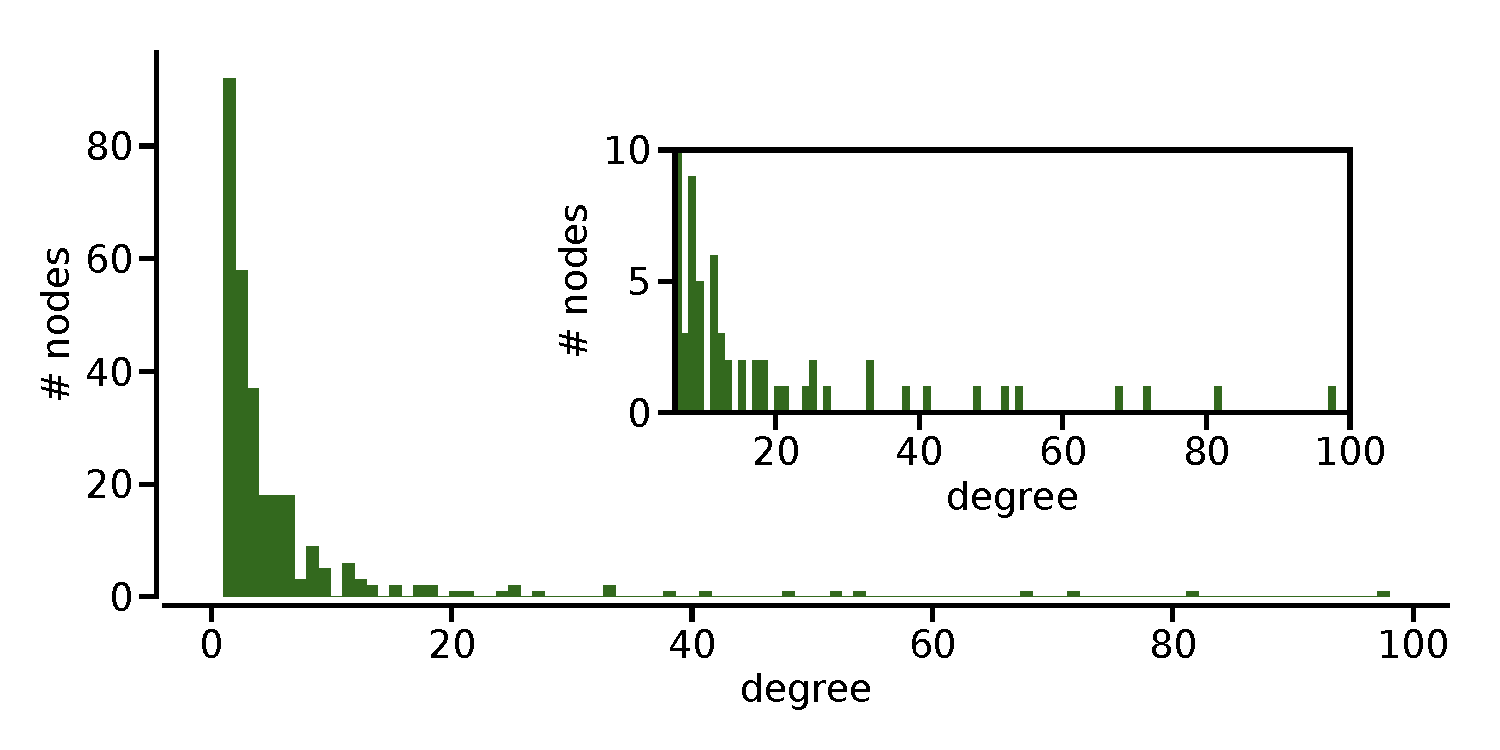
\includegraphics[width=1.0\textwidth]{figures/in-degree_distribution} \\
    (b) In-Degree Distribution
    \end{minipage}
  \end{minipage}
  \caption[In-Degree Distribution of the Citation Network]{\textbf{In-Degree Distribution.} The in-degree distribution describes how often articles get referred by other articles. The long tail of the distribution indicates that there are a lot of articles which are cited only a few times, and a few articles which are cited more often. There are some outliers with a higher degree than $20$. This can also be seen by the difference between the mean and the median. The maximum number of references in connection with the zoomed view represents that one single article was cited by $98$ other articles.}
  \label{fig:indegree_distribution}
\end{figure}

\Cref{fig:indegree_distribution} describes the in-degree distribution of our citation network. In general, the in-degree of a node is the number of ingoing edges. The in-degree distribution represents the probability distribution of these nodes over the whole network. Regarding a citation network the in-degree of a node is the number of articles which referred to this article. The long tail of the in-degree distribution indicates that there are a lot of articles which are referred only a few times, and a few articles which are referred more often. There are only some articles with an in-degree higher than $20$. The maximum number of references in connection with the zoomed view represents that one single article was referred by $98$ other articles.

\begin{figure}[!t]
  \begin{minipage}[!t]{\textwidth}
    \begin{minipage}[b]{0.39\textwidth}
      \centering
      \begin{tabular}{ l c }
        \toprule
        \textbf{Max References}    & $13$     \\ \midrule
        \textbf{Mean References}   & $2.4034$ \\ \midrule
        \textbf{Median References} & $2$      \\
        \bottomrule
    \end{tabular} \\
    \vspace*{1cm}
    (a) Properties
  \end{minipage}
  \begin{minipage}[b]{0.59\textwidth}
    \centering
    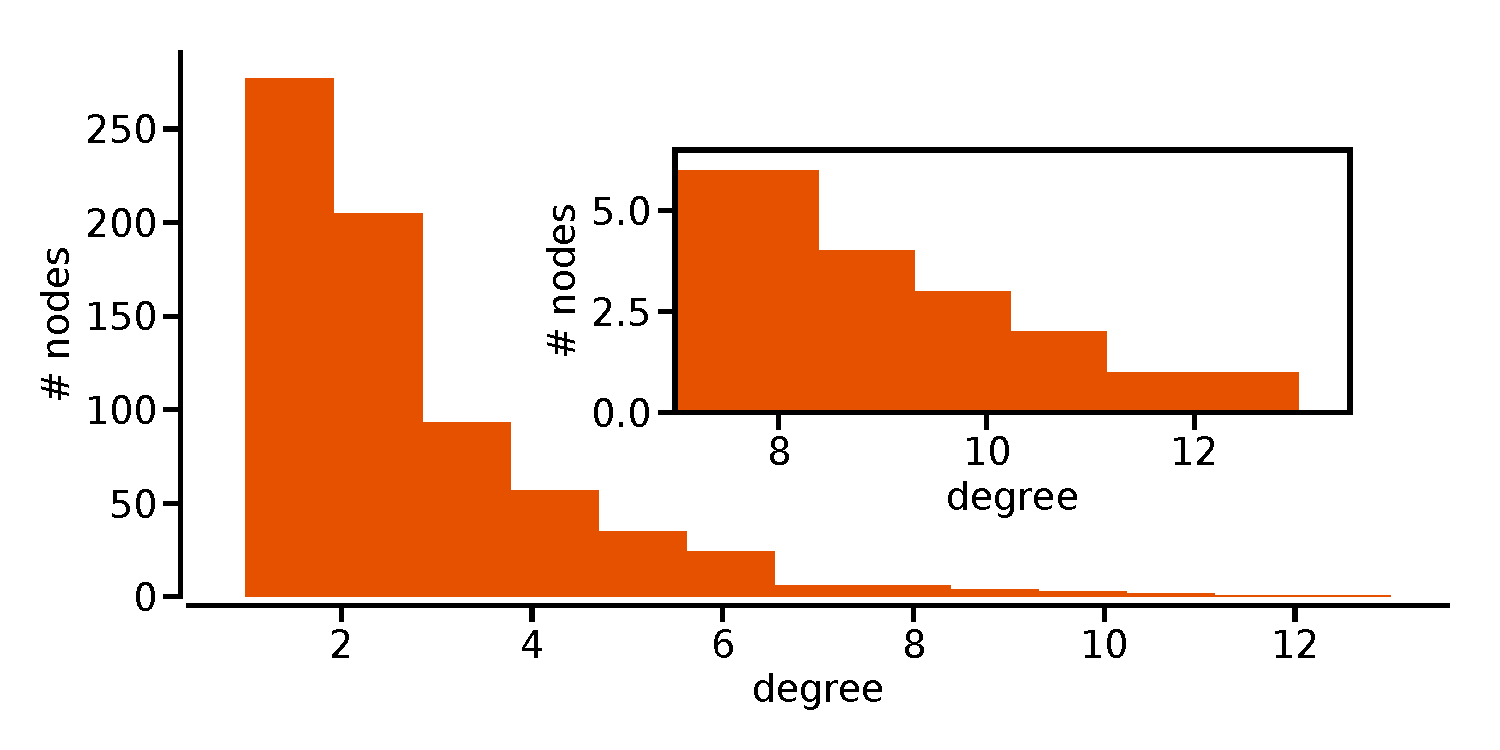
\includegraphics[width=1.0\textwidth]{figures/out-degree_distribution} \\
    (b) Out-Degree Distribution
    \end{minipage}
  \end{minipage}
\caption[Out-Degree Distribution of the Citation Network]{\textbf{Out-Degree Distribution.} The out-degree distribution describes how often articles refer other articles. The long tail of the distribution indicates that there are a lot of articles which refer less than $7$ other articles, and only few with refer to more articles. Mean and median of the outgoing edges are low, because not every refereed article is part of our dataset. By the small difference between the mean and the median can be seen that there are less outliers. The maximum number of references represent that the highest number of a single article refers other articles is $13$.}
\label{fig:outdegree_distribution}
\end{figure}

The out-degree distribution and their properties are displayed in \Cref{fig:outdegree_distribution}. In contrast to the in-degree distribution, the out-degree distribution describes the number of outgoing edges. Regarding to the citation network, the out-degree of a node can be described as the number of articles which gets referred by this article. The long tail of the out-degree distribution indicates that there are a lot of articles which refer less than $7$ other articles, and only few with refer $7$ or more articles. Mean and median of the outgoing edges are low, because not every refereed article is part of our dataset. By the small difference between mean and median we can also see that there are less outliers. The maximum number of references represent the highest number of a single article refers to other articles, which is in our case $13$.

\section{Model}
\label{sec:model}

An information retrieval model is defined by the quadruple $[\textbf{D}, \textbf{Q}, \mathcal{F}, \mathcal{R}(q_i, d_j)]$ that contains the design of documents in the document collection, queries, the framework, and the ranking function (cf. \Cref{sec:information_retrieval_models}). We design our system to compare various common ranking algorithms. Therefore we generated a model where ranking algorithm can easily be changed by a config parameter. Additionally, our model was designed to work with unstructured as well as structured data. This is reflected by the query language. 

For structured text retrieval, we structure the documents according to their IMRaD sections (see \Cref{sec:imrad_structure}). In our dataset the background chapter is available in addition to the IMRaD chapters. Therefore, it was introduced as an additional IMRaD type.

The challenge of the document definition was to provide data unstructured and structured. Hence, each document in the dataset contains a bag of words where all index terms of its text content ($DBW_{\textit{All}}$) are stored. In a bag of words each term is represented as a pair of term and term frequency. Additionally, the documents contain $5$ bag of words for each IMRaD-type ($DBW_\textit{Introduction}$, $DBW_\textit{Background}$, $DBW_\textit{Methods}$, $DBW_\textit{Results}$, $DBW_\textit{Discussion}$), where: 
\begin{align}
  DBW_\textit{IMRaD} = &DBW_\textit{Introduction} \cup DBW_\textit{Background} \cup DBW_\textit{Methods} \nonumber \\
                       &\cup DBW_\textit{Results} \cup DBW_\textit{Discussion}.
\end{align}
$DBW_\textit{IMRaD}$ differs from $DBW_{\textit{All}}$, as there exist areas in the document that cannot be assigned to an IMRaD-type (e.g., Abstract).

%\lstset{language=XML}
%\begin{lstlisting}
%<document>
%  <h1>Introduction</h1>
%  <p>I love deadlines.</p>
%  <h1>Methods</h1>
%  <p>I like the whooshing sound they make as they fly 
%     by.</p>
%</document>
%\end{lstlisting}

To generate index terms stopwords are removed and words are stemmed during the indexing process of a document. Afterwards, the index terms are assigned to bag of words of a document. For example, "\textit{I love deadlines.}" is in the \textit{Introduction} and "\textit{I like the whooshing sound they make as they fly by.}" is in the \textit{Methods} of a document $A$. The underlying bag of words in the document are given by:
\begin{equation}
  \label{bag_of_words_example_A}
  \begin{split}
  DBW_{\textit{All}} &= \{"\textit{love}": 1, "\textit{deadlin}" : 1, "\textit{whoosh}" : 1, "\textit{sound}": 1, "\textit{fly}": 1\} \\ 
  DBW_{\textit{Introduction}} &= \{"\textit{love}": 1, "\textit{deadlin}": 1\} \\
  DBW_{\textit{Methods}} &= \{"\textit{whoosh}": 1, "\textit{sound}": 1, "\textit{fly}": 1\}.
  \end{split}
\end{equation}
IMRaD sections that do not occur in the document are reflected by an empty bag of words. In this example the union of $DBW_{\textit{Introduction}}$ and $DBW_{\textit{Methods}}$ is similar to $DBW_{\textit{All}}$. When we define $A$ to additionally contain "\textit{I love music.}" in the \textit{Abstract} then $DBW_{\textit{All}}$ changes, but $DBW_{\textit{Introduction}}$ and $DBW_{\textit{Methods}}$ stay the same.

We define our query in a way that the user can choose if unstructured or structured text retrieval is used. Therefore, we design an IN-statement that connects query terms and IMRaD-Types. For example, with the query "\textit{local}, \textit{network} IN \texttt{Methods}" a user can specify that the terms \textit{local} and \textit{network} should occur in the \texttt{Methods} section of a document. The left part of the IN-statement is a set of query terms. Hence, multiple occurrences of a single term in the query does not affect the outcome. The right part of the IN-statement defines which bag of words has to be searched to find the term.

When a query contains terms without any IN-statement it denotes that unstructured text retrieval has to be used. Therefore, the terms are searched in $DBW_{\textit{All}}$. As a result query terms are searched in $DBW_{\textit{All}}$ or $DBW_\textit{IMRaD}$, but never in both of them. This query structure avoids the usage of unstructured and structured text retrieval with a single request.

We introduce an AND-statement to combine multiple IN-statements. For example, "\textit{area} IN \texttt{Background}" AND "\textit{local}, \textit{network} IN \texttt{Methods}" denotes that \textit{area} should occur in \texttt{Background} section and the terms \textit{local} and \textit{network} should occur in the \texttt{Methods} section of a document. The definition of the AND-statement leverages the possibility to search multiple bags of words with a single request. When an IMRaD type appears in multiple IN-statements the sets on the left part of the statement are combined at query time. The same holds when unstructured text retrieval is used (e.g. "\textit{area}" AND "\textit{local}, \textit{network}").

Only one query term has to occur in the specified bag of words to mark a document as relevant. This increases the number of relevant documents in the resulting ranked list. For example, a query is given by "\textit{plane} IN \texttt{Introduction}" AND "\textit{fly} IN \texttt{Methods}". When document $A$ of the previous example (see \Cref{bag_of_words_example_A}) is searched with respect to the defined query it will be marked as relevant. This happens as \textit{fly} appears in $DBW_{\textit{Methods}}$. The maximum number of relevant documents in a generated ranked list can be set via a configuration parameter. Per default this setting is disabled.   


% search with papers....

% framework
% write about: additional stored values. e.g. idf...

% ranking algorithm
% unstructured, unstructured etc.
% Write how the algorithms described in \Cref{sec:unstructured_text_Retrieval} are modified for IMRaD structure features.

\chapter{Results and Discussion}
\label{cha:results_discussion}

In this chapter we discuss the results of our information retrieval model. For our evaluation, we generated a dataset with $821$ scientific articles. Each document in the dataset was stored with its logical structure (title, headings, chapters, sections, subsections, subsubsections). Additionally, sections contain information about their IMRaD-Types. Usually a section has only one IMRaD-Type, but some of them have more (e.g., Results and Discussion are assigned the IMRaD-Types Result and Discussion). Furthermore, the articles are linked according their citations. For more information about the creation of our dataset see ~\Cref{sec:dataset}.

In our experiments we compare $5$ common ranking algorithms:
\begin{enumerate}
  \item First, \textit{Term Frequency} is the simplest approach to rank generated lists. We used \textit{Raw Frequency} of the term frequency variants. There the occurrences of each query term are counted within the document. To read more about different variants of term frequency and inverse document frequency see \Cref{sec:tfidf}.
  \item Second, \textit{TF-IDF} to take inverse document frequency into account. The inverse document frequency represents the importance of a term with respect to the entire document collection. Therefore, \textit{Inverse Frequency} is applied in combination with \textit{Raw Frequency}.
  \item Third, \textit{Okapi BM$25$} is a baseline ranking algorithm. We use the params as suggested by Robertson et. al ~\cite{RobertsonWJHG94}. Therefore, we set $b=0.75$ and $K_1 = 1$ (cf. \Cref{sec:okapi_bm25}).
  \item Fourth, \textit{Divergence from Randomness} has $2$ assumptions that are formalized with equations. In our experiments we used \Cref{dvr_part1_1} and \Cref{dvr_part2_1} for our practical implementation of the assumptions. Furthermore, \Cref{dfv_avg_doclen_1} was applied for document length normalization (cf. \Cref{sec:divergence_from_randomness}). 
  \item Fifth, \textit{Ranked Boolean Retrieval} is a ranking method that combines zone scores with boolean expressions. The score is applied to the ranking if terms occur in the zone. The configuration of the algorithm depends on the experiment (cf. \Cref{sec:ranking_strategies_in_xml_retrieval}).
\end{enumerate}


\section{Evaluation of Ranking Algorithms}
\label{sec:evaluation_of_ranking_algorithms}

The effectivity of an information retrieval system (IRS) is lean on the underlying ranking function. Therefore, it is important to measure the performance of these ranking functions to make them comparable.

\myfig{precision_recall}
      {width=0.50\textwidth}
      {\textbf{Document collection split according their relevance.} During the evaluation of a ranking algorithm the document collection is split into $4$ subsets. First, the \textit{true positive} documents retrieved as relevant for the user, which are actually relevant. Second, the \textit{false positive} documents retrieved as relevant, but are not relevant for the user. Third, the \textit{true negatives} documents were correctly received as not relevant. Forth, the \textit{false negatives} documents were incorrectly received as not relevant. The \textit{true positive} set, and \textit{true negative} set should be as large as possible as it is directly related to the effectivity of the ranking algorithm.}
      {Document collection split according their relevance.}
      {fig:precision_recall}

Evaluation of a IRS is based on the set of relevant documents provided by the system. To evaluate a generated set without any ranking (unordered) $2$ information retrieval basic measures known as \textit{Precision} and \textit{Recall} are used. \textit{Precision} is a measurement of retrieved documents (see \Cref{fig:precision_recall} for sets in the document collection split according their relevance) that are relevant for the user:
\begin{align}
  \label{precision}
  \text{Precision} = & \frac{\text{\# relevant items retrieved}}{\text{\# retrieved items}} \nonumber \\
    = & P(\text{relevant} | \text{retrieved}) \nonumber \\
    = & \frac{\text{true positives}}{\text{true positives} + \text{false positives}}.
\end{align}
\textit{Recall} represents the fraction of relevant documents that are received:
\begin{align}
  \text{Recall} = & \frac{\text{\# relevant items retrieved}}{\text{\# relevant items}} \nonumber \\
    = & P(\text{retrieved} | \text{relevant}) \nonumber \\
    = & \frac{\text{true positives}}{\text{true positives} + \text{false negatives}}.
\end{align}
There is a trade-off between the two measures. Therefore, when having a \textit{Recall} of $1$ it is possible to have a low \textit{Precision}. This happens as \textit{Recall} always increasing until all relevant documents are retrieved, but new received documents can be \textit{false positives}. Hence, the \textit{Precision} decreases, and \textit{Recall} stays the same.

There exist many different metrics to evaluate generated sets with ranking (ordered). Mean Average Precision is one of the most commonly used evaluation techniques. It is defined as the average of all precision values after a new relevant document is observed:
\begin{align}
  \label{map_of_a_single_query}
  \mathit{MAP}_i = \frac{1}{|R_i|}\sum_{k = 1}^{|R_i|} P(R_i[k]),
\end{align}
where $R_i$ is the set of relevant documents with respect to query $q_i$. $R_i[k]$ represents the reference of the $k$th document in $R_i$, and $P(R_i[k])$ is the \textit{Precision} of the document (see \Cref{precision}). If $R_i[k]$ belongs to a \textit{false positive} document $P(R_i[k]) = 0$. Furthermore, the Mean Average Precision over a set of queries is defined as:
\begin{align}
  \mathit{MAP} = \frac{1}{N_q}\sum_{i = 1}^{|N_q|} \mathit{MAP}_i,
\end{align}
where $N_q$ is the total number of queries.

\myfig{map}
      {width=1.00\textwidth}
      {\textbf{Example for Mean Average Precision of a single query.} The Precision values are calculated according the retrieved set of relevant documents. Documents with a green hook are \textit{true positives} (TP), and documents with a red cross are \textit{false positives} (FP). The precision values of FP documents are ignored for these documents, as they are not counted. In the example $R_1 =$ \{TP, FP, TP, TP, FP, TP\}, and therefore $|R_1| = 6$. Inserting these values into the Mean Average Precision formula of a single query (see \Cref{map_of_a_single_query}) results in $\mathit{MAP}_1 = 1/6 \times (1 + (2/3) + (3/4) + (4/6)) = 0.513\overline{8}$.}
      {Example for Mean Average Precision of a single query}
      {fig:map}

 Mean Average Precision is widely used as it is simple, easy to implement, versatile, and stable. Therefore, we apply it to compare the generated ranked lists of our proposed ranking algorithms (for an example see \Cref{fig:map}).


\section{Leveraging IMRaD Structure Features}
\label{sec:leveraging_imrad_structure_features}

In our first experiments we compare unstructured text retrieval with structured text retrieval. For structured text retrieval, we focus on the underlying IMRaD structure. Therefore, each document of the dataset contains a set of all index terms. In addition, they contain $5$ sets for each IMRaD-type. The union of the $5$ sets differs from the set with all index terms as there exists areas that cannot be assigned to an IMRaD-type (e.g., Abstract). 

First, we evaluate explicit search where query terms have to be formulated explicitly. For example, given a query $q_1=$"\textit{network} IN \texttt{Methods}" the system leverages different sets to search for the term. For structured text retrieval the Methods-set is used as it was specified in the query. In our system IN-statements of queries are ignored for unstructured text retrieval as all terms are searched in the set with all index terms.

Second, we discuss implicit search using entire scientific articles to search for other articles. For structured text retrieval we split the input paper according to its IMRaD-structure. We generate a query that is similar to the query of the explicit variant with the extracted terms. For unstructured text retrieval the same process is used to create the query, but IN-statements are ignored here as well.


\subsection{Explicit Search using N-Grams}

To search with information provided by the user is called explicit search. For our information retrieval model this is done by formalizing user queries. These queries can be seen as a sequence of keywords.

Our generated dataset consists of scientific articles, and links between them. We extracted citations in order to get queries that are used for testing. Our assumption was that citations describe the content of referenced articles. Therefore, a referenced article gets represented by the citation.

We store each citation as a set of terms. An important addition was that the order of the terms within the set was not lost. Additionally, we assume that a typical user searches by stringing together keywords. Therefore, we removed stopwords from the set, but terms was not stemmed. For each citation set we stored information about the refereed article, and the IMRaD-Types of the section. For example, "\textit{The authors of [$1$] present a comprehensive system for the structure extraction of PDF books, which is used within a commercial e-book software.}" is in the \textit{Introduction} of scientific article $A$. Furthermore, "\textit{[$1$]}" is the reference to the refereed scientific article $B$. The resulting citation set looks as follows: $cs_{A1} =$ \{"\textit{authors}", "\textit{present}", "\textit{comprehensive}", "\textit{system}", "\textit{structure}", "\textit{extraction}", "\textit{PDF}", "\textit{books}", "\textit{commercial}", "\textit{e-book}", "\textit{software}"\}, and additionally the reference to article $B$, and the IMRaD-Type \textit{Introduction} is stored for $cs_{A1}$.

Queries are produced as $N$-Grams with the citation sets. This means the citation sets are split into subsets of size $N$. Furthermore, the order of the terms is also important for these subsets. For example, $cs_{A1}$ is split into $N$-Grams and $N = 5$. The $7$ resulting subsets are:
\begin{align*}
  NG_{cs_{A1}, 1} &= \{"\textit{authors}", "\textit{present}", "\textit{comprehensive}", "\textit{system}", "\textit{structure}"\} \nonumber \\
  NG_{cs_{A1}, 2} &= \{"\textit{present}", "\textit{comprehensive}", "\textit{system}", "\textit{structure}", "\textit{extraction}"\} \nonumber \\
  NG_{cs_{A1}, 3} &= \{"\textit{comprehensive}", "\textit{system}", "\textit{structure}", "\textit{extraction}", "\textit{PDF}"\} \nonumber \\
  NG_{cs_{A1}, 4} &= \{"\textit{system}", "\textit{structure}", "\textit{extraction}", "\textit{PDF}", "\textit{books}"\} \nonumber \\
  NG_{cs_{A1}, 5} &= \{"\textit{structure}", "\textit{extraction}", "\textit{PDF}", "\textit{books}", "\textit{commercial}",\} \nonumber \\
  NG_{cs_{A1}, 6} &= \{"\textit{extraction}", "\textit{PDF}", "\textit{books}", "\textit{commercial}", "\textit{e-book}"\} \nonumber \\
  NG_{cs_{A1}, 7} &= \{"\textit{PDF}", "\textit{books}", "\textit{commercial}", "\textit{e-book}", "\textit{software}"\} \nonumber \\
\end{align*}
In general, the number of subsets that can be generated from a citation set $cs$ is defined as:
\begin{align}
  l = len(cs) - N + 1,
\end{align}
where $len(cs)$ is the number of terms in $cs$. 

The last step is to bring the query set together with the IMRaD-type in our query structure. For example, the resulting query compiled by $NG_{cs_{A1}, 1}$ looks as follows: $q_1=$"\textit{authors}, \textit{present}, \textit{comprehensive}, \textit{system}, \textit{structure} IN \texttt{Introduction}". In our system IN-statements of queries are ignored if IMRaD chapter features are disabled.

Mean Average Precision (see \Cref{sec:evaluation_of_ranking_algorithms}) is used to evaluate our proposed ranking algorithms. Therefore, we passed the query into our information retrieval system. The Average Precision is determined with respect to the position of the refereed article in the generated ranked list.

In \Cref{tbl:ranking_result_explicit} the performance results of our ranking algorithms are proposed. We evaluated different query lengths, where the length is defined by the number of terms in the query. Our query length varying in the range between $2$ to $14$. Furthermore, we compared the algorithms with respect to the usage of IMRaD chapter features, where disabled features denote unstructured text retrieval and enabled features represent structured text retrieval. The best results with enabled features are highlighted in violet and with disabled features are highlighted in blue for every algorithm.

All $5$ algorithms obtain higher results without IMRaD chapter features. Therefore, the ranking was generated with respect to their achieved accuracy when IMRaD chapter features are disabled. The best performing algorithm is \textit{TF-IDF}. It archives a MAP of $0.2199$ with disabled features, where the query consists of $11$ terms. In addition, the MAP is $0.1642$ with enabled features, and a query length of $12$. Therefore, the comparison of the highest accuracies is $5.57$ percent better for unstructured text retrieval. 

The second best algorithm is \textit{TF}. It has an accuracy of $0.1966$ with disabled features, and a query length of $11$. Furthermore the accuracy is $0.1293$ with enabled features, and a query length of $12$. In comparison with \textit{TF-IDF} the archived accuracy is $2.33$ percent worse for disabled features, and $3.49$ percent worse for enabled features. The best performing query lengths are the same as for \textit{TF-IDF}. The highest accuracy is $6.73$ percent better for unstructured text retrieval than for structured text retrieval.

The third best algorithm is \textit{Ranked Boolean Retrieval}. Zone scores $zs$ have to be defined to configure the algorithm (cf. \Cref{sec:ranking_strategies_in_xml_retrieval}). For the experiments only zones that contain text areas are set to a value greater zero. This was done as all citations was extracted from text areas. In our model these are text areas of sections, subsections, and subsubsections. Therefore, the constant zone scores are $zs_{\text{Section}} = 0.34$, $zs_{\text{Subsection}} = 0.33$, and $zs_{\text{Subsubsection}} = 0.33$.

\begin{table}[h]
  \begin{adjustwidth}{-2cm}{}
    \begin{tabular}{ C{1cm} C{1cm} C{2.1cm} C{2.1cm} C{2.1cm} C{2.1cm} C{2.1cm} C{2.1cm} }
      \toprule
      \textbf{\# terms in query} & \textbf{\# queries} & \textbf{Using IMRaD Chapter Features} & \textbf{Term Frequency} & \textbf{TF-IDF} & \textbf{Ranked Boolean Retrieval} & \textbf{Okapi BM$25$} & \textbf{Divergence from Randomness} \\ \midrule
      \multirow{2}{*}{$2$} & \multirow{2}{*}{$8770$} & No  & $0.0882$ & $0.1128$ & $0.1035$ & $0.0442$ & \color{blue}$\mathbf{0.0498}$  \\
                                                    && Yes & $0.0696$ & $0.0897$ & $0.0638$ & $0.045$  & \color{Plum}$\mathbf{0.0379}$  \\ \midrule
      \multirow{2}{*}{$3$} & \multirow{2}{*}{$7070$} & No  & $0.1038$ & $0.1382$ & $0.1198$ & $0.064$  & $0.046$   \\
                                                    && Yes & $0.0785$ & $0.1042$ & $0.0713$ & $0.0628$ & $0.0323$  \\ \midrule
      \multirow{2}{*}{$4$} & \multirow{2}{*}{$5589$} & No  & $0.1197$ & $0.1547$ & $0.1336$ & $0.0739$ & $0.0448$  \\
                                                    && Yes & $0.0894$ & $0.1167$ & $0.0787$ & $0.0734$ & $0.031$   \\ \midrule
      \multirow{2}{*}{$5$} & \multirow{2}{*}{$4347$} & No  & $0.1317$ & $0.1689$ & $0.1479$ & $0.0794$ & $0.0416$  \\
                                                    && Yes & $0.0993$ & $0.1262$ & $0.0844$ & $0.0791$ & $0.0317$  \\ \midrule
      \multirow{2}{*}{$6$} & \multirow{2}{*}{$3336$} & No  & $0.1469$ & $0.1766$ & $0.1603$ & $0.0804$ & $0.0396$  \\
                                                    && Yes & $0.1042$ & $0.1319$ & $0.0918$ & $0.0819$ & $0.0311$  \\ \midrule
      \multirow{2}{*}{$7$} & \multirow{2}{*}{$2550$} & No  & $0.1588$ & $0.1857$ & $0.167$  & $0.0817$ & $0.0404$  \\
                                                    && Yes & $0.1085$ & $0.1375$ & $0.0961$ & $0.0842$ & $0.0312$  \\ \midrule
      \multirow{2}{*}{$8$} & \multirow{2}{*}{$1911$} & No  & $0.1712$ & $0.1957$ & $0.1718$ & $0.0818$ & $0.0449$  \\
                                                    && Yes & $0.1158$ & $0.1441$ & $0.0988$ & $0.0916$ & $0.0303$  \\ \midrule
      \multirow{2}{*}{$9$} & \multirow{2}{*}{$1402$} & No  & $0.1804$ & $0.2074$ & $0.1757$ & $0.0879$ & $0.0456$  \\
                                                    && Yes & $0.1213$ & $0.1496$ & \color{Plum}$\mathbf{0.1015}$ & $0.0969$ & $0.0301$  \\ \midrule
      \multirow{2}{*}{$10$} & \multirow{2}{*}{$1051$} & No & $0.1847$ & $0.2153$ & $0.1851$ & $0.0952$ & $0.0466$  \\
                                                    && Yes & $0.1235$ & $0.1555$ & $0.1005$ & $0.099$  & $0.0304$  \\ \midrule
      \multirow{2}{*}{$11$} & \multirow{2}{*}{$787$} & No  & \color{blue}$\mathbf{0.1966}$ & \color{blue}$\mathbf{0.2199}$ & \color{blue}$\mathbf{0.1921}$ & $0.1075$ & $0.0439$  \\
                                                    && Yes & $0.1217$ & $0.1589$ & $0.0978$ & $0.1034$ & $0.0296$  \\ \midrule
      \multirow{2}{*}{$12$} & \multirow{2}{*}{$606$} & No  & $0.1923$ & $0.2159$ & $0.1851$ & $0.1102$ & $0.0397$  \\
                                                    && Yes & \color{Plum}$\mathbf{0.1293}$ & \color{Plum}$\mathbf{0.1642}$ & $0.0974$ & $0.1043$ & $0.0296$  \\ \midrule
      \multirow{2}{*}{$13$} & \multirow{2}{*}{$470$} & No  & $0.1846$ & $0.205$ & $0.1712$ & $0.1192$ & $0.0319$   \\
                                                    && Yes & $0.1247$ & $0.1637$ & $0.0958$ & \color{Plum}$\mathbf{0.1058}$ & $0.0295$  \\ \midrule
      \multirow{2}{*}{$14$} & \multirow{2}{*}{$362$} & No  & $0.1634$ & $0.1919$ & $0.1558$ & \color{blue}$\mathbf{0.1207}$ & $0.0221$  \\
                                                    && Yes & $0.1183$ & $0.1589$ & $0.0964$ & $0.1008$ & $0.0311$  \\
      \bottomrule
    \end{tabular}
  \caption[Ranking results with explicit search]{\textbf{Ranking results of our proposed ranking algorithms using explicit search.} We compared our proposed ranking algorithms with respect to the usage of IMRaD chapter features. Without IMRaD chapter features the entire document is used to search for query terms (unstructured). When IMRaD chapter features are enabled query terms are searched only specified sections.}
  \label{tbl:ranking_result_explicit}
  \end{adjustwidth}
\end{table}
\clearpage

\textit{Ranked Boolean Retrieval} archives an accuracy of $0.1921$ with disabled features, and a query length of $11$. Therefore, in the context of unstructured text retrieval the best performing query length is the same as for \textit{TF-IDF} and \textit{TF}. Additionally, the accuracy is $0.1015$ with enabled features, and a query length of $9$. In comparison with \textit{TF-IDF} the archived accuracy is $2.78$ percent worse for disabled features, and $6.27$ percent worse for enabled features. Furthermore, when comparing with \textit{TF} the accuracy is $0.45$ percent worse for disabled features, and $2.78$ percent worse for enabled features. The highest accuracy is $9.06$ percent better for unstructured text retrieval than for structured text retrieval.

The forth best algorithm is \textit{Okapi BM$25$}. It has an accuracy of $0.1207$ with disabled features. The associated best performing query length is $14$, which was the upper bound of the query length. It was not possible to further increase the query length as the upper bound of the query length comes with the number of queries. Furthermore, the accuracy is $0.1058$ with enabled features, and a query length of $13$. In comparison with \textit{TF-IDF} the archived accuracy is $9.92$ percent worse for disabled features, and $5.84$ percent worse for enabled features. Furthermore, when comparing with \textit{Ranked Boolean Retrieval} the accuracy is $7.14$ percent worse for disabled features, and $0.43$ percent better for enabled features. The highest accuracy is $1.49$ percent better for unstructured text retrieval than for structured text retrieval.

The fifth best algorithm is \textit{Divergence from Randomness}. It has an accuracy of $0.0498$ with disabled features, and an accuracy of $0.0379$ with enabled features. Both configurations had a best performing query length of $2$. In comparison with \textit{TF-IDF} the archived accuracy is $17.01$ percent worse for disabled features, and $12.63$ percent worse for enabled features. Furthermore, when comparing with \textit{Okapi BM$25$} the accuracy is $7.09$ percent worse for disabled features, and $6.79$ percent worse for enabled features. The highest accuracy is $1.19$ percent better for unstructured text retrieval than for structured text retrieval.

When only a few keywords are used to search for scientific articles it is not necessary to have the overhead of IMRaD chapter features. This happens as the keywords define content that should occur anywhere in the articles. Additional constraints where terms should appear are rather obstructive as they tend to hinder the finding of relevant articles.

It was unsurprisingly that \textit{TF-IDF} has a high accuracy. We used \textit{Okapi BM$25$} only with recommended parameters. A more precised parameter search would be necessary to suite our generated dataset. In comparison with the other ranking algorithms \textit{Divergence from Randomness} always had a bad performance. This bad performance is probably related to the used dataset. The good performance of \textit{Ranked Boolean Retrieval} was surprising. This probably happens as the zone scores are leveraging to hide unnecessary article areas, and mark important article areas.


\subsection{Implicit Search using Scientific Articles}
\label{sec:implicit_search_results}

In common information retrieval models there is information available that was not explicitly provided by the user. Leveraging this type of information in addition is denoted implicit search. In our model we use explicit and implicit information of scientific articles to search for other articles. This approach is called \textit{more like this}.

In our experiment we transformed scientific articles into user queries. Therefore, queries contain information about index terms and the IMRaD sections they occurred. For example, $q_1=$"\textit{structure}, \textit{present} IN \texttt{Introduction} AND \textit{system}, \textit{structure} IN \texttt{Methods}" is a query that can be executed by our system. IN-statements are used to define where the terms occurred, and AND-statements are used to combine subqueries. In our system IN-statements of queries are ignored if IMRaD chapter features are disabled.

We used a generated dataset with $821$ scientific articles to evaluate our proposed ranking algorithms. Therefore, we assumed that the content of a scientific article has to be similar to its refereed articles. As a result, the Mean Average Precision (see \Cref{sec:evaluation_of_ranking_algorithms}) is calculated with respect to the position of the refereed articles in the generated ranked list.

\begin{table}[b!]
    \centering
    \begin{tabular}{ C{2.1cm} C{2.1cm} C{2.1cm} C{2.1cm} C{2.1cm} C{2.1cm} }
      \toprule
      \textbf{Using IMRaD Chapter Features} & \textbf{Term Frequency} & \textbf{TF-IDF} & \textbf{Ranked Boolean Retrieval} & \textbf{Okapi BM$25$} & \textbf{Divergence from Randomness} \\ \midrule
      No  & $0.1186$ & $0.1163$ & $0.0466$ & $0.0554$ & $0.0137$ \\
      Yes & $0.1463$ & $0.1613$ & $0.0506$ & $0.0882$ & $0.0137$ \\
      \bottomrule
    \end{tabular}
  \caption[Ranking results using scientific articles]{\textbf{Ranking results of the used weighting schemes using scientific articles.} We compared our proposed ranking algorithms with respect to the underlying structure. Therefore, we used scientific articles unstructured and structured to search for other scientific articles. For structured articles, we focus on the underlying IMRaD structure. Mean average precision was used to evaluate the results.}
  \label{tbl:ranking_result_full}
\end{table}

In table \Cref{tbl:ranking_result_full} the performance results of our ranking algorithms are proposed. \textit{TF}, \textit{TF-IDF}, \textit{Ranked Boolean Retrieval}, and \textit{Okapi BM$25$} obtain higher results with the usage of IMRaD chapter features. \textit{Divergence from Randomness} performs with features as well as without features.

The ranking of the proposed ranking algorithms was generated with respect to their achieved accuracy when IMRaD chapter features are enabled.  The best performing algorithm is \textit{TF-IDF} with an accuracy of $0.1613$ with enabled features, and $0.1163$ with disabled features. The highest accuracy is $4.5$ percent better for structured text retrieval than for unstructured text retrieval.

The second best performing algorithm is \textit{TF}. It obtained an accuracy of $0.1463$ with enabled features, and $0.1186$ with disabled features. In comparison with \textit{TF-IDF} the archived accuracy is $1.5$ percent worse for enabled features, and $0.2$ percent better for disabled features. The highest accuracy is $2.77$ percent better for structured text retrieval than for unstructured text retrieval.

The third best performing algorithm is \textit{Okapi BM$25$}. It has an accuracy of $0.0882$ with enabled features, and $0.0554$ with disabled features. In comparison with \textit{TF-IDF} the archived accuracy is $7.31$ percent worse for enabled features, and $6.09$ percent worse for disabled features. Furthermore, when comparing with \textit{TF} the accuracy is $5.81$ percent worse for enabled features, and $6.32$ percent worse for disabled features. The highest accuracy is $3.28$ percent better for structured text retrieval than for unstructured text retrieval.

The forth best performing algorithm is \textit{Ranked Boolean Retrieval}. Zone scores $zs$ have to be defined to configure the algorithm. For the experiments the zones scores are determined through a param search, and defined as follows:
\begin{align*}
  zs_{\text{Title}} & = 0.2                \nonumber \\
  zs_{\text{Section Title}} & = 0.3        \nonumber \\
  zs_{\text{Section Text}} & = 0.2         \nonumber \\
  zs_{\text{Subsection Title}} & = 0.18    \nonumber \\
  zs_{\text{Subsection Text}} & = 0.05     \nonumber \\
  zs_{\text{Subsubsection Title}} & =0.05  \nonumber \\
  zs_{\text{Subsubsection Text}} & = 0.02, \nonumber
\end{align*}
where "Title" defines the header of the document component, and "Text" the text area of the of the document component. Fur further information about structured text retrieval, document components, and \textit{Ranked Boolean Retrieval} see \Cref{sec:structured_text_Retrieval}. 

\textit{Ranked Boolean Retrieval} has an accuracy of $0.0506$ with enabled features, and $0.0466$ with disabled features. In comparison with \textit{TF-IDF} the archived accuracy is $11.07$ percent worse for enabled features, and $6.97$ percent worse for disabled features. Furthermore, when comparing with \textit{Okapi BM$25$} the accuracy is $3.76$ percent worse for enabled features, and $0.88$ percent worse for disabled features. The highest accuracy is $0.4$ percent better for structured text retrieval than for unstructured text retrieval.

The fifth best performing algorithm is \textit{Divergence from Randomness}. It has an accuracy of $0.0137$ with enabled and disabled features. In comparison with \textit{TF-IDF} the archived accuracy is $14.76$ percent worse for enabled features, and $10.26$ percent worse for disabled features. Furthermore, when comparing with \textit{Ranked Boolean Retrieval} the accuracy is $3.69$ percent worse for enabled features, and $3.29$ percent worse for disabled features. 

When articles are used to search for other articles they can be seen as large and precised queries. IMRaD chapter features are leveraging to define these queries. This happens as constraints where terms should appear are helpful to describe the expected content of articles.

It was unsurprisingly that \textit{TF-IDF} has a high accuracy. We used \textit{Okapi BM$25$} only with recommended parameters. A more precised parameter search would be necessary to suite our generated dataset. In comparison with the other ranking algorithms \textit{Divergence from Randomness} always had a bad performance. This bad performance is probably related to the used dataset. In this experiments it can be seen that the zone scores of \textit{Ranked Boolean Retrieval} are not enough to fit the complexity of large queries. 


\section{Chapter Based Search}

\begin{table}[b!]
\vrule\pgfplotstabletypeset[%
     color cells={min=0,max=0.15,textcolor=black},
     /pgfplots/colormap={blackwhite}{rgb255=(255,170,0) color=(white) rgb255=(255,170,0)},
    /pgf/number format/fixed,
    /pgf/number format/precision=4,
    col sep=comma,
    columns/Section/.style={reset styles,string type}%
]{
Section, Introduction, Background, Methods, Results, Discussion
Introduction, 0.1242, 0.1226, 0.1095, 0.1092, 0.1049
Background,   0.1454, 0.1249, 0.1331, 0.1255, 0.1106 
Methods,      0.0947, 0.0857, 0.1017, 0.0897, 0.0668
Results,      0.0877, 0.0783, 0.0815, 0.0783, 0.0631
Discussion,   0.1188, 0.1078, 0.0957, 0.0914, 0.084
}\vrule
  \caption[Chapter based Search using TF-IDF]{\textbf{Chapter based Search using TF-IDF.} Keywords of a single chapter are used to search in single chapters of other articles. This input chapters are represented as rows, and the search chapters are represented as columns. Mean average precision was used to evaluate the results of the TF-IDF ranking algorithm.}
  \label{tbl:chapter_based_tfidf}
\end{table}

When searching with entire scientific articles we obtain better results with the usage of IMRaD chapter features in our previous experiments. Therefore, we focus on structured text retrieval and the influence of single chapters on the search result. The idea is that keywords of a chapter can be used to search in in other chapters. For example, the Methods section of one paper would be referenced in the Related Work of another paper.

We used the same dataset and evaluation process as for our implicit search evaluation (see \Cref{sec:implicit_search_results}). In our used dataset the background chapter was available in addition to the IMRaD chapters. The evaluation was done for \textit{TF-IDF} and \textit{Okapi BM$25$} as they are foundational ranking algorithms.

The chapter of the article that is used to search for other articles is defined as input chapter. Furthermore, the chapter that is searched in the articles of the collection is defined as search chapter. For example, the introduction of an article is used to search in the discussion of articles in the collection. The introduction is called input chapter and the discussion is called search chapter.

In \Cref{tbl:chapter_based_tfidf} the performance results of the \textit{TF-IDF} ranking algorithm is proposed. When \textit{Introduction}, \textit{Background}, \textit{Results}, or \textit{Discussion} is the input chapter the best results are obtained when \textit{Introduction} is the search chapter. Furthermore, when \textit{Methods} is the input chapter then the best performance is given if \textit{Methods} is also the search chapter. The highest accuracy is $0.1454$, where \textit{Background} is the input chapter, and \textit{Introduction} the search chapter. When summing up accuracies \textit{Background} is the best performing input chapter, and \textit{Introduction} the best performing search chapter.

\begin{table}[b!]
\vrule\pgfplotstabletypeset[%
     color cells={min=0.0,max=0.1,textcolor=black},
     /pgfplots/colormap={blackwhite}{rgb255=(255,170,0) color=(white) rgb255=(255,170,0)},
    /pgf/number format/fixed,
    /pgf/number format/precision=4,
    col sep=comma,
    columns/Section/.style={reset styles,string type}%
]{
Section, Introduction, Background, Methods, Results, Discussion
Introduction, 0.0884, 0.0686, 0.0631, 0.061,  0.0708
Background,   0.0909, 0.0715, 0.076,  0.0618, 0.0751
Methods,      0.0565, 0.0417, 0.0593, 0.0379, 0.0403
Results,      0.0438, 0.0426, 0.0433, 0.0461, 0.0443
Discussion,   0.0799, 0.0682, 0.0587, 0.0595, 0.0616
}\vrule
  \caption[Chapter based Search using Okapi BM$25$]{\textbf{Chapter based Search using Okapi BM$25$.} Keywords of a single chapter are used to search in single chapters of other articles. This input chapters are represented as rows, and the search chapters are represented as columns. Mean average precision was used to evaluate the results of the Okapi BM$25$ ranking algorithm.}
  \label{tbl:chapter_based_okapi}
\end{table}

In \Cref{tbl:chapter_based_okapi} the performance results of the \textit{Okapi BM$25$} ranking algorithm is proposed. When \textit{Introduction}, \textit{Background}, or \textit{Discussion} is the input chapter the best results are obtained when \textit{Introduction} is the search chapter. For \textit{Methods} and \textit{Results} the best results are obtained when they are used as input chapter as well as search chapter. The highest accuracy is $0.0909$, where \textit{Background} is the input chapter, and \textit{Introduction} the search chapter. When summing up accuracies \textit{Background} is the best performing input chapter, and \textit{Introduction} the best performing search chapter.

\textit{TF-IDF} archives better results than \textit{Okapi BM$25$} when comparing the performance results. Both ranking algorithms have \textit{Background} as their best performing input chapter, and \textit{Introduction} as their best performing search chapter. When comparing their highest accuracy \textit{TF-IDF} is $5.45$ percent better than \textit{Okapi BM$25$}. This reflects also approximately the performance of the other input chapters and search chapters.

The accuracy of implicit search with enables IMRaD chapter Features is $1.59$ percent better that the highest accuracy of search with single chapters. One interesting point is that queries for single chapters are approximately a factor of $5$ smaller than queries of implicit search, but have almost the same performance. We used \textit{Okapi BM$25$} only with recommended parameters. A more precised parameter search would be necessary to suite our generated dataset.
\chapter{Conclusion}
\label{cha:conclusion}

\section{Recap}
\label{sec:recap}

\section{Future Work}
\label{sec:future_work}


\appendix                       %% closes main document, appendix follows until end; only available in book-classes
\addpart*{Appendix}             %% adding Appendix to tableofcontents

\printbibliography              %% remove, if using BibTeX instead of biblatex
% \include{further_ressources}  %% this is a suggestion: you have to create this file on demand






%%%% end{document}
\end{document}
%% vim:foldmethod=expr
%% vim:fde=getline(v\:lnum)=~'^%%%%\ .\\+'?'>1'\:'='
%%% Local Variables:
%%% mode: latex
%%% mode: auto-fill
%%% mode: flyspell
%%% eval: (ispell-change-dictionary "en_US")
%%% TeX-master: "main"
%%% End:
